\documentclass[main.tex]{subfiles}
%tikz definitions
\tikzset{
smallnode/.style={circle, draw, very thick, minimum size=2mm},
smallcircle/.style={circle, fill, scale=0.5},
roundnode/.style={circle, draw, very thick, minimum size=10mm},
squarednode/.style={rectangle, draw, very thick, minimum size=10mm},
roundSO/.style={circle, draw, fill=gray!100, very thick, minimum size=10mm},
roundUSp/.style={circle, draw, fill=black, very thick, minimum size=10mm, text=white},
squareSO/.style={rectangle, draw, fill=gray!100, very thick, minimum size=10mm},
squareUSp/.style={rectangle, draw, fill=black, very thick, minimum size=10mm, text=white},
c1/.style={circle, draw, very thick, minimum size=1mm},
c2/.style={circle, draw, fill=black!100, very thick, minimum size=1mm}
}
\tikzset{every loop/.style={}}
\tikzset{
    arrowMe/.style={
        postaction=decorate,
        decoration={
            markings,
            mark=at position .5 with {\arrow[thick]{#1}}
        }
    }
}
\tikzset{->-/.style={decoration={
  markings,
  mark=at position .5 with {\arrow{>}}},postaction={decorate}}}
\begin{document}
\textit{The work in this chapter is based on \cite{SkHBCB}.}

\section{Introduction}
We have seen that supersymmetric theories have a moduli space $\mathbf{M}$ \eqref{eqn:intromodspacea} of supersymmetric vacua parametrised by vevs for gauge invariant, scalar, chiral operators. Moreover, for theories with eight or more supercharges we can define two interesting sub-branches of  $\mathbf{M}$, namely the Coulomb branch $\mathbf{CB}$ (in which the gauge group is typically broken to an abelian subgroup $G\to U(1)^{\dim\mathbf{CB}}$) and the Higgs branch $\mathbf{HB}$ (in which the gauge group is typically completely broken $G\to\{1\}$). For concreteness let us specialise to four dimensions. Then the Coulomb branch is reached by allowing the scalars $\Phi$ in vector multiplets to acquire vevs while setting to zero hypermultiplet vevs $(Q,\widetilde{Q})$, hence the operators on $\mathbf{CB}$ satisfy $E=-r_{\mathcal{N}=2}$ and $R_{\mathcal{N}=2}=0$. On the other hand the Higgs branch is reached by the opposite; setting $\phi=0$ while allowing $(Q,\widetilde{Q})$ to be non-zero, these have $r_{\mathcal{N}=2}=0$ and $E=2R_{\mathcal{N}=2}$. As we have seen, $\mathbf{HB}$ defined in this way turns out to be a hyperK\"ahler manifold.

Now, for generic 4d $\mathcal{N}=1$ theories, there is typically no sensible definition for analogues of $\mathbf{CB}$ and $\mathbf{HB}$. This is because, with only $\mathcal{N}=1$ supersymmetry, there is only one type of chiral multiplet who's lowest components is a scalar, whereas for $\mathcal{N}=2$ there are two (vector multiplets and hypermultiplets). Put another way, $\mathcal{N}=2$ supersymmetry has a $\rank\left(\mathfrak{su}(2)_{R_{\mathcal{N}=2}}\oplus\mathfrak{u}(1)_{r_{\mathcal{N}=2}}\right)=2$ R-symmetry algebra with which to select operators; $\mathcal{N}=1$ theories have only $\rank\mathfrak{u}(1)_r=1$.

As we will show in this chapter, if we consider a class of non-generic $\mathcal{N}=1$ theories; namely those of class $\mathcal{S}_k$, it is possible to define analogues of $\mathbf{CB}$ and $\mathbf{HB}$. Because theories of class $\mathcal{S}_k$ arise as orbifolds of $\mathcal{N}=2$ theories we can exploit the orbifold structure to define them.
\section{Moduli Space of Supersymmetric Vacua}
\label{sec:modulispace}
Gauge theories with $\mathcal{N}=1$ supersymmetry can often have a moduli space of supersymmetric vacua $\mathbf{M}$ given by the space of solutions to the F-term and D-term constraints modulo gauge transformations by gauge group $G$. It is well known \cite{Luty:1995sd}, at the level of the moduli space, that setting the D-terms to zero and modding out by $G$ is equivalent to dropping the D-term constraints and modding out by complexified gauge transformations $G^{\mathbb{C}}$. Therefore the moduli space can be described by the following symplectic quotient between the \textit{master space} $\mathbf{F}$ and the complexified gauge group
\begin{equation}\label{eqn:modspace}
\mathbf{M} \simeq \mathbf{F}/G^{\mathbb{C}}\,,\quad \mathbf{F}=\left\{(v_1,v_2,\dots)\middle|F_1=F_2=\dots=0\right\}\,,
\end{equation}
here $v_i$ denotes the scalar vevs and $F_i=\partial W/\partial v_i$ are the F-term constraints, where $W$ is the superpotential. $\mathbf{F}$ is a complex algebraic variety. It can be characterised in terms of a quotient ring $R/I$ where $R=\mathbb{C}[v_1,v_2,\dots]$ is the polynomial ring in the $v_i$ and $I=\langle F_1,F_2,\dots\rangle$ is the ideal generated by the F-terms (see Appendix \ref{Chap:AppAlgGeo} for more details regarding the \textit{algebra-geometry dictionary}) .   

In generic $\mathcal{N}=1$ gauge theories, the superpotential can receive quantum corrections up to 1-loop in perturbation theory, or from non-perturbative effects encoded in $W_{\text{n.p.}}$; for example the ADS-superpotential \cite{Affleck:1983mk}. The full superpotential can then be written as
\begin{equation}
W=W_{\text{Classical}}+W_{\text{1-loop}}+W_{\text{n.p.}}\,.
\end{equation}
The definition \eqref{eqn:modspace} can also be applied to define the moduli space of the classical theory 
\begin{gather}\label{eqn:modspaceclassical}
\mathbf{M}_{\text{Classical}} \simeq \mathbf{F}_{\text{Classical}}/G^{\mathbb{C}}\,,\\ \mathbf{F}_{\text{Classical}}=\left\{(v_1,v_2,\dots)\middle|\frac{\partial W_{\text{Classical}}}{\partial v_1}=\frac{\partial W_{\text{Classical}}}{\partial v_2}=0\right\}\,.
\end{gather}
In general $\mathbf{M}\not\iso\mathbf{M}_{\text{Classical}}$.

\subsection{The Moduli Space \texorpdfstring{$\mathbf{M}$}{M} and its Branches}
In \cite{Forcella:2008bb} and \cite{Forcella:2007wk,Forcella:2008eh,Forcella:2008ng} the moduli spaces of a large class of 4d $\mathcal{N}\geq1$ have been studied. The authors of these articles considered QFTs living on a stack of $N$ D$3$-branes with transverse space $\mathcal{X}$ a Calabi-Yau three-fold. They focused their attention on the IR physics of this system, where all the abelian symmetry decouples and the gauge symmetry is completely non-Abelian. Therefore all the abelian factors are not gauged and appear only as global symmetry of the QFT taken into account. 

In general the full moduli space $\mathbf{M}$ can have several branches, such as mesonic and baryonic branches or Coulomb and Higgs branches. Moreover these branches do not necessarily appear as irreducible components of the full moduli space but in general could be non-trivially merged into each other. Nevertheless, even if in general the baryonic and the mesonic branch are mixed, it is still makes sense to define the \textit{mesonic moduli space} ${}^{\text{mes}}\mathbf{M}$ as a sub-branch of $\mathbf{M}$. 

In order to do this, following \cite{Forcella:2008bb}, let's begin considering  the case of just one D3-brane probing the Calabi-Yau three-fold $\mathcal{X}$. The corresponding IR theory is free, therefore the moduli space $\mathbf{M}$ coincides with the master space $\mathbf{F}$.
The mesonic moduli space is obtained imposing the $U(1)_{D}$ D-term constraints. It is given by the symplectic quotient
\begin{equation}
\label{eq:mes}
{}^{\textrm{mes}}\mathbf{M} := \mathbf{M} // U(1)_{D}\, .
\end{equation}
From a physical point of view the above quotient corresponds to eliminating from the spectrum all the gauge invariants operators that are charged under the set of $U(1)_{D}$ symmetries. Therefore the branches that are eliminated taking the above quotient correspond to baryonic directions. Clearly, for the case of just one D3-brane, it's not possible to talk about baryons and the above directions are interpreted as turning on VEVs for Fayet-Iliopoulos background fields.

For the $N=1$ case of a single D$3$-brane the mesonic moduli space is simply the Calabi-Yau itself ${}^{\textrm{mes}}\mathbf{M}\iso\mathcal{X}$. The $N>1$ result is then obtained as the $N^{\text{th}}$-symmetric product of the $N=1$ case \cite{Berenstein:2002ge}, i.e.
\begin{equation}\label{eqn:symprod}
{}^{\textrm{mes}}\mathbf{M}\iso\Sym^N\left(\mathcal{X}\right)\,.
\end{equation}
The approach used in \cite{Forcella:2008bb} is based on the so called \textit{geometry-algebra dictionary}. One of the main outcomes is that, at least for the $N=1$ case, the master space always has an irreducible component that turns out to be a mesonic branch. %(in the sense of \eqref{eq:mes})
Moreover, on this branch, the scalar fields arising from all $\mathcal{N}=1$ chiral multiplet can have a non-trivial VEV. 


This algebraic approach has the advantage of providing a systematic procedure to decompose the master space of a theory into irreducible components. However, from our perspective, this procedure suffers of two main limitations:
\begin{itemize}
\item The decomposition of the master space $\mathbf{F}$ into irreducible components does not necessarily provide a decomposition of the moduli space $\mathbf{M}$ into irreducible components (an irreducible decomposition of $\mathbf{F}$ does not necessarily descend to one for the quotient $\mathbf{F}/G^{\mathbb{C}}$).
\item  The decomposition of the master space does not necessarily provide a clear identification of the Higgs branch and Coulomb branch of the theory as defined in Section \ref{sec:hc}.
\end{itemize} 

\subsubsection{An Example: $\mathcal{X}=\mathbb{C}\times\mathbb{C}^2/\mathbb{Z}_2$ Theory}\label{sec:N2example}
In order to exemplify the above statements and see how the algebraic procedure works let's review the $\mathcal{X}=\mathbb{C}\times\mathbb{C}^2/\mathbb{Z}_2 $ theory. This theory has enhanced $\mathcal{N}=2$ supersymmetry. The quiver diagram for this theory can be found in Figure \ref{fig:example}.
\begin{figure}
\center{
\begin{tikzpicture}
%nodes of the quiver
\node[roundnode] (2) {$U(1)$};
\node[roundnode] (3) [right=of 2] {$U(1)$};
\draw[-,arrowMe=<<] (2) to [bend right] (3) node [above of =2,right] {$Q_1,Q_2$};
\draw[-,arrowMe=>>] (2) to [bend left] (3) node [below of =2,right] {$\widetilde{Q}_1,\widetilde{Q}_2$};

\draw (2) edge[loop left] node {$\Phi_1$} (2);
\draw (3) edge[loop right] node {$\Phi_2$} (3);

%fields of the quivers

\end{tikzpicture}
} 
\caption{\textit{Quiver for the $\mathcal{X}=\mathbb{C}^2/\mathbb{Z}_2 \times \mathbb{C}$ theory.} \label{fig:example}}
\end{figure}
The corresponding superpotential reads
\begin{equation}
W = \Phi_1(Q_1\widetilde{Q}_1-Q_2\widetilde{Q}_2)+\Phi_2(\widetilde{Q}_2Q_2-\widetilde{Q}_1Q_1)\,. 
\end{equation}
After primary decomposition the F-terms ideal can be rewritten as
\begin{equation}
I=J_1 \cap J_2\,,\quad J_1= \langle \Phi_1-\Phi_2, \ Q_1\widetilde{Q}_1-Q_2\widetilde{Q}_2 \rangle \,,\quad J_2= \langle Q_1,Q_2,\widetilde{Q}_1,\widetilde{Q}_2 \rangle \, ,
\end{equation}
one can check that $J_1,J_2$ are \textit{prime ideals}. Therefore the master space $\mathbf{F}$ reads
\begin{equation}
\mathbf{F} = \mathfrak{V}(J_1) \cup \mathfrak{V}(J_2)\,, 
\end{equation}
where $\mathfrak{V}$ is the map that associates to each prime ideal $J$ the corresponding irreducible variety $\mathfrak{V}(J)$, defined in \eqref{eqn:mapv}. $\mathfrak{V}(J_1)=\mathbb{C}   \times   \mathcal{C}$,  is a the trivial bundle between a conifold (parametrized by $\{Q_{i=1,2},\widetilde{Q}_{i=1,2}\}$) and a $\mathbb{C}$-line (defined by $\Phi_1=\Phi_2$). On the other hand $\mathfrak{V}(J_2)$ is a $\mathbb{C}^2$ space parametrized by $\{\Phi_1,\Phi_2\}$.
Let's now consider the moduli space $\mathbf{M}$. After integration over the gauge group we observe that the variety $\mathfrak{V}(J_1)$ becomes $\mathbb{C}^2/\mathbb{Z}_2 \times \mathbb{C}$, where we can take the factor $\mathbb{C}^2/\mathbb{Z}_2$ to be parametrized by the gauge invariant combinations $\{x=Q_1\widetilde{Q}_1, y=Q_1\widetilde{Q}_2, z=Q_2\widetilde{Q}_1 \}$  that satisfy the relation $x^2=yz$. On the other hand the $\mathbb{C}$-line  factor is parametrized by $v=\Phi_1=\Phi_2$. While the second variety $\mathfrak{V}(J_2)$ does not change after the projection to gauge invariant operators. Therefore ${}^{\text{mes}}\mathbf{M}$ is given by the union of two branches that intersect in a non-trivial way. Therefore, even in this simple $\mathcal{N}=2$ example, there is \textbf{not} a clear separation between the Higgs branch (where only the scalars inside the $\mathcal{N}=2$ hypermultiplets are taking a VEV) and Coulomb branch of the theory (that is parametrized by the VEV of the scalars inside the $\mathcal{N}=2$ vector multiplet).

 
Therefore in this chapater we plan to provide a definition of the Higgs branch of a particular class of $\mathcal{N}=1$ theories without refering to the algebra-geometry dictionary. We will then outline the relation between the Higgs branch and the the mesonic branch (\ref{eq:mes}), at least in the case of the abelian theories discussed in \cite{Forcella:2008bb}.

\subsection{Higgs and Coulomb Branches for Class \texorpdfstring{$\mathcal{S}_k$}{Sk}}
\label{sec:hc}
Now let us specialise our discussion to theories in Class $\mathcal{S}_k$.
The full moduli space for these theories is typically very rich. They share many similarities with $\mathcal{N}=2$ theories, in particular they possess Coulomb, Higgs and mixed phases. On the other hand our `core theories' (see Section \ref{sec:introSk}) possess the nice property that their quantum moduli space $\mathbf{M}$ \eqref{eqn:modspace} coincides with the classial moduli space $\mathbf{M}_{\text{Classical}}$ \eqref{eqn:modspaceclassical} in the sense that, althought there may be dependence on the quantum scale $\Lambda$ it is possible always to find an isomorphism $\mathbf{M}\iso\mathbf{M}_{\text{Classical}}$. This can be seen as follows: from the point of view of the $(i,n)^{\text{th}}$ gauge node, see the quivers diagrams of Figures \ref{fig:Skquivergenus0} \& \ref{fig:Skquivergenus1}, the theory is SQCD with $N_f=3N_c$. It is known that the quantum moduli space of SQCD with $N_f\geq N_c+1$ coincides with the classical one \cite{Seiberg:1994bz}. Therefore we have
\begin{equation}
\mathbf{M}\iso\mathbf{M}_{\text{Classical}}\,,
\end{equation}
this also follows for all sub-branches, hence from now on we will refer only to $\mathbf{M}$.

The Coulomb moduli spaces of these theories have been studied in \cite{Coman:2015bqq,Razamat:2018zus}. Here we will mainly focus on two truncations of the full moduli space which, in $\mathcal{N}=2$ nomenclature, we will refer to as \textit{Higgs} and \textit{Coulomb} branches. 

\subsubsection{The Higgs Branch}\label{sec:hcbc}
Let us first present the definition for the Higgs branch for theories of class $\mathcal{S}_k$. This definition is valid for theories either with a Lagrangian description or those related to theories with a Lagrangian description by dualities and can be made by restricting to scalar operators that have
\begin{equation}\label{eqn:hbdefcharges}
 E=2R_{\mathcal{N}=2}=r+\frac{2q_t}{3}\,,\quad r_{\mathcal{N}=2}=\frac{2q_t}{3}-\frac{r}{2}=0\, ,
 \end{equation}
  where $q_t$ and $r$ denote the generators of the $\mathfrak{u}(1)_t$ and $\mathcal{N}=1$ $\mathfrak{u}(1)_{r}$ R-symmetry respectively. Provided that the R-symmetry is not broken (which is true for any $\mathcal{N}=1$ SCFT) and that $\mathfrak{u}(1)_t$ is also non-broken we can always decompose the ring $\mathcal{R}$ under the $\mathfrak{u}(1)_{r}\oplus \mathfrak{u}(1)_{t}$ grading. 

For our basic core theories corresponding to spheres with two maximal and a collection of minimal punctures (obtained by $\Phi$-gluing collections of three punctured spheres) this definition coincides with turning on generic diagonal vevs for scalars in the chiral multiplets associated to the free trinion while setting to zero vevs for the scalars in the chiral multiplets coming from $\Phi$-gluing. Those choices of vevs completely breaks the $SU(N)$ gauge symmetry at each node. Hence, we refer to this sub-branch of
$\mathbf{M}$ as the \textit{Higgs branch}
\begin{equation}\label{eqn:HB}
\mathbf{HB}=\mathbf{F_H}/G^{\mathbb{C}}\,,\quad \mathbf{F_H}=\left\{Q_{(i,n)},\widetilde{Q}_{(i,n)}\,\middle|\,F_{(j,m)}=0\right\}\,.
\end{equation}
where $Q_{(i,n)},\widetilde{Q}_{(i,n)}$ are those scalar vevs of the theory which have $r_{\mathcal{N}=2}=0$. The only non-trivial F-terms in a Lagrangian theory using the building blocks we described in Section \ref{sec:quivers} associated to a Riemann surface of genus $g$ with $\ell$ punctures on this branch are therefore just $F_{(i,n)}=\partial W_{\mathcal{S}_k}/\partial{\Phi_{(i,n)}}$ where $W_{\mathcal{S}_k}$ is given in \eqref{eqn:Sksuperpotential}.
The space $\mathbf{HB}$ is a K\"ahler manifold, as we have explained in Section \ref{sec:hibseriesintro}.

The coordinate ring of $\mathbf{F_H}$ can be described as the quotient ring $F_H=R_H/I_H$ where
\begin{gather}
R_H=\mathbb{C}[Q_{(i,n)},\widetilde{Q}_{(i,n)}]\,,\\I_H=\langle F_{(1,1)},\dots,F_{(k,1)},\dots,F_{(1,3g-3+\ell)},\dots,F_{(k,3g-3+\ell)}\rangle\,.
\end{gather}
The coordinate ring $HB$ of $\mathbf{HB}$ is given by taking the $G$-invariant polynomials $HB=(R_H/I_H)^G$.

We are now in a position to define the Higgs branch Hilbert series for our class $\mathcal{S}_k$ theories. The grading on the ring $R_H$ can be paramterised by a fugacity $\tau$ for the generator $E=2q_t=\frac{3}{2}r$, from the conditions \eqref{eqn:hbdefcharges}, as well as the fugacities for $U(1)^{k-1}_{\beta}\times U(1)^{k-1}_{\gamma}$ and any other global symmetries. The Higgs branch Hilbert series is then defined to be \cite{Feng:2007ur,Benvenuti:2006qr} 
\begin{equation}\label{eqn:HS}
\HS(\tau;HB):=\Tr_{HB}\tau^Ee^{-\mathcal{J}}\,,
\end{equation}
where $\Tr_{HB}$ denotes the trace over the space of operators parametrising the Higgs branch \eqref{eqn:HB} and $e^{-\mathcal{J}}$ collectively denotes the fugacities for the remaining intrinsic $U(1)^{k-1}_{\gamma}\times  U(1)^{k-1}_{\beta}$ and any other global symmetries. See also \cite{Gray:2008yu,Hanany:2008kn} for a detailed analysis of the Hilbert series for $\mathcal{N}=1$ SQCD. 
For gauge theories \eqref{eqn:HS} takes the general form of a integral over the gauge group $G$ of the Hilbert series of the master space $\mathbf{F_H}$ which we denote by $f_H^{\flat}$ 
\begin{equation}
\HS(\tau;HB)=\oint d\mu_G(\mathbf{z})f_H^{\flat}(\tau,\mathbf{z},\dots)\,,
\end{equation}
where $d\mu_G(\mathbf{z})$ denotes the Haar measure of $G$. 

Examining Table \ref{tab:shorts}, where short representations of the $\mathcal{N}=1$ superconformal algebra are listed, it is clear that the Hilbert series \eqref{eqn:HS} counts the top components of $\overline{\mathcal{D}}_{(0,0)}$ and $\overline{\mathcal{B}}_{r,(0,0)}$ multiplets of the $\mathcal{N}=1$ superconformal algebra. These multiplets have $E=\frac{3}{2}r$ and $j_1=j_2=0$. We can therefore see that, for $k=1$, this definition does indeed coincide with the usual Higgs branch definition for $\mathcal{N}=2$ theories.

\subsubsection{The Coulomb Branch}\label{sec:CB}
We can also make a similar definition for the Coulomb branch. Namely, analogously to $\mathcal{N}=2$ theories, we may define a consistent truncation of the moduli space by restricting those operators which have 
\begin{equation} \label{eqn:cbdefcharges}
E=-r_{\mathcal{N}=2}=-\frac{2q_t}{3}+\frac{r}{2}\,,\quad R_{\mathcal{N}=2}=\frac{r}{2}+\frac{q_t}{3}=0 \, .
\end{equation} For Lagrangian theories this coincides with setting the scalars arising from the free trinions to zero while giving the scalar in the chiral multiplets coming from the $\Phi$-gluing generic diagonal vevs. On this branch the gauge symmetry is broken down to the stabiliser subgroup of $SU(N)^{k(3g-3+\ell)}$ with respect to the vevs $\Phi_{(i,n)}$ which is given by $U(1)^{(k-1+\delta_{k,1})(3g-3+\ell)}$ where $\ell$ is the number of punctures. We have that
\begin{equation}\label{eqn:CB}
\mathbf{CB}=\mathbf{F_C}/G^{\mathbb{C}}\,,\quad \mathbf{F_C}=\left\{\Phi_{(i,n)}\right\}\,,
\end{equation}
where the $\Phi_{(i,n)}$ are those scalar vevs of the theory that have $R_{\mathcal{N}=2}=0$. On this branch all of the F-terms in a Lagrangian theory are trivial because they are all proportional to either a $Q$ or $\widetilde{Q}$. Therefore $\mathbf{F_C}$ is simply associated to the freely generated ring $R_C=\mathbb{C}[\Phi_{(i,n)}]$. Consequently $CB=(R_C)^G$.
Similarly, we may also define the Hilbert series for the Coulomb branch
\begin{equation}\label{eqn:HSCB}
\HS(T;CB):=\Tr_{CB}T^Ee^{-\mathcal{J}}\,,
\end{equation}
where $\Tr_{CB}$ denotes the trace over the space of operators parametrising \eqref{eqn:CB}. In other words, the space of scalar operators of the theory satisfying \eqref{eqn:cbdefcharges} $(E=\frac{3}{2}r=-q_t)$. Because the F-terms are trivial, for Lagrangian theories the F-flat Hilbert series \eqref{eqn:HSCB} may be computed by multiplying the contribution coming from each $\Phi$-multiplet and integrating over the gauge group. One extra simplification that arises is the fact that, because $Q=\widetilde{Q}=0$, the $(i,n)^{\text{th}}$ node in the quiver is not coupled to the $(j,m\neq n)^{\text{th}}$. Therefore \eqref{eqn:HSCB} reduces to a product of factors associated to the $\Phi$-gluing of colour $c$ and positive sign $\sigma=+$
\begin{gather}
\HS(T;CB)=\prod_{\Phi^+_c}h_{\Phi^+_c}\,,\quad h_{\Phi^+_c}=\oint d\mu\,f_{\Phi^+_c}\,,\\ f_{\Phi^+_{c}}=\prod_{i=1}^k\frac{(1-T)^{\delta_{1,k}}}{\prod_{A,B=1}^N\left(1-T\frac{\gamma_i}{\beta_{i+c-2}}\frac{z_{i,A}}{z_{i-1,B}}\right)}\,,
\end{gather} 
the $z$'s denote fugacities for the product gauge group, which are integrated over using the invariant measure $d\mu$.
We notice that the factor $f_{\Phi^+_c}=\mathcal{I}^{\text{C}}_{\Phi_c^+}$ is precisely that of the Coulomb limit of the index of the $\Phi$-gluing factor \eqref{eqn:CoulombBuild}. Therefore, we can conclude, for these Lagrangian theories that $\HS(T;CB)=\mathcal{I}^{\text{C}}$ where the Coulomb branch index is defined in \eqref{eqn:CoulombInd}. The integrals $h_{\Phi_c^+}$ have been computed in \cite{Razamat:2018zus}
\begin{equation}\label{eqn:hscbhfn}
h_{\Phi^+_c}=\PE\left[\sum_{i=1}^k\frac{\gamma^N_i}{\beta^N_{i+c-2}}T^N+\sum_{A=1}^{N-1}T^{Ak}-\delta_{1,k}T\right]\,,
\end{equation}
where $\PE$ is defined in \eqref{eqn:PE}.

\section{The Superconformal Index and Unrefined Limits}
The right-handed $\mathcal{N}=1$ superconformal index computed with respect to $\widetilde{\mathcal{Q}}_{\dot-}$ is given by \cite{Kinney:2005ej,Romelsberger:2005eg}
\begin{equation}
\begin{aligned}
\label{eqn:SCI3}
\mathcal{I}\left(t,p,q,\dots\right)=&\Tr(-1)^Fp^{j_1+j_2+\frac{r}{2}-\frac{2q_t}{3}}q^{-j_1+j_2+\frac{r}{2}-\frac{2q_t}{3}}t^{q_{t}}e^{-\mathcal{J}}e^{-\beta\widetilde{\delta}_{\dot-}}\\
=&\Tr(-1)^F\sigma^{\frac{1}{2}\delta_{1+}}\rho^{\frac{1}{2}\delta_{1-}}\tau^{\frac{1}{2}\widetilde{\delta}_{2\dot+}}e^{-\mathcal{J}}e^{-\beta'\widetilde{\delta}_{\dot-}}
\end{aligned}
\end{equation}
where $\Tr$ denotes the trace over the Hilbert space on $\mathbb{S}^3$ in the radial quantisation, $(E,j_1,j_2,r)$ denote the Cartans of the maximal compact bosonic subalgebra $\mathfrak{u}(1)_E\oplus\mathfrak{su}(2)_1\oplus\mathfrak{su}(2)_2\oplus \mathfrak{u}(1)_{r}\subset\mathfrak{su}(2,2|1)$, $q_t$ denotes the generator for the `intrinsic' global $\mathfrak{u}(1)_t$ symmetry and we have defined
\begin{gather}\label{eqn:deltas} 
\delta_{1\pm}=E\pm2j_1-\frac{r}{2}-\frac{4q_t}{3}\,,\quad \widetilde{\delta}_{2\dot\pm}=E\pm2j_2+\frac{r}{2}+\frac{4q_t}{3}\,,\\
\label{eqn:newparam}
p=\tau\sigma\,,\quad q=\tau\rho\,,\quad t=\tau^2\,.
\end{gather}
The superconformal index \eqref{eqn:SCI3} receives contributions only from those states satisfying
\begin{equation}\label{eqn:BPS2}
\widetilde{\delta}_{\dot-}=\widetilde{\delta}_{1\dot-}=2\{\widetilde{\mathcal{Q}}_{\dot-},\widetilde{\mathcal{S}}^{\dot-}\}=E-2j_2-\frac{3}{2}r=0\,.
\end{equation}
Special attention should be paid to the fugactity $t$; when $k=1$ the combinations 
\begin{equation}\label{eqn:Neq2Neq1embed}
R_{\mathcal{N}=2}=\frac{r}{2}+\frac{q_t}{3}\,,\quad r_{\mathcal{N}=2}=\frac{2q_t}{3}-\frac{r}{2}\,,
\end{equation} 
and \eqref{eqn:deltas} are elements of the enhanced $\mathfrak{su}(2,2|2)$ superconformal algebra, see Table \ref{tab:supercharges}. When $k\geq2$ there is generically no $\mathcal{N}=2$ enhancement and $q_{t}$ generates a global $U(1)_{t}$ symmetry of the corresponding theory.
Finally, $e^{-\mathcal{J}}$ collectively denotes the fugacities for the remaining intrinsic $U(1)^{k-1}_{\gamma}\times  U(1)^{k-1}_{\beta}$ and any other global symmetries.
\begin{table}
\centering
\begin{tabular}{ |c||c|c|c|c|c|c|c| } 
 \hline
 $\mathcal{Q}$ & $j_1$ & $j_2$ & $R_{\mathcal{N}=2}$ & $r_{\mathcal{N}=2}$ & $r$ & $q_t$&$\delta=2\{\mathcal{Q},\mathcal{S}\}$ \\[2pt] 
  \hline\hline
 $\mathcal{Q}_{1\pm}$ & $\pm\frac{1}{2}$ & $0$ & $+\frac{1}{2}$ & $+\frac{1}{2}$ & $+\frac{1}{3}$ & $+1$ &$\delta_{1\pm}=E\pm2j_1-\frac{r}{2}-\frac{4q_t}{3}$\\[2pt] \hline
$\mathcal{Q}_{\pm}=\mathcal{Q}_{2\pm}$ & $\pm\frac{1}{2}$ & $0$ & $-\frac{1}{2}$ & $+\frac{1}{2}$ & $-1$ & $0$&$\delta_{\pm}=\delta_{2\pm}=E\pm2j_1+\frac{3r}{2}$ \\ [2pt]\hline
$\widetilde{\mathcal{Q}}_{\dot\pm}=\widetilde{\mathcal{Q}}_{1\dot\pm}$ & $0$ & $\pm\frac{1}{2}$ & $+\frac{1}{2}$ & $-\frac{1}{2}$ & $+1$ & $0$&$\widetilde{\delta}_{\dot-}=\widetilde{\delta}_{1\dot\pm}=E\pm2j_2-\frac{3}{2}r$ \\ [2pt]\hline
$\widetilde{\mathcal{Q}}_{2\dot\pm}$ & $0$ & $\pm\frac{1}{2}$ & $-\frac{1}{2}$ & $-\frac{1}{2}$ & $-\frac{1}{3}$ & $-1$&$\widetilde{\delta}_{2\dot\pm}=E\pm2j_2+\frac{r}{2}+\frac{4q_t}{3}$ \\ [2pt]\hline
\end{tabular}
\caption{\textit{Supercharges of the $\mathfrak{su}(2,2|2)$ superalgebra and its $\mathfrak{su}(2,2|1)$ subsuperalgebra. The orbifold breaks $\mathfrak{su}(2,2|2)\xrightarrow[]{}\mathfrak{su}(2,2|1)\oplus\mathfrak{u}(1)_t$ and projects out any supercharge with $q_t\neq0$. In radial quantisation $\mathcal{S}=\mathcal{Q}^{\dagger}$.}}
\label{tab:supercharges}
\end{table}
Note that if the lowest component of a chiral superfield is given by $f$ then the fermion which also contributes to the index has 
\begin{equation}
\delta_{1\pm}[\mathcal{\widetilde{Q}}_{\dot+}\overline{f}]=2-\delta_{1\pm}[f]\,,\quad \widetilde{\delta}_{2\dot+}[\mathcal{\widetilde{Q}}_{\dot+}\overline{f}]=4-\widetilde{\delta}_{2\dot+}[f]\,.
\end{equation}
This implies that, for any chiral superfield $f$, the condition that each state contributing to the index has $\delta_{1\pm},\widetilde{\delta}_{2\dot+}\geq0$ is equivalent to
\begin{equation}
0\leq\delta_{1\pm}[f]\leq2\,,\quad 0\leq\widetilde{\delta}_{2\dot+}[f]\leq4\,.
\end{equation}
We reviewed the construction of the basic Lagrangian theories in class $\mathcal{S}_k$ in Section \ref{sec:quivers}. The letters of the free trinion of Figure \ref{fig:freetrinion} that contribute to the index are listed in Table \ref{tab:lettersft}.
\begin{table}
\centering
\begin{tabular}{|c||c|c|c|c|c|c|c|c|} 
\hline
 &  $j_1$ & $j_2$ & $r$ & $q_t$& Index&$\delta_{1+}$&$\delta_{1-}$&$\widetilde{\delta}_{2\dot+}$\\ 
 \hline\hline
  $Q_i$ & $0$ & $0$ & $\frac{2}{3}$ &$\frac{1}{2}$&$\sqrt{t}\frac{\beta_{i+c-1}}{\alpha}\chi_{l,i}\overline{\chi}_{r,i}$&$0$&$0$&$2$\\[2pt]\hline
 $\overline{\psi}_{\dot+i}$ & $0$ & $+\frac{1}{2}$ & $\frac{1}{3}$ & $-\frac{1}{2}$& $-\frac{pq}{\sqrt{t}}\frac{\alpha}{\beta_{i+c-1}}\chi_{r,i}\overline{\chi}_{l,i}$&$2$&$2$&$2$\\ [2pt]
 \hline
\hline
  $\widetilde{Q}_i$ & $0$ & $0$ & $\frac{2}{3}$ &$\frac{1}{2}$ &$\sqrt{t}\frac{\alpha}{\gamma_i}\chi_{r,i-1}\overline{\chi}_{l,i}$&$0$&$0$&$2$\\[2pt] 
 \hline
 $\overline{\widetilde{\psi}}_{\dot+i}$ & $0$ & $+\frac{1}{2}$ & $\frac{1}{3}$ &$-\frac{1}{2}$ & $-\frac{pq}{\sqrt{t}}\frac{\gamma_i}{\alpha}\chi_{l,i}\overline{\chi}_{r,i-1}$&$2$&$2$&$2$\\ [2pt]
 \hline
\hline
    $\partial_{\pm\dot+}$ &  $\pm\frac{1}{2}$ & $\frac{1}{2}$ & $0$ &$0$&  $p$, $q$&$0$, $2$&$2$, $0$&$2$, $2$\\[2pt] 
 \hline
\end{tabular}
\caption{\textit{Letters satisfying the BPS condition \eqref{eqn:BPS2} for the free trinion theory associated to a sphere with one minimal puncture (with associated $U(1)$ valued fugacity $\alpha$) and two maximal punctures $s_{c}^{l,+}$ and $s_{c+1}^{r,+}$. Here $\chi_{o,i}\equiv\chi_{(1,0,\dots,0)}(\mathbf{z}_{o,i})$, $\overline{\chi}_{o,i}\equiv\chi_{(0,0,\dots,1)}(\mathbf{z}_{o,i})$ are shorthand for the characters of the fundamental and anti-fundamental representations of $SU(N)$, defined in \eqref{eqn:SUNChar}. We importantly note that $\delta_{1\pm},\widetilde{\delta}_{2\dot+}\geq0$.}}
\label{tab:lettersft}
\end{table}
The free trinion contributes to the index a factor
\begin{equation}\label{eqn:ftindex}
\mathcal{I}_{s_{c}^{l,+},s_{c+1}^{r,+}}=\prod_{i=1}^k\prod_{A,B=1}^N\Gamma_e\left(\frac{\sqrt{t}\beta_{i+c-1}}{\alpha}\frac{z_{l,i,B}}{z_{r,i,A}}\right)\Gamma_e\left(\frac{\sqrt{t}\alpha}{\gamma_i}\frac{z_{r,i-1,B}}{z_{l,i,A}}\right)\,,
\end{equation}
where $\Gamma_e(z)$ denotes the Elliptic Gamma function, defined in \eqref{eqn:EllGamma} and with \newline$\prod_{i=1}^k\gamma_i=\prod_{i=1}^k\beta_i=1$. We will also sometimes adopt the notation $\mathcal{I}_{s_{c}^{l,+},s_{c+1}^{r,+}}=\mathcal{I}\indices{_{\mathbf{z}_l\alpha}^{\mathbf{z}_r}}$, leaving implicit the colour of the punctures. The contribution from the $\Phi$-gluing of two maximal punctures of the same sign $\sigma=+$, of colour $c$ and opposite orientation is listed in Table \ref{tab:lettersphi}. Enumerating those letters gives\footnote{The factor $\delta_{k,1}$ is to account for the fact that for $k=1$ $\Phi$ sits in the adjoint of $\mathfrak{su}(N)$ $\text{adj.}\iso \mathbf{N}\otimes\overline{\mathbf{N}}-1$, while for $k>1$ $\Phi$ sits in bifundamenal representations.}
\begin{equation}\label{eqn:tubeindex}
\mathcal{I}_{\Phi^+_c}=\prod_{i=1}^k\frac{\kappa\prod_{A,B=1}^N\Gamma_e\left(\frac{pq}{t}\frac{\gamma_i}{\beta_{i+c-2}}\frac{z_{i,B}}{z_{i-1,A}}\right)}{\Gamma_e\left(\frac{pq}{t}\right)^{\delta_{k,1}}\Delta(\mathbf{z}_{i})\prod_{A\neq B}\Gamma_e\left(\frac{z_{i,A}}{z_{i,B}}\right)}\,.
\end{equation}
The factors $\kappa$ and $\Delta$ are given by
\begin{equation}
\Delta(\mathbf{z})=\prod_{A\neq B}\left(1-\frac{z_A}{z_B}\right)\,,\quad \kappa:=(p;p)^{N-1}(q;q)^{N-1}\,.
\end{equation}
Note that in the above, and throughout, products and sums over $i$ shall always be taken modulo $k$, i.e. $i+k\sim i$ unless otherwise stated.
\begin{table}
\centering
\begin{tabular}{|c||c|c|c|c|c|c|c|c|} 
\hline
 &  $j_1$ & $j_2$ & $r$ & $q_t$& Index&$\delta_{1+}$&$\delta_{1-}$&$\widetilde{\delta}_{2\dot+}$\\ 
 \hline\hline
  $\Phi_i$ & $0$ & $0$ & $\frac{2}{3}$ &$-1$& $\frac{pq}{t}\frac{\gamma_i}{\beta_{i+c-2}}\chi_i\overline{\chi}_{i-1}$&$2$&$2$&$0$\\ [2pt]
 \hline
     $\overline{\lambda}_{\dot{+}i}$ &  $0$ & $+\frac{1}{2}$ & $+\frac{1}{3}$ &$+1$ & $-t\frac{\beta_{i+c-2}}{\gamma_i}\chi_{i-1}\overline{\chi}_i$&$0$&$0$&$4$\\ [2pt]\hline\hline
   $\lambda_{\pm i}$ & $\pm\frac{1}{2}$ & $0$ & $1$ &$0$& $-p\chi^{\text{adj.}}_i$, $-q\chi^{\text{adj.}}_i$&$0$, $2$&$2$, $0$&$2$, $2$\\ [2pt]
 \hline
  $\widetilde{F}_{\dot+\dot+i}$ &$0$ & $1$ &$0$& $0$ & $pq\chi^{\text{adj.}}_i$&$2$&$2$&$4$\\ [2pt]
 \hline
    $\partial\lambda_i=0$ & $0$ & $+\frac{1}{2}$ & $1$ &$0$ & $pq\chi^{\text{adj.}}_i$&$2$&$2$&$4$\\ [2pt]
 \hline\hline
    $\partial_{\pm\dot+}$ &  $\pm\frac{1}{2}$ & $\frac{1}{2}$ & $0$ &$0$&  $p$, $q$&$0$, $2$&$2$, $0$&$2$, $2$\\[2pt] 
 \hline
\end{tabular}
\caption{\textit{Letters satisfying the BPS condition \eqref{eqn:BPS2} of the free $\mathcal{N}=1$ theory corresponding to a tube which implements the $\Phi$-gluing of two punctures of equal colour, opposite orientation and sign $\sigma=+$. For the vector multiplet piece we must take into account the equation of motion $\partial\lambda=\partial_{+\dot+}\lambda_{-}+\partial_{-\dot+}\lambda_{+}=0$. Here $\chi_i\equiv\chi_{(1,0,\dots,0)}(\mathbf{z}_i)$, $\overline{\chi}_i\equiv\chi_{(0,0,\dots,1)}(\mathbf{z}_i)$ and $\chi^{\text{adj.}}_i\equiv\chi_{(1,0,\dots,1)}(\mathbf{z}_i)$ are shorthand for the characters of the fundamental, anti-fundamental and adjoint representations of $SU(N)$, defined in \eqref{eqn:SUNChar}. We importantly note that $\delta_{1\pm},\widetilde{\delta}_{2\dot+}\geq0$.}}
\label{tab:lettersphi}
\end{table}
For instance, we denote the $\Phi$-gluing of two three punctured spheres to obtain the theory associated to a sphere with two minimal and two maximal punctures at the level of the index by
\begin{equation}\label{eqn:4puncsphereindex}
\mathcal{I}_{s_{c}^{l,+},s_{c+2}^{r,+}}=\oint\prod_{i=1}^kd\mu_i\,I_{s_{c}^{l,+},s_{c+1}^{r,+}}\mathcal{I}_{\Phi_{c+1}^+}I_{s_{c+1}^{l,+},s_{c+2}^{r,+}}\equiv \mathcal{I}\indices{_{\mathbf{u}\alpha\delta}^{\mathbf{v}}}\,,
\end{equation}
For example, setting $k=N=c+1=2$, we can expand \eqref{eqn:4puncsphereindex} in terms of $\mathcal{N}=1$ index equivalence classes $I_{[\widetilde{r},j_1]_{\pm}}$ \eqref{eqn:indequiv} \cite{Gadde:2009dj,Beem:2012yn,Evtikhiev:2017heo} as
\begin{equation}
\begin{aligned}
&\mathcal{I}\indices{_{\mathbf{u}\alpha\delta}^{\mathbf{v}}}=1+\frac{1}{t'^2}\left[1+\frac{\beta^2}{\gamma^2}+\frac{\gamma^2}{\beta^2}\right]\mathcal{I}_{[-\frac{2}{3},0]_-}+\sum_{i=1}^2t'\left[\beta_i^2\left(\frac{1}{\alpha^2}+\frac{1}{\delta^2}\right)\right.\\
&+\gamma_i^2\left(\alpha^2+\delta^2\right)+\left(\frac{\alpha}{\delta}+\frac{\delta}{\alpha}\right)\frac{\beta_i}{\gamma_i}\chi_1(u_i)\chi_1(v_{i+1})+\beta_i\gamma_i\chi_1(v_i)\chi_1(v_{i+1})\\
&+\beta_i\gamma_i\chi_1(u_i)\chi_1(u_{i+1})\left.+\left(\alpha\delta+\frac{1}{\alpha\delta}\right)\chi_1(u_i)\chi_1(v_i)\right]\mathcal{I}_{[-\frac{2}{3},0]_-}\\
&+\sum_{i=1}^2\left[\left(\frac{\alpha\delta}{\beta_i\gamma_i}+\frac{\beta_i\gamma_i}{\alpha\delta}\right)\chi_1(u_i)\chi_1(v_{i+1})\right.\\
&\left.+\chi_2(u_i)+\chi_2(v_i)+4\vphantom{\frac{\alpha\delta}{\beta_i\gamma_i}}\right]\mathcal{I}_{[0,0]_+}+\sum_{i=1}^2\left[\left(\frac{\beta_i^3}{\alpha\delta\gamma_i}+\frac{\alpha\delta\beta_i}{\gamma_i^3}\right)\chi_1(u_i)\chi_1(v_{i+1})\right.\\
&\left.+\frac{\gamma_i^2}{\beta_i^2}\left(\chi_2(u_{i+1})+\chi_2(v_i)+1\right)\right]\mathcal{I}_{[0,0]_-}+\mathcal{O}((pq)^{4/3})
\end{aligned}
\end{equation}
where $\beta=\beta_1=\beta_2^{-1}$ and $\gamma=\gamma_1=\gamma_2^{-1}$; we have defined $t':=t/(pq)^{2/3}$ so that the expansion is made using the free R-symmetry. The equivalence class $[\frac{1}{3},\frac{1}{2}]_-$, which has only a single representative $\hat{\mathcal{C}}_{(\frac{1}{2},0)}$, contains a spin $3/2$ current and contributes to the index a factor proportional to $+(pq)^{2/3}(p+q)/(1-p)(1-q)$, is absent. This implies that either the theory has no supersymmetry enhancement, or that it contains a number of $\overline{\mathcal{B}}_{\frac{7}{3}(\frac{1}{2},0)}$ multiplets (which is the single representative of the $[\frac{1}{3},\frac{1}{2}]_+$ equivalence class) \cite{Evtikhiev:2017heo}. Note that all of the equivalence classes in the above contain only a single representative. In particular one can replace $\mathcal{I}_{[-\frac{2}{3},0]_-}=\mathcal{I}_{\overline{\mathcal{B}}_{\frac{4}{3},(0,0)}}$, $\mathcal{I}_{[0,0]_+}=\mathcal{I}_{\hat{\mathcal{C}}_{(0,0)}}$ and $\mathcal{I}_{[0,0]_-}=\mathcal{I}_{\overline{\mathcal{B}}_{2,(0,0)}}$. The \textit{net degeneracy} \cite{Beem:2012yn}, defined in \eqref{eqn:netdegen}, of the $[0,0]_{\pm}$ equivalence classes counts
\begin{equation}
\begin{aligned}
\text{ND}[0,0]=&\#[0,0]_+-\#[0,0]_-=\#\overline{\mathcal{B}}_{2,(0,0)}-\#\hat{\mathcal{C}}_{(0,0)}\\
=&\#\text{marginal operators}-\#\text{conserved currents}\\
=&30-36\,.
\end{aligned}
\end{equation}
When $k=1$ the index \eqref{eqn:SCI3} admits various interesting limits involving the three fugacities $p,q,t$ (or $\rho,\sigma,\tau$) in which the index recieves contribution only from states annihilated by two or more $\mathcal{N}=2$ Poincar\'e supercharges (one of them, of course, always being $\widetilde{\mathcal{Q}}_{\dot-}$) \cite{Gadde:2011uv}. 

Because $\widetilde{\delta}_{\dot-}[\mathcal{Q}_{\alpha}]\neq 0$ and $\widetilde{\delta}_{\dot-}[\widetilde{\mathcal{Q}}_{\dot+}]\neq0$ the index of a generic $\mathcal{N}=1$ SCFT admits no non-trivial limits in which the states contributing to it are annihilated by more than one supercharge. However, when the $\mathcal{N}=1$ SCFT has flavour symmetry, we may consider taking limits also involving the flavour fugacities. For generic theories there is no guarantee that such limits are well defined. Moreover, the index in certain limits; although not leading to extra superconformal shortening, can often admit drastic simplifications. Similar ideas have also been deployed in studying `non-generic' $\mathcal{N}=1$ SCFTs in e.g. \cite{Beem:2012yn,Gaiotto:2015usa,Rastelli:2016tbz}.

\subsection{The Hall-Littlewood Limit of the Index}
We can study the limit which, for $\mathcal{N}=2$ theories, is equivalent to the so-called Hall-Littlewood limit of the index \cite{Gadde:2011uv} \footnote{This limit has also been considered for $\mathcal{N}=1$ theories in \cite{Spiridonov:2009za,Rastelli:2016tbz}. Geometrically it corresponds to collapsing the $\mathbb{S}^3$ to a point.}
\begin{equation}
\sigma\to0\,,\quad \rho\to0\,,\quad \tau\,\,\text{fixed,}
\end{equation} 
or, equivalently, $p,q\to0$ with $t$ held fixed.  From \eqref{eqn:ftindex} and \eqref{eqn:tubeindex} we see that the Hall-Littlewood limit of the indices for the Lagrangian building blocks is well defined, we can therefore write
\begin{equation}\label{eqn:HL}
\HL(\tau,\dots):=\lim_{\sigma,\rho\to0}\mathcal{I}=\Tr_{\HL}(-1)^F\tau^{2q_t}e^{-\beta\widetilde{\delta}_{\dot-}}e^{-\mathcal{J}}\,,
\end{equation}
here $\Tr_{\HL}$ denotes the restriction of $\Tr$ to the states satisfying $\delta_{1\pm}=0$, i.e. 
$2q_t=\frac{3}{2}r+3j_2=E+j_2$ and $j_1=0$. The indices for the building blocks \eqref{eqn:ftindex} and \eqref{eqn:tubeindex} become
\begin{equation}
\HL_{s_{c}^{l,+},s_{c+1}^{r,+}}=\prod_{i=1}^k\prod_{A,B=1}^N\frac{1}{\left(1-\tau\frac{\beta_{i+c-1}}{\alpha}\frac{z_{l,i,B}}{z_{r,i,A}}\right)\left(1-\tau\frac{\alpha}{\gamma_i}\frac{z_{r,i-1,B}}{z_{l,i,A}}\right)}\label{eqn:HLFT}
\end{equation}
\begin{equation}
\HL_{\Phi_c^+}=\frac{\prod_{i=1}^k\prod_{A,B=1}^N\left(1-\tau^2\frac{\beta_{i+c-2}}{\gamma_i}\frac{z_{i-1,A}}{z_{i,B}}\right)}{\left(1-\tau^2\right)^{\delta_{k,1}}}\label{eqn:HLSglue}\,.
\end{equation}
The existence of this limit is equivalent to the fact that each letter contributing to the basic building building blocks have $\delta_{1\pm}\geq0$ (see Tables \ref{tab:lettersft} and \ref{tab:lettersphi}), as is the case for all $\mathcal{N}=2$ theories. 

As pointed out in \cite{Gadde:2011uv,Hanany:2012dm}, for class $\mathcal{S}$ theories at genus $g=0$, the Hall-Littlewood limit of the index coincides with the Hilbert series of the Higgs branch. For Lagrangian theories this can be explicitly proved and can be argued to extend to theories related to Lagrangian theories by S-duality \cite{Gaiotto:2012uq}. To the best of the authour's knowledge a full proof that extends to all class $\mathcal{S}$ theories is currently lacking. In Section \ref{sec:genuszero} we will demonstrate that the same property also holds for Lagrangian theories made using $\Phi$-gluing in class $\mathcal{S}_k$ at genus $g=0$. 

\subsection{The Coulomb Limit of the Index}
The Coulomb limit of the index for $\mathcal{N}=2$ theories is given by
\begin{equation}
\tau\to0\,,\quad \rho,\sigma\,\,\,\text{fixed,}
\end{equation}
or, equivalently, $t,p,q\to0$ with $T:=pq/t=\sigma\rho$ and $V:=p/q=\sigma/\rho$ held fixed. An extensive study of this limit of the index was given in \cite{Razamat:2018zus}. For generic $\mathcal{N}=1$ theories we would have no reason to believe that this limit exists since $\widetilde{\delta}_{2\dot+}\geq0$ is no longer guaranteed. However, let us assume that it does. In this limit the index would take the form
\begin{equation}\label{eqn:CoulombInd}
\mathcal{I}^{\text{C}}(T,V,\dots)=\Tr_{\text{C}}(-1)^FT^{E+j_2}V^{j_1}e^{-\mathcal{J}}e^{-\beta'\widetilde{\delta}_{\dot-}}
\end{equation} 
Here $\Tr_{\text{C}}$ denotes the restriction of $\Tr$ to states with $\widetilde{\delta}_{2\dot+}=0$. Indeed, we can see at the level of the Lagrangian building blocks that the limit does exist and, moreover, is conjectured to exist for all theories in class $\mathcal{S}_k$ of type $A_{N-1}$ \cite{Razamat:2018zus}. The indices for the Lagrangian building blocks \eqref{eqn:ftindex} and \eqref{eqn:tubeindex} become
\begin{equation}\label{eqn:CoulombBuild}
\mathcal{I}^{\text{C}}_{s_{c}^{l,+},s_{c+1}^{r,+}}=1\,,\quad \mathcal{I}^{\text{C}}_{\Phi^+_c}=\prod_{i=1}^k\frac{\left(1-T\right)^{\delta_{k,1}}}{\prod_{A,B=1}^N\left(1-T\frac{\gamma_i}{\beta_{i+c-2}}\frac{z_{i,B}}{z_{i-1,A}}\right)}\,.
\end{equation}
For Lagrangian theories made with $\Phi$ gluing the interpretation of this limit of the index is clear. The Coulomb limit of the index is simply counting the possible gauge invariants that can be made from the bifundamental scalar fields in the chiral multiplets $\Phi$. These operators are the top components of the $\frac{1}{2}$-BPS multiplets $\overline{\mathcal{D}}^{(-1)}_{(0,0)}$ and $\overline{\mathcal{B}}^{(-\frac{2r}{3})}_{r,(0,0)}$ which simultaneously have $E=\frac{3}{2}r=-q_t$ and $j_1=j_2=0$ (see Appendix \ref{app:SCAreps}). Indeed we will demonstrate in Section \ref{sec:CB} that, for those theories, $\mathcal{I}^{\text{C}}$ can be given the interpretation of a Hilbert series constructed to count the above $\frac{1}{2}$-BPS multiplets on the Coulomb branch.

\subsection{The Schur \& Madonald Limits of the Index}
For completeness of our discussion we can also define analogues of the Schur and Macdonald limits of the index of \cite{Gadde:2011uv}. 
The analogue of the Macdonald index is obtained by taking $\sigma\to0$, which is well defined for Lagrangian theories because each letter has $\delta_{1+}\geq0$, while holding $\rho,\tau$ fixed
\begin{equation}
\mathcal{I}^M(q,t,\dots)=\Tr_M(-1)^Fq^{-j_1+j_2+\frac{r}{2}-\frac{2q_t}{3}}t^{q_{t}}e^{-\mathcal{J}}e^{-\beta\widetilde{\delta}_{\dot-}}\,,
\end{equation} 
where $\Tr_{M}$ denotes the restriction of $\Tr$ to states with $\delta_{1+}=0$.
The Schur index is defined by setting $\rho=\tau$, or $q=t$
\begin{equation}\label{eqn:schur}
\mathcal{I}^S(q,p,\dots)=\Tr(-1)^Fp^{j_1+j_2+\frac{r}{2}-\frac{2q_t}{3}}q^{-j_1+j_2+\frac{r}{2}+\frac{q_t}{3}}e^{-\mathcal{J}}e^{-\beta\widetilde{\delta}_{\dot-}}
 \,.
\end{equation} 
Note that, unlike for $\mathcal{N}=2$ theories, the Schur index \eqref{eqn:schur} is dependent on $\sigma=p/\sqrt{q}$. However, for Lagrangian theories we have $\delta_{1+}\geq0$ and therefore we can consider a further limit, which we will call the reduced Schur index
\begin{equation}\label{eqn:redschur}
\mathcal{I}^{RS}(q,\dots):=\lim_{p\to0}\mathcal{I}^S=\Tr_{M}(-1)^Fq^{E-\frac{r}{2}-\frac{q_t}{3}}e^{-\mathcal{J}}e^{-\beta\widetilde{\delta}_{\dot-}}\equiv \mathcal{I}^M|_{q=t}\,.
\end{equation} 
In particular, for the index $\mathcal{I}^{RS}$, the Lagrangian building blocks become

\begin{equation}
\mathcal{I}^{RS}_{s_{c}^{l,+},s_{c+1}^{r,+}}=\prod_{i=1}^k\prod_{A,B=1}^N\frac{1}{\left(\sqrt{q}\frac{\beta_{i+c-1}}{\alpha}\frac{z_{l,i,B}}{z_{r,i,A}};q\right)\left(\sqrt{q}\frac{\alpha}{\gamma_i}\frac{z_{r,i-1,B}}{z_{l,i,A}};q\right)}\,,
\end{equation}
\begin{equation}
\mathcal{I}_{\Phi^+_c}^{RS}=(q;q)^{k-\delta_{k,1}}\prod_{i=1}^k\prod_{A,B=1}^N\left(q\frac{\beta_{i+c-2}}{\gamma_i}\frac{z_{i-1,A}}{z_{i,B}};q\right)\left(q\frac{z_{i,A}}{z_{i,B}};q\right)\,.
\end{equation}

For the $k=N=2$ theory associated to a sphere with two minimal punctures and two maximal punctures $s_{1}^{l,+}$, $s_{3}^{r,+}$ the reduced Schur index can be expanded as
\begin{equation}
\begin{aligned}\label{eqn:IRSexpand}
&\mathcal{I}^{RS}=1+\Big[\chi_1(m^2)\left(a^2 [0,1,0;0,0,0]+\frac{1}{a^2}[0,0,0;0,1,0]\right)\\
&+[1,0,0;0,0,1]+[0,0,1;1,0,0] \Big]q\\
&+\Big[\frac{1}{a^2}\chi_1(m^2)\left([0,0,1;1,1,0]+[1,0,0;0,1,1]\right)\\
&+a^2\chi_1(m^2)\left([1,1,0;0,0,1] + [0,1,1;1,0,0]\right)+[0,1,0;0,1,0]\\
&+[1,0,1;1,0,1]+[2,0,0;0,0,2]+[0,0,2;2,0,0]\\
&+ \chi_2(m^2)\left(a^4[0,2,0;0,0,0]+\frac{1 }{a^4}[0,0,0;0,2,0]+[0,1,0;0,1,0]\right)\Big]q^2\\
&+\mathcal{O}(q^3)\,.
\end{aligned}
\end{equation} 
Note that here, we used the symmetry enhancement of this theory \eqref{eqn:4punsymenhance}, which we will discuss in more detail in Section \ref{sec:coreint}. Here $[d_1,d_2,d_3;d_1',d_2',d_3']$ denotes the character of the enhanced $SU(2N)^k=SU(4)^2$ symmetry.

For theories with $\mathcal{N}\geq2$ supersymmetry the quantity $\mathcal{I}^S$ (which, for $\mathcal{N}\geq2$ supersymmetry, equals $\mathcal{I}^{RS}$) plays a pivotal role in the chiral algebra 2d/4d correspondence \cite{Beem:2013sza}. In particular $\mathcal{I}^S$ is identified with the vacuum character of the associated chiral algebra. 

The stress tensor of the associated chiral algebra is identified with the top component of the $\mathfrak{su}(2)_{R_{\mathcal{N}=2}}$ current, namely $j^{\mu}_{11}$. This current lives in the stress tensor multiplet $\hat{\mathcal{C}}_{0(0,0)}$ which contains conserved $\mathfrak{su}(2)_{R_{\mathcal{N}=2}}$ and $\mathfrak{u}(1)_{r_{\mathcal{N}=2}}$ currents $j^{\mu}_{(IJ)}$ and $j^{\mu}$ with $I,J=1,2$ $\mathfrak{su}(2)_{R_{\mathcal{N}=2}}$ indices. This current enters the Schur index $\mathcal{I}^S$ with a factor $\mathcal{I}^S_{\hat{\mathcal{C}}_{0(0,0)}}=q^2/(1-q)$.
Under the decomposition $\mathfrak{su}(2,2|2)\to\mathfrak{su}(2,2|1)\oplus\mathfrak{u}(1)_t$ the $\mathcal{N}=2$ stress tensor multiplet decomposes as
\begin{equation}
\hat{\mathcal{C}}_{0(0,0)}\iso\, (\hat{\mathcal{C}}_{(0,0)},0)\oplus (\hat{\mathcal{C}}_{\left(\frac{1}{2},0\right)},+1)\oplus  (\hat{\mathcal{C}}_{\left(0,\frac{1}{2}\right)},-1)\oplus (\hat{\mathcal{C}}_{\left(\frac{1}{2},\frac{1}{2}\right)},0)\,.
\end{equation}
Correspondingly, the index can be written as
\begin{equation}
\begin{aligned}
\mathcal{I}_{\hat{\mathcal{C}}_{0(0,0)}}=&\frac{-pq}{(1-p)(1-q)}+\frac{t(p+q)}{(1-p)(1-q)}+\frac{t^{-1}p^2q^{2}}{(1-p)(1-q)}\\
&+\frac{-pq(p+q)}{(1-p)(1-q)}\,;\end{aligned}
\end{equation}
see Figure \ref{fig:Chat000}. 
\begin{figure}[ht!]
\centering
\begin{tikzcd}[row sep=0.2cm, column sep=0.2cm]
&&\color{red}[0,0]^{(0)}_2\arrow[dl]\arrow[dr]&&\\
%
&\begin{tabular}{c}$\color{red}[\frac{1}{2},0]^{(-1)}_{\frac{5}{2}}$,\\
$\color{green}[\frac{1}{2},0]^{(\frac{1}{3})}_{\frac{5}{2}}$\end{tabular}\arrow[dl]\arrow[dr]&&\arrow[dl]\arrow[dr]\begin{tabular}{c}$\underbracket{\color{red}[0,\frac{1}{2}]^{(1)}_{\frac{5}{2}}\color{black}}_{\dot+}$,\\$\color{blue}[0,\frac{1}{2}]^{(-\frac{1}{3})}_{\frac{5}{2}}$\end{tabular}&\\
\color{green}[1,0]^{(-\frac{2}{3})}_{3}\arrow[dr]&&\arrow[dl]\arrow[dr]\begin{tabular}{c}
$\underbracket{\color{green}[\frac{1}{2},\frac{1}{2}]^{(\frac{4}{3})}_{3}\color{black}}_{\dot+},\color{blue}[\frac{1}{2},\frac{1}{2}]^{(-\frac{4}{3})}_{3}$, \\
$\color{red}[\frac{1}{2},\frac{1}{2}]^{(0)}_{3}\color{black},\color{cyan}[\frac{1}{2},\frac{1}{2}]^{(0)}_{3}$\end{tabular}&&\arrow[dl]\underbracket{\color{blue}[0,1]^{(\frac{2}{3})}_{3}\color{black}}_{\dot{+} \dot{+}}\\
%
&\arrow[dr]\begin{tabular}{c}$\color{cyan}[1,\frac{1}{2}]^{(-1)}_{\frac{7}{2}}$,\\
$\color{green}[1,\frac{1}{2}]^{(\frac{1}{3})}_{\frac{7}{2}}$\end{tabular}&&\begin{tabular}{c}$\underbracket{\color{cyan}[\frac{1}{2},1]^{(1)}_{\frac{7}{2}}\color{black}}_{\dot+\dot+}$,\\$\color{blue}[\frac{1}{2},1]^{(-\frac{1}{3})}_{\frac{7}{2}}$\end{tabular}\arrow[dl]&\\
&&\color{cyan}[1,1]^{(0)}_4&&
\end{tikzcd}
\caption{\textit{Branching of $\hat{\mathcal{C}}_{0(0,0)}\iso \color{red}\hat{\mathcal{C}}_{(0,0)}\color{black}\oplus \color{green}\hat{\mathcal{C}}_{\left(\frac{1}{2},0\right)}\color{black}\oplus  \color{blue}\hat{\mathcal{C}}_{\left(0,\frac{1}{2}\right)}\color{black}\oplus \color{cyan}\hat{\mathcal{C}}_{\left(\frac{1}{2},\frac{1}{2}\right)}$. Underlined are those states, with given $j_2$, which have $\widetilde{\delta}_{\dot-}=E-2j_2-\frac{3}{2}r=0$ and thus can contribute to the right-handed index \eqref{eqn:SCI3}.}}
\label{fig:Chat000}
\end{figure}
Since, the stress tensor multiplet of the mother SCFT sits in trivial representations of any flavour symmetries (e.g. it sits in a trivial $SU(N_f)$ representation) under the $\mathbb{Z}_k$ orbifold the projection of the stress tensor should simply be $\hat{\mathcal{C}}_{0(0,0)}\xrightarrow{\mathbb{Z}_k}\hat{\mathcal{C}}_{(0,0)}\oplus\hat{\mathcal{C}}_{\left(\frac{1}{2},\frac{1}{2}\right)}$. Indeed the multiplets $\hat{\mathcal{C}}_{\left(\frac{1}{2},0\right)}$ and $\hat{\mathcal{C}}_{\left(0,\frac{1}{2}\right)}$ contain additional supersymmetry currents which would lead to enhanced $\mathcal{N}\geq2$ supersymmetry if present. 

We can identify in the decomposition the $\hat{\mathcal{C}}_{(0,0)}$ as the $\mathfrak{u}(1)_t$ flavour current multiplet while $\hat{\mathcal{C}}_{\left(\frac{1}{2},\frac{1}{2}\right)}$ is of course the $\mathcal{N}=1$ stress tensor multiplet whose lowest component is the $\mathfrak{u}(1)_r$ current. They are built from linear combinations of $j^{\mu}_{12}=j^{\mu}_{21}$ and $j^{\mu}$ in accordance with \eqref{eqn:Neq2Neq1embed}. .

The currents $j^{\mu}_{11}$ and $j^{\mu}_{22}$ belong to $\hat{\mathcal{C}}_{\left(\frac{1}{2},0\right)}$ and $\hat{\mathcal{C}}_{\left(0,\frac{1}{2}\right)}$, respectively and are expected to be projected out by the orbifold. In particular we note that a factor $q^2/(1-q)$ in a trivial flavour symmetry representation does not appear in the expansion \eqref{eqn:IRSexpand}.

\section{Genus Zero Theories}\label{sec:genuszero}
In this section we consider class $\mathcal{S}_k$ theories at genus $g=0$. We show that, for this subclass of theories, the Hall-Littlewood limit of the index coincides with the corresponding Higgs branch Hilberts series. Then we provide a closed form expression for the Higgs branch Hilbert series of some Lagrangian genus zero theories, namely the free trinion and the interacting SCFT associated to a sphere with two maximal and two minimal punctures.
\subsection{Hilbert Series and the Hall-Littlewood Limit of the Index}\label{sec:HLeqHS}
We are now in a position to show that the Hall-Littlewood limit of the index coincides with the Higgs branch Hilbert series at genus $g=0$ for Lagrangian theories made using $\Phi$-gluing. For the theory corresponding to a sphere with $\ell-2$ minimal punctures and two maximal punctures the relevant F-terms for the Higgs branch are 
\begin{equation}\label{eqn:genuszeroFtermsHB}
F_{(i,n)}:=\frac{\partial W_{\mathcal{S}_k}}{\partial \Phi_{(i,n)}}= \widetilde{Q}_{(i,n-1)}Q_{(i,n-1)}-Q_{(i-1,n)}\widetilde{Q}_{(i,n)}=0\,,
\end{equation}
for $n=1,\dots,-3+\ell$ and $i+k\sim i=1,\dots, k$.
For genus $g=0$ these constitute $k(-3+\ell)$ independent constraints on the $Q_{(i,n)}$ and $\widetilde{Q}_{(i,n)}$. More precisely the ideal $I_H$ comprised of the list of the $F_{(i,n)}$ forms a regular sequence in $R_H=\mathbb{C}[Q_{(i,n)},\widetilde{Q}_{(i,n)}]$, see Appendix \ref{Chap:AppAlgGeo}. This means that the variety whose coordinate ring is given by the quotient ring $R_H/I_H$ is a complete intersection and we may apply letter counting techniques to compute the Hilbert series for the master space $\mathbf{F_H}$. 

The Hilbert series of the Higgs branch of the theory associated to the a sphere with $\ell-2$ minimal punctures and two maximal punctures $s_{1}^{l,+}$, $s_{\ell-1}^{r,+}$ is precisely given by
\begin{equation}\label{eqn:HSgenericgzero}
\HS(\tau,\dots;HB)= \oint\prod_{i=1}^k\prod_{n=2}^{\ell-2} d\mu_{(i,n)}f_H^{\flat}(\tau,\dots)
\end{equation}
\begin{equation}
f_H^{\flat}=\frac{\PE\left[\sum_{n=1}^{\ell-2}\sum_{i=1}^k\sum_{A,B=1}^N\left(\tau\frac{\beta_{i+n-1}}{\alpha_n}\frac{z_{(i,n),B}}{z_{(i,n+1),A}}+\tau\frac{\alpha_n}{\gamma_i}\frac{z_{(i-1,n+1),B}}{z_{(i,n),A}}\right)\right]}{\PE\left[\sum_{n=2}^{\ell-2}\sum_{i=1}^k\sum_{A,B=1}^N\tau^2\frac{\beta_{i+n-2}}{\gamma_i}\frac{z_{(i-1,n),A}}{z_{(i,n),B}}+(3-\ell)\tau^2\delta_{k,1}\right]}
\end{equation}
and we see that $f_H^{\flat}=\prod_{n=1}^{\ell-2}\HL_{s_{n}^{l,+},s_{n+1}^{r,+}}\prod_{n=2}^{\ell-2}\HL_{\Phi_n^+}$ and therefore $\HS\equiv\HL$ for this class of genus zero theories. The contribution of the $\overline{\lambda}_{\dot+(i,n)}$ to the Hall-Littlewood index coming from $\Phi$-gluing  precisely plays the role of the F-term constraints \eqref{eqn:genuszeroFtermsHB} in the Higgs-branch Hilbert series. 

In other words, we see that for this class of theories $\Tr_{\HL}=\Tr_{HB}$. Indeed, one can see that if one further introduces the condition $j_2=0$ into those defining the Hall-Littlewood limit of the index $\widetilde{\delta}_{\dot-}=\delta_{1\pm}=0$ we have $E=2q_t=\frac{3}{2}r$, $j_1=j_2=0$ which are precisely the conditions defining the Higgs branch \eqref{eqn:HB}.
\subsection{The Free Trinion}
Let us consider the Hall-Littlewood index/Hilbert series of the $\mathfrak{g}=A_{N-1}$ theory associated to a sphere with one minimal puncture with fugacity $\alpha$ and two maximal punctures $s_1^{l,+}$ and $s_2^{r,+}$ a.k.a. the free trinion. The expression for the Higgs branch Hilbert series was given in \eqref{eqn:HLFT} and it reads
\begin{equation}\label{eqn:HLFT2}
\HS_{s_{1}^{l,+},s_{2}^{r,+}}=\prod_{i=1}^k\prod_{A,B=1}^N\frac{1}{\left(1-\tau\frac{\beta_{i}}{\alpha}\frac{u_{i,A}}{v_{i,B}}\right)\left(1-\tau\frac{\alpha}{\gamma_i}\frac{v_{i-1,B}}{u_{i,A}}\right)}
\end{equation}
note that we set $z_l=u$ and $z_r=v$ with respect to \eqref{eqn:HLFT}.
We checked for various low values of $N$ in expansion around $\tau=0$ that the identity
\begin{equation}
\begin{aligned}
&\prod_{A,B=1}^N\frac{1}{1-a\tau \frac{u_A}{v_B}}=\sum_{l\geq0}\sum_{\lambda}(a\tau)^{Nl+\sum_{A=1}^{N-1}A(\lambda_A-\lambda_{A+1})}s_{\lambda}(\mathbf{u})s_{\overline{\lambda}}(\mathbf{v})\\
&=\sum_{\{n_1,\dots,n_N\}\geq0}(a\tau)^{\sum_{A=1}^NAn_A}\chi_{(n_1,n_2\dots,n_{N-1})}(\mathbf{u})\chi_{(n_{N-1},n_{N-2},\dots,n_1)}(\mathbf{v})
\end{aligned}
\end{equation}
holds, with $\prod_{A=1}^Nu_A=\prod_{A=1}^Nv_A=1$ and where the $SU(N)$ characters are defined in \eqref{eqn:SUNChar}. In the second line we rewrote the expression in terms of Schur polynomials, the relevant definitions and identities can be found in Appendix \ref{Chap:AppIdentities}. Therefore, we can write \eqref{eqn:HLFT2} as
\begin{equation}
\begin{aligned}
\HS_{s_{1}^{l,+},s_{2}^{r,+}}=&\sum_{l^{(j)},m^{(j)}\geq0}\sum_{\lambda^{(j)},\mu^{(j)}}\prod_{i=1}^k\Bigg\{\\
&\frac{s_{\lambda^{(i)}}(\mathbf{u}_i)s_{\overline{\mu}^{(i)}}(\mathbf{u}_i)s_{\overline{\lambda}^{(i)}}(\mathbf{v}_i)s_{\mu^{(i)}}(\mathbf{v}_{i-1})}{\prod_{A=1}^{N-1}\left(\frac{\beta_i\tau}{\alpha}\right)^{A(\lambda_{A+1}^{(i)}-\lambda_A^{(i)})-Nl^{(i)}}\left(\frac{\alpha\tau}{\gamma_i}\right)^{A(\mu_{A+1}^{(i)}-\mu_A^{(i)})-Nm^{(i)}}}\Bigg\}\,.
\end{aligned}
\end{equation}
Applying \eqref{eqn:skewdef2}
\begin{equation}
\begin{aligned}&\HS_{s_{1}^{l,+},s_{2}^{r,+}}=\\
&\sum_{\lambda^{(j)},\mu^{(j)},\nu^{(j)},\eta^{(j)}}\prod_{i=1}^k\frac{c_{\lambda^{(i)}\overline{\mu}^{(i)}}^{\eta^{(i)}}c^{\nu^{(i)}}_{\mu^{(i+1)}\overline{\lambda}^{(i)}}s_{\eta^{(i)}}(\mathbf{u}_i)s_{\nu^{(i)}}(\mathbf{v}_i)\PE\left[\frac{\alpha^N}{\gamma_i^N}\tau^N+\frac{\beta_i^N}{\alpha^N}\tau^N\right]}{\prod_{A=1}^{N-1}\left(\left(\frac{\beta_i\tau}{\alpha}\right)^{A(\lambda_{A+1}^{(i)}-\lambda_A^{(i)})}\left(\frac{\alpha\tau}{\gamma_i}\right)^{A(\mu_{A+1}^{(i)}-\mu_A^{(i)})}\right)}\,.
\end{aligned}
\end{equation}
Specialising to the case $\mathfrak{g}=A_{1}$, where we explicitly know the Littlewood-Richardson coefficients $c_{\lambda\mu}^{\nu}$, we have
\begin{equation}
\begin{aligned}
\HS_{s_{1}^{l,+},s_{2}^{r,+}}=&\prod_{i=1}^k\sum_{n_i,n'_i\geq0}\sum_{d_i=|n_i-n'_i|}^{n_i+n'_i}\sum_{d'_i=|n_i-n'_{i+1}|}^{n_i+n'_{i+1}}\Bigg\{\\
&\frac{\chi_{d_i}(u_i)\chi_{d'_i}(v_i)}{\left(1-\frac{\beta_i^2}{\alpha^2}\tau^2\right)\left(1-\frac{\alpha^2}{\gamma_i^2}\tau^2\right)}\left(\frac{\beta_i\tau}{\alpha}\right)^{n_i}\left(\frac{\alpha\tau}{\gamma_i}\right)^{n'_i}\Bigg\}\,.
\end{aligned}
\end{equation}
\subsection{Core Interacting Theories}\label{sec:coreint}
Let us first consider the Hall-Littlewood index/Higgs-branch Hilbert series for the interacting SCFT associated to a sphere with two minimal punctures and two maximal punctures $s_1^{l,+},s_{3}^{r,+}$. It is given by
\begin{equation}
\begin{aligned}
&\HL_{s^{l,+}_1,s^{r,+}_{3}}=\HL\indices{_{\mathbf{u}\delta\alpha}^{\mathbf{v}}}=\prod_{i=1}^k \oint d\mu_i\,\HL_{s^{l,+}_1,s^{r,+}_{2}}\HL_{\Phi_{2}^+}\HL_{s^{l,+}_{2},s^{r,+}_{3}}\\
&=\prod_{i=1}^k\oint d\mu_i\frac{\PE\left[\sum_{A,B=1}^N\frac{\tau\beta_{i}}{\delta}\frac{u_{i,A}}{z_{i,B}}+\frac{\tau\alpha}{\gamma_i}\frac{v_{i-1,A}}{z_{i,B}}+\frac{\tau\beta_{i+1}}{\alpha}\frac{z_{i,B}}{v_{i,A}}+\frac{\tau\delta}{\gamma_i}\frac{z_{i-1,B}}{u_{i,A}}\right]}{\PE\left[-\tau^2\delta_{k,1}+\sum_{A,B=1}^N\tau^2\frac{\beta_{i}}{\gamma_i}\frac{z_{i-1,A}}{z_{i,B}}\right]}\label{eqn:4puncHL}\,.
\end{aligned}
\end{equation}
An important observation that will allow us to write down the Highest Weight Generating (HWG) function \cite{Hanany:2014dia} for the Hilbert series for this theory is the fact that there is, at the level of the Lagrangian, a symmetry enhancement 
\begin{equation}\label{eqn:4punsymenhance}
\begin{aligned}
&SU(N)^{2k}\times U(1)_{\gamma}^{k-1}\times U(1)_{\beta}^{k-1}\times U(1)_{\delta}\times U(1)_{\alpha}\\
&\to SU(2N)^{k}\times U(1)_{a}^{k-1} \times U(1)_{m}\,,
\end{aligned}
\end{equation}
which we can make manifest in \eqref{eqn:4puncHL} by writing
\begin{equation}
\mathbf{x}_i=\left(\sqrt{\frac{\gamma_i\beta_i}{\delta\alpha}}\mathbf{u}_i,\sqrt{\frac{\delta\alpha}{\gamma_i\beta_i}}\mathbf{v}_{i-1}\right)\,,\quad a_i=\sqrt{\frac{\beta_i}{\gamma_i}}\,,\quad m=\sqrt{\frac{\alpha}{\delta}}\,,
\end{equation}
corresponding to writing $q_i=(Q_i^L,\widetilde{Q}_{i-1}^R)$, $\widetilde{q}_i=(\widetilde{Q}_i^L,Q^R_{i-1})$ in the decomposition $\mathbf{2N}\to(\mathbf{N},\mathbf{1})_1\oplus(\mathbf{1},\mathbf{N})_{-1}$ under $SU(2N)\to SU(N)\times SU(N)\times U(1)$ and $Q_i^L,\widetilde{Q}_{i}^L$ are the bifundamental chiral multiplets of the first free trinion and $Q_i^R,\widetilde{Q}_{i}^R$ the second. Then the Hall-Littlewood index / Hilbert series can be written as
\begin{equation}\label{eqn:HSfull4punc}
\begin{aligned}
&\HS_{s^{l,+}_1,s^{r,+}_{3}}=\\
&\prod_{i=1}^k\oint\prod_{A=1}^{N-1}\frac{dz_{i,A}}{2\pi\iu z_{i,A}}\frac{\prod\limits_{1\leq A<B\leq N}\left(1-\frac{z_{i,B}}{z_{i,A}}\right)\prod_{A,B=1}^N\left(1-\tau^2a_i^2\frac{z_{i-1,A}}{z_{i,B}}\right)}{(1-\tau^2)^{\delta_{k,1}}\prod\limits_{A=1}^N\prod\limits_{B=1}^{2N}\left(1-\tau a_im\frac{x_{i,B}}{z_{i,A}}\right)\left(1-\tau\frac{a_i}{m}\frac{z_{i-1,A}}{x_{i,B}}\right)}\,.
\end{aligned}
\end{equation}
The symmetry enhancement \eqref{eqn:4punsymenhance} allows us to conjecture the following expression for the Highest Weight Generating (HWG) function for the Hilbert series as
\begin{equation}
\begin{aligned}
\HWG_{s^{l,+}_1,s^{r,+}_{3}}=\PE\Bigg[&\delta_{1,k}\tau^2+\sum_{i=1}^k\sum_{A=1}^{N-1}\mu^{(i)}_{A}\mu^{(i+1)}_{2N-A}a_i^Aa_{i+1}^A\tau^{2A}\\
&+\sum_{i=1}^k\mu^{(i)}_{N}a_i^{N}\left(m^{N}+\frac{1}{m^N}\right)\tau^N\Bigg]\, \ ,
\end{aligned}
\end{equation}
where $\{\mu_{A}^{(i)}\}$ denotes a set of highest weights for the $i^{\text{th}}$ flavour node.
From the HWG one then obtains the Hilbert series by replacing 
\begin{equation}
\prod_{A=1}^{2N-1}{\mu^{(i)}_A}^{d_A}\leftrightarrow[d_1,d_2,\dots,d_{2N-1}]_{\mathbf{x}_i}
\end{equation}
where $[d_1,d_2,\dots,d_{2N-1}]_{\mathbf{x}}\equiv\chi_{(d_1,d_2,\dots,d_{2N-1})}(\mathbf{x})$ denotes the character of $SU(2N)$, defined in \eqref{eqn:SUNChar}.
The Hilbert series is given by
\begin{equation}\label{eqn:HSconject}
\begin{aligned}
& \HS_{s^{l,+}_1,s^{r,+}_{3}}=\left(1-\tau^2\right)^{-\delta_{1,k}}\sum_{\{n^{(i)}_{A},p^{(i)},l^{(i)}\geq0\}}\prod_{i=1}^k\Bigg\{\\
&\left[n^{(i)}_{1},n^{(i)}_{2},\dots,n^{(i)}_{N-1},p^{(i)}+l^{(i)},n^{(i+1)}_{N-1},n^{(i+1)}_{N-2},\dots,n^{(i+1)}_{1}\right]_{\mathbf{x}_i}\\
& m^{Np^{(i)}-Nl^{(i)}}a_i^{Np^{(i)}+Nl^{(i)}+\sum_{A=1}^{N-1}An_{A}^{(i)}}a_{i+1}^{\sum_{A=1}^{N-1}An_{A}^{(i+1)}}\tau^{Np^{(i)}+Nl^{(i)}+2\sum_{A=1}^{N-1}An^{(i)}_{A}}\Bigg\}\,.
\end{aligned}
\end{equation}
We checked in an expansion around $\tau=0$ that \eqref{eqn:HSconject} agrees with \eqref{eqn:HSfull4punc} for $(N,k)=\{(2,2),(2,3),(3,2)\}$. For theories associated to $\ell$-punctured spheres with two maximal punctures and $\ell-2>2$ minimal punctures there is no symmetry enhancement \eqref{eqn:4punsymenhance} and the number of monomials in the $\PLog$ of the HWG is not finite. This means that it is not practically possible to write down a closed form expression for the HWG. 

We can however perform the expansion of the integral \eqref{eqn:HSgenericgzero} around $\tau=0$. For example, for $k=N=2$, $\ell-2=3$ we have
\begin{equation}
\begin{aligned}
&\HS=1+ \Bigg[\chi^L_{2} \chi^L_{1}\left(\frac{\beta }{\gamma }+\frac{\gamma }{\beta }\right)\\
& +\chi^R_{2}\chi^R_{1} \left(\beta  \gamma +\frac{1}{\beta  \gamma }\right)+\sum_{n=1}^{3}\sum_{i=1}^2\left(\frac{\beta^2_i}{\alpha _n^2}+\gamma_i^2\alpha _n^2\right)\Bigg]\tau^2\\
&+\left[\left(\frac{\alpha
   _3 \alpha _2}{\alpha _1}+\frac{\alpha _1 \alpha _2}{\alpha _3}+\frac{\alpha _1 \alpha _3}{\alpha _2}+\frac{1}{\alpha _1 \alpha _3 \alpha _2}\right) \sum_{i=1}^2\beta_i\chi_i^L\chi_i^R\right.\\
   &\,\,+\left.\left(\alpha _2 \alpha _3 \alpha _1+\frac{\alpha _1}{\alpha _2 \alpha _3}+\frac{\alpha _3}{\alpha _2 \alpha _1}+\frac{\alpha _2}{\alpha _3 \alpha _1}\right) \sum_{i=1}^2\gamma_{i+1}\chi^L_i\chi_{i+1}^R\right]\tau ^3 +\mathcal{O}(\tau^4)
   \end{aligned}
\end{equation}
where $\beta_1=\frac{1}{\beta_2}=\beta$, $\gamma_1=\frac{1}{\gamma_2}=\gamma$ and $\chi^L_{i}=\chi_{1}(z_{(i\bmod k,1)})$, $\chi^R_{i}=\chi_{1}(z_{(i\bmod k,4)})$ denotes the characters of the fundamental representation of the corresponding $SU(2)$'s.
\section{Genus One Theories}\label{sec:hsg1}
In this section we consider some theories that are closely related to class $\mathcal{S}_k$ theories at genus one. The theories that we study are the $\mathcal{N}=1$ $\mathfrak{u}(N)^{\oplus\ell k}$ toroidal quiver gauge theories realised as the $l_s\to0$ limit of the worldvolume theory on a stack of $N$ D3-branes probing a transverse $\mathbb{C}^3/(\mathbb{Z}_{\ell}\times\mathbb{Z}_k)$ singularity where the quotient acts by
\begin{equation}\label{eqn:quotientactZkZl}
(z_1,z_2,z_3)\mapsto(\omega_kz_1,\omega_{\ell}z_2,\omega_{\ell}^{-1}\omega^{-1}_{k}z_3)\,,\quad \omega_k^k=\omega_{\ell}^{\ell}=1\,.
\end{equation}
These are orbifolds of $\mathcal{N}=4$ SYM; we discussed them at length in Section \ref{sec:quivers}. In the case where the $\mathfrak{u}(1)^{\oplus\ell k}\subset\mathfrak{u}(N)^{\oplus\ell k}$ is not gauged, these are precisely the theories in class $\mathcal{S}_k$ associated to Riemann surfaces of genus one with $\ell$ punctures. 

The action \eqref{eqn:quotientactZkZl} is an element of the $SO(6)_R$ R-symmetry group of $\mathcal{N}=4$ SYM. If we denote the $\mathcal{N}=4$ supercharges by $\mathcal{Q}_{\alpha}^{q_1q_2q_3}$ with $8q_1q_2q_3=-1$ and $\overline{\mathcal{Q}}_{\dot\alpha}^{q_1q_2q_3}$ with $8q_1q_2q_3=+1$ where the $q_i=\pm\frac{1}{2}$. The orbifold acts by
\begin{equation}
\mathcal{Q}_{\alpha}^{q_1q_2q_3}\mapsto \omega_k^{q_1-q_3}\omega_{\ell}^{q_2-q_3}\mathcal{Q}_{\alpha}^{q_1q_2q_3}\,,\quad
\overline{\mathcal{Q}}_{\dot\alpha}^{q_1q_2q_3}\mapsto \omega_k^{q_1-q_3}\omega_{\ell}^{q_2-q_3}\overline{\mathcal{Q}}_{\dot\alpha}^{q_1q_2q_3}\,.
\end{equation}
The surviving supercharges are those with $q_1=q_2=q_3$
\begin{equation}
\mathcal{Q}_{\alpha}^{---}=\mathcal{Q}_{\alpha}\,,\quad\overline{\mathcal{Q}}^{+++}_{\dot\alpha}=\overline{\mathcal{Q}}_{\dot\alpha}\,.
\end{equation}
The Cartans $q_1,q_2,q_3$ of $\mathfrak{so}(6)_R$ are related to the more natural $\mathcal{N}=1$ symmetries by
\begin{equation}\label{eqn:N4N1ides}
r=\frac{2}{3}(q_1+q_2+q_3)\,,\quad q_t=-q_1+\frac{1}{2}(q_2+q_3)\,,\quad q_b=-q_2+q_3\,,
\end{equation} 
there is also the overall $U(1)$ generated by $b$.

It will later be useful to have to hand the Hilbert series for this quotient space. This is given by the \textit{Molien series}
\begin{equation}
\begin{aligned}\label{eqn:moilen}
M(\tau_1,\tau_2,\tau_3;\mathbb{C}^3/(\mathbb{Z}_{\ell}\times\mathbb{Z}_k))&=\frac{1}{\ell k}\sum_{\substack{g\in\mathbb{Z}_{\ell}\\h\in\mathbb{Z}_k}}\PE\left[h\tau_1+g\tau_2+g^{-1}h^{-1}\tau_3\right]\\
&=\frac{\sum_{r=0}^{LCM(\ell,k)-1}(\tau_1\tau_2\tau_3)^r\tau_1^{-\lfloor\frac{r}{k}\rfloor k}\tau_2^{-\lfloor\frac{r}{\ell}\rfloor\ell}}{(1-\tau_1^k)(1-\tau_2^{\ell})(1-\tau_3^{LCM(\ell,k)})}
\,,\end{aligned}
\end{equation}
where $\tau_1,\tau_2,\tau_3$ are related to the $SO(6)_R\supset U(1)^{3}\lefttorightarrow\mathbb{C}^3$ toric action generated by $q_1,q_2,q_3$. Moreover $LCM(\ell,k)$ denotes the Lowest Common Multiple of $\ell$ and $k$. For $\ell=k$ these varieties are complete intersections since 
\begin{equation}
M(\tau_1,\tau_2,\tau_3;\mathbb{C}^3/(\mathbb{Z}_{k}\times\mathbb{Z}_k))=\PE\left[\sum_{n=1}^3\tau_n^k+\tau_1\tau_2\tau_3-\tau_1^k\tau_2^k\tau_3^k\right]\,.
\end{equation}
This space can be realised as $\mathbb{C}^3/(\mathbb{Z}_{k}\times\mathbb{Z}_k)\hookrightarrow\mathbb{C}^4$ defined by the equation
\begin{equation}
w_1w_2w_3-w_4^k=0\,,
\end{equation}
with $w_i=z_i^k$, $w_4=z_1z_2z_3$.
As a warm up we will now review the computation for $k=1$.
\subsection{Class \texorpdfstring{$\mathcal{S}$}{S}}
We reviewed this theory and it's moduli space $\mathbf{M}$ for $\ell=2$ in detail in Section \ref{sec:N2example}. The quiver diagram for this theory is given in Figure \ref{fig:quivercircular}.
\begin{figure}
\begin{center}
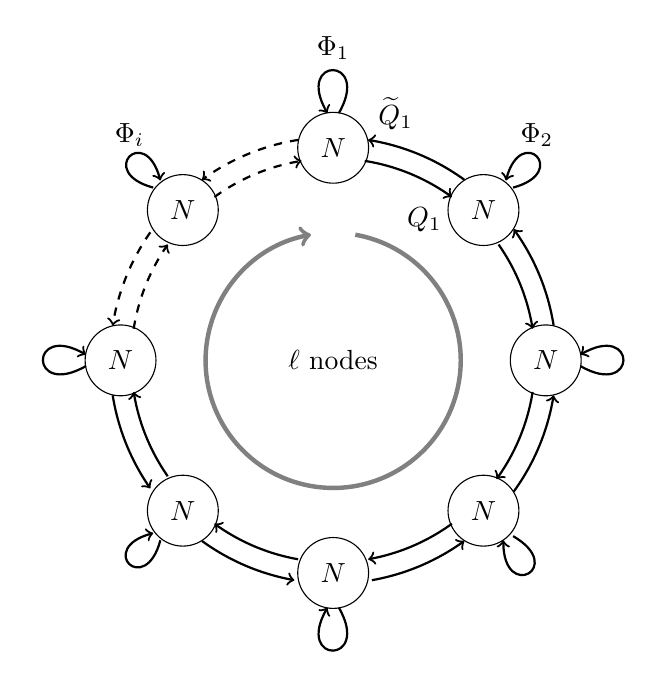
\begin{tikzpicture}[scale=0.9]
\def\circledarrow#1#2#3{ % #1 Style, #2 Center, #3 Radius
\draw[#1,->] (#2) +(80:#3) arc(80:-260:#3);
}
 
%set of the different gauge nodes

\draw (0,3) circle [radius=0.5]  node (A) {$N$};
\draw (1.5*1.414,1.5*1.414)  circle [radius=0.5] node {$N$};
\draw (3,0)  circle [radius=0.5] node {$N$};
\draw (1.5*1.414,-1.5*1.414)  circle [radius=0.5] node {$N$};
\draw (0,-3)  circle [radius=0.5] node {$N$};
\draw (-1.5*1.414,-1.5*1.414)  circle [radius=0.5] node {$N$};
\draw (-3,0)  circle [radius=0.5] node {$N$};
\draw (-1.5*1.414,1.5*1.414)  circle [radius=0.5] node {$N$};


%bifundamentals fields

\draw [->,thick,domain=54:81,scale=3] plot ({1.05*cos(\x)}, {1.05*sin(\x)}) node[above right] {$\widetilde{Q}_1$};
\draw [->,thick,domain=81:54,scale=3] plot ({0.95*cos(\x)}, {0.95*sin(\x)}) node[below left] {$Q_1$};;

\draw [->,thick,domain=9:36,scale=3] plot ({1.05*cos(\x)}, {1.05*sin(\x)});
\draw [->,thick,domain=35:9,scale=3] plot ({0.95*cos(\x)}, {0.95*sin(\x)});

\draw [<-,thick,domain=-9:-36,scale=3] plot ({1.05*cos(\x)}, {1.05*sin(\x)});
\draw [<-,thick,domain=-36:-9,scale=3] plot ({0.95*cos(\x)}, {0.95*sin(\x)});

\draw [<-,thick,domain=-54:-80,scale=3] plot ({1.05*cos(\x)}, {1.05*sin(\x)});
\draw [<-,thick,domain=-80:-54,scale=3] plot ({0.95*cos(\x)}, {0.95*sin(\x)});

\draw [->,thick,domain=54:80,scale=-3] plot ({1.05*cos(\x)}, {1.05*sin(\x)});
\draw [->,thick,domain=80:54,scale=-3] plot ({0.95*cos(\x)}, {0.95*sin(\x)});

\draw [->,thick,domain=9:35,scale=-3] plot ({1.05*cos(\x)}, {1.05*sin(\x)});
\draw [->,thick,domain=35:9,scale=-3] plot ({0.95*cos(\x)}, {0.95*sin(\x)});

\draw [->,dashed,thick,domain=-35:-9,scale=-3] plot ({1.05*cos(\x)}, {1.05*sin(\x)});
\draw [->,dashed,thick,domain=-9:-35,scale=-3] plot ({0.95*cos(\x)}, {0.95*sin(\x)});

\draw [->,dashed,thick,domain=-81:-54,scale=-3] plot ({1.05*cos(\x)}, {1.05*sin(\x)});
\draw [->,dashed,thick,domain=-54:-81,scale=-3] plot ({0.95*cos(\x)}, {0.95*sin(\x)});

%adjoint fields
\node (A1) at (0,3.35) {};
\draw[->,thick] (A1) to [out=60,in=120,looseness=15] node[above] {$\Phi_1$} (A1);

\node (A2) at (3.35,0) {};
\draw[->,thick] (A2) to [out=-30,in=30,looseness=15] node[right] {} (A2);

\node (A3) at (0,-3.35) {};
\draw[->,thick] (A3) to [out=-60,in=-120,looseness=15] node[below] {} (A3);

\node (A4) at (-3.35,0) {};
\draw[->,thick] (A4) to [out=-150,in=-210,looseness=15] node[below] {} (A4);

\node (B1) at (0.28+1.5*1.414,0.28+1.5*1.414) {};
\draw[->,thick] (B1) to [out=15,in=75,looseness=15] node[above] {$\Phi_2$} (B1);

\node (B2) at (0.28+1.5*1.414,-0.28-1.5*1.414) {};
\draw[->,thick] (B2) to [out=-30,in=-90,looseness=15] node[right] {} (B2);

\node (B3) at (-0.28-1.5*1.414,-0.28-1.5*1.414) {};
\draw[->,thick] (B3) to [out=-105,in=-165,looseness=15] node[below right] {} (B3);

\node (B4) at (-0.28-1.5*1.414,0.28+1.5*1.414) {};
\draw[->,thick] (B4) to [out=165,in=105,looseness=15] node[above] {$\Phi_i$} (B4);


\node (text) {$\ell$ nodes};
\circledarrow{ultra thick, gray}{text}{1.8cm};
\end{tikzpicture}
\end{center}
\caption{\textit{The circular quiver with gauge group $U(N)^{\ell}$}}\label{fig:quivercircular}
\end{figure}
\subsubsection{Hilbert Series}
We begin with the computation of the mesonic moduli space ${}^{\text{mes}}\mathbf{M}$. Let us begin with the case of $N=1$. The master space for $\mathbf{M}$ is then associated to $R/I$ with
\begin{equation}
 R=[Q_1,\dots,Q_{\ell},\widetilde{Q}_1,\dots,\widetilde{Q}_{\ell},\Phi_1,\dots,\Phi_{\ell}]\,,
\end{equation}
\begin{equation}
I=\langle F_{Q_1},\dots,F_{Q_{\ell}},F_{\widetilde{Q}_1},\dots,F_{\widetilde{Q}_{\ell}},F_{\Phi_1},\dots,F_{\Phi_{\ell}}\rangle\,,
\end{equation}
\begin{gather}
F_{Q_{n}}=\widetilde{Q}_n(\Phi_{n+1}-\Phi_n)\,,\quad F_{\widetilde{Q}_n}=Q_n(\Phi_{n+1}-\Phi_n)\,,\\ F_{\Phi_n}=Q_{n-1}\widetilde{Q}_{n-1}-Q_n\widetilde{Q}_{n}\,,
\end{gather}
where $n\sim n+\ell$. We perform a primary decomposition of the above ideal and we select the prime ideal corresponding to a mesonic branch, the corresponding Hilbert series is 
\begin{equation}
{}^{\text{mes}}f^{\flat}=\PE\left[\sum_{n=1}^{\ell}\left(\tau_1+\frac{z_n}{z_{n+1}}\tau_2+\frac{z_{n+1}}{z_{n}}\tau_3\right)-\sum_{n=1}^{\ell-1}\left(\tau_2\tau_3+\tau_1\right)\right]\,.
\end{equation}
The $\tau_i$ are the same as those in \eqref{eqn:moilen}. Explicitly, in terms of the parameters appearing in \eqref{eqn:SCI3}
\begin{equation}
\tau_1=\frac{pq}{t}=T\,,\quad \tau_2=\frac{\sqrt{t}}{b}=\frac{\tau}{b}\,,\quad \tau_3=b\sqrt{t}=b\tau
\end{equation} 
where $b^{\ell}=\prod_{n=1}^{\ell}\alpha_n$ is the product of all of the fugacities for minimal punctures. So, the Hilbert series for the coordinate ring of ${}^{\text{mes}}\mathbf{M}$ is given by
\begin{equation}
\begin{aligned}
\HS(\tau_1,\tau_2,\tau_3;{}^{\text{mes}}M)&=\prod_{n=1}^{\ell}\oint_{\mid z_n \mid =1}\frac{dz_n}{2\pi\iu z_n}{}^{\text{mes}}f^{\flat}\\
&=\frac{1-\tau_2^{\ell}\tau_3^{\ell}}{(1-\tau_1)(1-\tau_2\tau_3)(1-\tau_2^{\ell})(1-\tau_3^{\ell})}
\end{aligned}
\end{equation}
We observe that $\HS(\tau_1,\tau_2,\tau_3;{}^{\text{mes}}M)=M(\tau_1,\tau_2,\tau_3;\mathbb{C}\times\mathbb{C}^2/\mathbb{Z}_{\ell})$.
The Higgs branch of this theory is purely mesonic, hence the Hilbert series for the Higgs branch can easily obtained by considering the $\tau_1\to0$ limit
\begin{align}
\HS(\tau_2,\tau_3;HB)&=\lim_{\tau_1\to0}\HS(\tau_1,\tau_2,\tau_3;{}^{\text{mes}}M)\\
&=\PE\left[\tau_2\tau_3+\tau^{\ell}_2+\tau_3^{\ell}-\tau_2^{\ell}\tau_3^{\ell}\right]\,.\label{eq:hsk1}
\end{align}
As we can see, taking the PLog of (\ref{eq:hsk1}), the Higgs branch is generated by one generator $m=Q_1\widetilde{Q}_1=\dots=Q_{\ell}\widetilde{Q}_{\ell}$ of dimension $2$ and two generators $B=\prod_{n=1}^{\ell}Q_n$, $\widetilde{B}=\prod_{n=1}^{\ell}\widetilde{Q}_n$ of dimension $\ell$. They satisfy the following relation at order $2\ell$ 
\begin{equation}
\label{eq:rel}
m^{\ell}=B\widetilde{B} \, ,
\end{equation}
this corresponds to the variety $\mathbb{C}^2/\mathbb{Z}_{\ell}$. 
The Coulomb branch is simply a copy of $\mathbb{C}^{\ell}$ parametrised by $\{\Phi_1,\dots,\Phi_{\ell}\}$
\begin{align}
&\HS(\tau_1;CB)=\lim_{\tau_1\to0}\HS(\tau_1,\tau_2,\tau_3;M)=\PE\left[\ell\tau_1\right]
\,.
\end{align}
The mesonic Coulomb branch is the subvariety defined by $\Phi_1=\Phi_2=\dots=\Phi_{\ell}$.

For general $N$ the mesonic moduli space can be obtained as the $N^{\text{th}}$ symmetric product of the $N=1$ case \cite{Feng:2007ur,Benvenuti:2006qr,Seiberg:1997ax,Gang:2011xp,Forcella:2008bb} and 
\begin{equation}
{}^{\text{mes}}\mathbf{M}=\Sym^N\left(\mathbb{C}\times\mathbb{C}^2/\mathbb{Z}_{\ell}\right)
\end{equation}
and the Hilbert series is given by
\begin{equation}
\HS\left(\tau_1,\tau_2,\tau_3;{}^{\text{mes}}M\right)=\frac{1}{N!}\left.\frac{\partial^N}{\partial\nu^N}\PE\left[\nu M\left(\tau_1,\tau_2,\tau_3;\mathbb{C}\times\mathbb{C}^2/\mathbb{Z}_{\ell}\right)\right]\right|_{\nu=0}\,.
\end{equation}
\subsubsection{Hall-Littlewood Index}
Let's now move to the computation of the Hall-Littlewood index of the theory in Figure \ref{fig:quivercircular}. Let's begin the case with $N=1$ and generic $\ell$ the computation can be explicitly performed and we get
\begin{equation}
\label{eq:HL}
\begin{aligned}
\HL(\tau_2,\tau_3) =&\prod_{n=1}^{\ell}\oint_{\mid z_n \mid =1 }\frac{dz_n}{2\pi\iu z_n}\PE\left[\sum_{n=1}^{\ell}\left(\alpha_n^{-1}\frac{z_n}{z_{n+1}}\tau+\alpha_n\frac{z_{n+1}}{z_{n}}\tau-\tau^2\right)\right]\\
=&\PE[\tau_2^{\ell}+\tau_3^{\ell}-\tau_2^{\ell}\tau_3^{\ell}] \, \ ,
\end{aligned}
\end{equation}
therefore the ratio between the Higgs branch Hilbert series \eqref{eq:hsk1} and the above index reads
\begin{equation}
\frac{\HL(\tau_2,\tau_3) }{\HS(\tau_2,\tau_3;HB)}= \PE[-\tau_2\tau_3]=\PE[-\tau^2] = \PE[\HL_{\mathcal{D}_{0,(0,0)}}] \, ,
\end{equation}
here $\HL_{\mathcal{D}_{0,(0,0)}}$ denotes the Hall-Littlewood index of the free $\mathcal{N}=2$ vector multiplet \cite{Gadde:2011uv,Dolan:2002zh}.
We now want to compute the expression of the Hall-Littlewood index for a generic value of $N$. Since $\mathcal{D}_{0,(0,0)}$ is a free field multiplet it naturally decouples from the theory. 

We would like to conjecture that the Hall-Littlewood index for general $N$ can be obtained as the coefficient $\textrm{HL}^{\ell}_{N}$ of the following expansion
\begin{gather}
\PE[\nu \HL_{N=1}^{\ell}(\tau_2,\tau_3)] = \sum_{N=1}^{\infty}\nu^N \HL^{\ell}_{N}(\tau_2,\tau_3)\,,\\ \HL_{N=1}^{\ell}(\tau_2,\tau_3)=\PE[\tau_2^{\ell}+\tau_3^{\ell}-\tau_2^{\ell}\tau_3^{\ell}]\,.
\end{gather}  
We verified this this conjecture for various low values $N$ and $\ell$, that is to say for $(\ell,N)=\{(1,2),(2,2),(3,2),(1,3),(2,3),(1,4)\}$. 
\begin{figure}
\centering
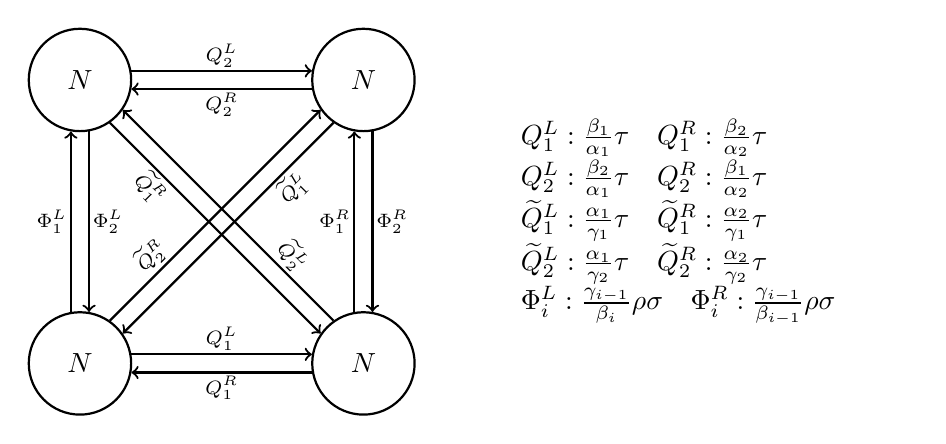
\begin{tikzpicture}[thick,inner sep=0.1em,scale=0.9]
    %gaugenodes  
    \node (L1) at (0,0) [circle,draw,minimum size=1.3cm]{$N$};
    \node (G1) at (4,0) [circle,draw,minimum size=1.3cm]{$N$};
    \node (G2) at (4,-4) [circle,draw,minimum size=1.3cm]{$N$};
    \node (L2) at (0,-4) [circle,draw,minimum size=1.3cm]{$N$};

    \draw [->] (L1.10) -- (G1.170) node[midway,above] {$ \scriptstyle{Q_2^L}$};
    \draw [->] (L2.10) -- (G2.170) node[midway,above] {$\scriptstyle{Q_1^L}$};
    \draw [<-] (L1.350) -- (G1.190) node[midway,below] {$ \scriptstyle{Q_2^R}$};
    \draw [<-] (L2.350) -- (G2.190) node[midway,below] {$\scriptstyle{Q_1^R}$};
    
    \draw [->] (G1.235) -- (L2.35) node[near start,below,sloped] {$\scriptstyle{\widetilde{Q}_1^L}$};
        \draw [<-] (G1.215) -- (L2.55) node[near end,above,sloped] {$\scriptstyle{\widetilde{Q}_2^R}$};
    \draw [->] (G2.125) -- (L1.325) node[near start,above,sloped] {$\scriptstyle{\widetilde{Q}_2^L}$};
        \draw [<-] (G2.145) -- (L1.305) node[near end,below,sloped] {$\scriptstyle{\widetilde{Q}_1^R}$};
    
     \draw [->] (G1.280) -- (G2.80) node[midway,right] {$\scriptstyle{\Phi_2^R}$};
     \draw [<-] (G1.260) -- (G2.100) node[midway,left] {$\scriptstyle{\Phi_1^R}$};
     \draw [->] (L1.280) -- (L2.80) node[midway,right] {$\scriptstyle{\Phi_2^L}$};
     \draw [<-] (L1.260) -- (L2.100) node[midway,left] {$\scriptstyle{\Phi_1^L}$};
     \node at (9,-2) [text width=5cm] {$Q_1^{L}:\frac{\beta_1}{\alpha_1}\tau$\quad $Q_1^R:\frac{\beta_2}{\alpha_2}\tau$\\
   $Q_2^{L}:\frac{\beta_2}{\alpha_1}\tau$\quad $Q_{2}^R:\frac{\beta_1}{\alpha_2}\tau$\\$\widetilde{Q}_1^L:\frac{\alpha_1}{\gamma_1}\tau$\quad $\widetilde{Q}_1^R:\frac{\alpha_2}{\gamma_1}\tau$ \\$\widetilde{Q}_2^L:\frac{\alpha_1}{\gamma_2}\tau$\quad $\widetilde{Q}_2^R:\frac{\alpha_2}{\gamma_2}\tau$\\$\Phi_i^L:\frac{\gamma_{i-1}}{\beta_{i}}\rho\sigma$\quad $\Phi_i^R:\frac{\gamma_{i-1}}{\beta_{i-1}}\rho\sigma$};
 \end{tikzpicture}
  \caption{\it Quiver diagram of the $k=2$ theory associated to a torus with $\ell=2$ minimal punctures.}
  \label{fig:c3z2z2}
\end{figure}
\subsection{Class \texorpdfstring{$\mathcal{S}_k$}{Sk}}
Let us move to the case of general values of $k,\ell$, while again focusing on $N=1$. 
Let's firstly consider $k=\ell=2$. The quiver diagram is given in Figure \ref{fig:c3z2z2}.
Using \textit{Macaulay2} we can compute the Hilbert series for $R/I$. The full moduli space $\mathbf{M}$ is then given as a projection onto gauge invariants
\begin{equation}
\HS(\tau_1,\tau_2,\tau_3;M)=\oint\prod_{A=1}^4\left(\frac{dz_A}{2\pi\iu z_A}\right)f^{\flat}(\tau_1,\tau_2,\tau_3,\alpha,\delta,\gamma,\beta;z_A)\,,
\end{equation}
of the Hilbert series for $\mathbf{F}$
\begin{equation}
\begin{aligned}f^{\flat}=&\frac{z_1z_2z_3z_4P(\tau_1,\tau_2,\tau_3,\alpha,\delta,\gamma,\beta;z_A)}{\left(\beta  \tau _1 z_1-\gamma  z_2\right) \left(\beta  z_1-\gamma  \tau _1 z_2\right) \left(\alpha  \beta  z_1-\tau _3 z_3\right) \left(\beta  \tau _3
   z_1-\delta  z_3\right) }\\
   &\times\frac{1}{ \left(\alpha  \tau _2 z_1-\gamma  z_4\right) \left(z_1-\gamma  \delta  \tau _2 z_4\right) \left(\alpha  \gamma  \tau _2
   z_2-z_3\right) \left(\gamma  z_2-\delta  \tau _2 z_3\right)}\\
   &\times\frac{1}{ \left(\tau _1 z_3-\beta  \gamma z_4\right) \left(z_3-\beta  \gamma  \tau _1 z_4\right)\left(\alpha z_2-\beta  \tau _3 z_4\right) \left(\tau _3 z_2-\beta  \delta  z_4\right)}
 \end{aligned}
\end{equation}
with $P$ polynomial in the $z_A$ and $\tau_{1,2,3}$ and we have set $\gamma=\gamma_1$, $\beta=\beta_1$, $\alpha=\alpha_1$ and $\delta=\alpha_2$. After performing the integrals, we have
\begin{equation}
\begin{aligned}
&\HS(\tau_1,\tau_2,\tau_3;M)=\\&\PE\left[2\tau^2_1+2\tau^2_2+2\tau^2_3\right]\left(\tau _2^2 \tau _3^4 \tau _1^4+\tau _2^2 \tau _1^4+\tau _2^4 \tau _3^2 \tau _1^4-4 \tau _2^2 \tau _3^2 \tau _1^4+\tau _3^2 \tau _1^4\right.\\
&-\tau _2^3 \tau _3^3 \tau _1^3+\tau _2 \tau _3^3 \tau _1^3+\tau
   _2^3 \tau _3 \tau _1^3-\tau _2 \tau _3 \tau _1^3+\tau _2^4 \tau _1^2+\tau _2^4 \tau _3^4 \tau _1^2-4 \tau _2^2 \tau _3^4 \tau _1^2\\
   &+\tau _3^4 \tau _1^2-3 \tau _2^2 \tau _1^2-4 \tau _2^4 \tau _3^2
   \tau _1^2+11 \tau _2^2 \tau _3^2 \tau _1^2-3 \tau _3^2 \tau _1^2+\tau _2^3 \tau _3^3 \tau _1-\tau _2 \tau _3^3 \tau _1\\
   &\left.-\tau _2^3 \tau _3 \tau _1+\tau _2 \tau _3 \tau _1+\tau _2^2 \tau _3^4+\tau _2^4
   \tau _3^2-3 \tau _2^2 \tau _3^2+1\right)\,.
\end{aligned}
\end{equation}
Note that the final expression is independent of $\frac{\alpha}{\delta}$ and both $\gamma$ and $\beta$. This is because for the quivers with $U(N)$ gauge groups the $U(1)$ transformations generated by $q_{\alpha_n\bmod b},q_{\gamma_i},q_{\beta_i}$ are isomorphic to gauge transformations, while for $SU(N)$ gauge groups they are global symmetries. 
As before the Higgs branch is reached by considering the $\tau_1\to0$ limit 
\begin{equation}
\begin{aligned}
&\HS(\tau_2,\tau_3;HB)=\lim_{\tau_1\to0}\HS(\tau_1,\tau_2,\tau_3;M)=\frac{1-3 \tau _3^2 \tau _2^2+\tau _3^2 \tau _2^4+\tau _3^4 \tau _2^2}{\left(1-\tau _2^2\right)^2 \left(1-\tau _3^2\right)^2}\label{eqn:HSU14}\\
&=\PE[\tau_2^2+\tau_3^2]+\PE[2\tau_2^2]+\PE[2\tau_3^2]-\PE[\tau_2^2]-\PE[\tau_3^2]\,.
\end{aligned}
\end{equation}
We notice that the Hilbert series splits into that for $\mathbb{C}^2/(\mathbb{Z}_2\times\mathbb{Z}_2)$ (the mesonic Higgs branch moduli space), and two copies of $(\mathbb{C}/\mathbb{Z}_2)^2$, minus the two common $\mathbb{C}/\mathbb{Z}_2$-line intersections.
From the Plethystic Logarithm 
\begin{equation}
\PLog[\HS(\tau_2,\tau_3;HB)]=2 \tau _2^2+2
   \tau _3^2-3 \tau _3^2 \tau _2^2+\tau _3^2 \tau _2^4+\tau _3^4 \tau _2^2+\dots\,,
\end{equation}
we recognise the generators as $B_i=Q_i^LQ_i^R$, $\widetilde{B}_i=\widetilde{Q}^L_{i}\widetilde{Q}^R_{i+1}$. At the next order we have the relations $B_1\widetilde{B}_1=B_1\widetilde{B}_2=B_2\widetilde{B}_1=B_2\widetilde{B}_2$ thanks to the F-terms $\widetilde{Q}_i^LQ_i^L=Q_{i}^R\widetilde{Q}_{i-1}^R$. The higher order terms are Hilbert syzygies (a.k.a. relations between relations). This should be compared with $\PLog[M(0,\tau_2,\tau_3;\mathbb{C}^2/(\mathbb{Z}_2\times\mathbb{Z}_2))]=\tau_2^2+\tau_3^2$ which is counting only a particular subset of allowed operators.

We can also consider the Coulomb limit
\begin{equation}
\lim_{\tau_2\to0}\lim_{\tau_3\to0}\HS(\tau_1,\tau_2,\tau_3;M)=\HS(T;CB)=\PE\left[2T^2\right]
\end{equation}
corresponding to the operators $\prod_{i=1}^k\Phi_{i}^L$, $\prod_{i=1}^k\Phi^R_{i}$ which indeed have dimension two and have fugacity $\prod_{i=1}^k\frac{\gamma_i}{\beta_{i-1}}=1$ and $\prod_{i=1}^k\frac{\gamma_i}{\beta_{i}}=1$ under the intrinsic symmetries.

For higher values of $k,\ell$ the computations of the Hilbert series become increasingly complex, due to the requirement of making primary decomposition in a larger number of variables using \textit{Macaulay2}. We were able to compute the Higgs-branch Hilbert series for $k=\ell=3$.
\begin{equation}
\HS(\tau_2,\tau_3;HB)=\PE[\tau_2^{3}+\tau_3^{3}]+\PE[3\tau_2^{3}]+\PE[3\tau_3^{3}]-\PE[\tau_2^{3}]-\PE[\tau_3^{3}]
\end{equation}
we note that $\gamma_i$, $\beta_i$ do not appear and $\alpha_n$ enters only via $\alpha_1\alpha_2\alpha_3=b^3$ in the Hilbert series for the Higgs Branch. Moreover, we conjecture that the form of the Hilbert series for arbitrary $k=\ell$ reads
\begin{equation}
\HS(\tau_2,\tau_3;HB)=\PE[\tau_2^{\ell}+\tau_3^{\ell}]+\PE[\ell\tau_2^{\ell}]+\PE[\ell\tau_3^{\ell}]-\PE[\tau_2^{\ell}]-\PE[\tau_3^{\ell}]\,.
\end{equation}
This form for the Hilbert series implies that the moduli space is made up of a copy $\mathbb{C}^2/(\mathbb{Z}_{\ell}\times\mathbb{Z}_{\ell})$, two copies of $(\mathbb{C}/\mathbb{Z}_{\ell})^{\ell}$ minus $\mathbb{C}/\mathbb{Z}_{\ell}$ common intersections.
Importantly, we have that our definition for the Higgs branch, in general, \textit{does not} coincide with the mesonic moduli space $\mathbb{C}^2/(\mathbb{Z}_k\times\mathbb{Z}_{\ell})$. Therefore, in general one cannot obtain the result for general $N$ by simply taking the $N^{\text{th}}$ symmetric product of the $N=1$ result.
\subsubsection{Hall-Littlewood Index}
We can also compute the corresponding Hall-Littlewood index for our theories.
The general expression is given by
\begin{equation}\label{eq:HLlk}
\begin{aligned}
&\HL(\tau_2,\tau_3) =\oint\prod_{n=1}^{\ell}\prod_{i=1}^k\Bigg\{\frac{dz_{n,i}}{2\pi\iu z_{n,i}}\\
&\times\PE\left[\left(\frac{\beta_{i+n-1}}{\alpha_n}\frac{z_{n,i}}{z_{n+1,i}}\tau+\frac{\alpha_n}{\gamma_i}\frac{z_{n+1,i-1}}{z_{n,i}}\tau-\frac{\beta_{i+n-1}}{\gamma_i}\frac{z_{n+1,i-1}}{z_{n+1,i}}\tau^2\right)\right]\Bigg\}\,.
\end{aligned}
\end{equation}
For example, for $k=\ell=2$, $N=1$ we have
\begin{equation}
\textrm{HL}(\tau_2,\tau_3) = \frac{1-4\tau_2^2\tau_3^2+2\tau_2^2\tau_3^4+2\tau_2^4\tau_3^2-\tau_2^4\tau_3^4}{(1-\tau_2^2)^2(1-\tau_3^2)^2}\,.
\end{equation}
For general $\ell=k$ with $N=1$ we were propose the following conjecture, which we checked for various low values of $\ell=k$,
\begin{equation}\label{eqn:HLarbell}
\HL(\tau_2,\tau_3) = \PE[\ell \tau_2^{\ell}]+\PE[\ell \tau_3^\ell]-1\,.
\end{equation}
The ratio $\HL/\HS$ is then counting, with signs, the protected operators of the theory which have $j_1+j_2\geq\frac{1}{2}$ and $r+2j_2=\frac{4}{3}q_t$.

It is possible compute the Hall-Littlewood index for the class $\mathcal{S}_k$ theories with $SU(N)$ gauge groups. For $k=\ell=2$ with $SU(2)^{k\ell}$ gauge group this reads
\begin{equation}
\begin{aligned}
&\HL_{\alpha_1\alpha_2} =\\
&\oint\prod_{n=1}^{\ell}\prod_{i=1}^k\left(\frac{dz_{n,i}}{4\pi\iu z_{n,i}}\frac{\left(1-z_{n,i}^{\pm2}\right)\left(1-\frac{\beta_{i+n-1}}{\gamma_i}\frac{z_{n+1,i-1}^{\pm1}}{z_{n+1,i}^{\pm1}}\tau^2\right)}{\left(1-\frac{\beta_{i+n-1}}{\alpha_n}\frac{z_{n,i}^{\pm1}}{z_{n+1,i}^{\pm1}}\tau\right)\left(1-\frac{\alpha_n}{\gamma_i}\frac{z_{n+1,i-1}^{\pm1}}{z_{n,i}^{\pm1}}\tau\right)}\right)\,.
\end{aligned}
\end{equation}
Expanding and then taking the PLog we have
\begin{equation}
\begin{aligned}
\PLog&\left[\HL_{\alpha_1\alpha_2}\right]=\sum_{i=1}^2\left[\sum_{n=1}^2\left(\frac{\beta_i^2}{\alpha_n ^2}+\gamma_i^2\alpha_n ^2\right)+\left(\frac{1}{\alpha_1  \alpha_2 }+ \alpha_1\alpha_2\right) \right]\tau^2\\
 &+\sum_{n=1}^2\left[\frac{\alpha_n ^2}{\alpha_{n-1} ^2}-\sum_{i=1}^2\frac{\alpha_n}{\alpha_{n-1}}\left(\beta_i^2+\frac{1}{\gamma^{2}_i}\right)-\sum_{i=1}^2\frac{\beta_{i+n-1}^2}{\gamma_{i-1}^2}\right]\tau^4+\mathcal{O}(\tau^6)\,,
\end{aligned}
\end{equation}
recall we also have $\gamma_2=\gamma_1^{-1}$, $\beta_2=\beta_1^{-1}$ and the sums over $i,n$ are taken modulo $k=2$ and $\ell=2$, respectively. The operators with $q_t=1$ correspond to `baryonic type' $\det Q_{i}^{o}$, $\det \widetilde{Q}_{i}^{o}$, with $o=L/R$ and `mesonic type' $\tr Q_{i}^{L}Q_{i}^{R}$ and $\tr \widetilde{Q}_{i}^{L}\widetilde{Q}_{i}^{R}$. At the next order we have bosonic operators $\tr\widetilde{Q}_1^{o}Q_1^{o}\widetilde{Q}_2^{o}Q_2^o$ and fermionic operators of the form $\det Q_i^R\widetilde{Q}_{i-1}^L\overline{\lambda}_j^L$, $\det Q_i^L\widetilde{Q}_{i-1}^R\overline{\lambda}_j^R$ and finally $\tr Q_i^o\widetilde{Q}_{i-1}^o\overline{\lambda}_i^o$. Here $\overline{\lambda}_i^o=\overline{\lambda}^o_{i\dot+}$ denotes fermion in the superfield expansion $\overline{\Phi}^o_i=\overline{\Phi}^o_i+\overline{\theta}^{\dot\alpha}\overline{\lambda}^o_{i\dot\alpha}+\dots$. 

The unrefined $\alpha_n=\gamma_i=\beta_i=1$ limit can be computed exactly and reads
\begin{equation}
\textrm{HL}_{\delta\alpha}=\frac{1+6\tau^2+11\tau^4-12\tau^8-4\tau^{10}}{(1-\tau^2)^6}\,.
\end{equation}

\subsection{Deconstruction Limit}
There have been many precision tests \cite{Hayling:2017cva,Hayling:2018fmv,Hayling:2018fgy,Lambert:2012qy} of the deconstruction proposal \cite{ArkaniHamed:2001ie}. Of most interest to us in this subsection is the fact that \cite{Hayling:2017cva,Bourget:2017sxr} were able to show that the $\frac{1}{2}$-BPS partition function of the $\mathcal{N}=(2,0)$ LST is equal to the Higgs branch Hilbert series of the corresponding 4d $\mathcal{N}=2$ theory in the deconstruction limit. This naturally leads one to expect that a similar story should also exist for the $\mathcal{N}=(1,1)$ LST. The $\mathcal{N}=(1,1)$ LST arises as the worldvolume theory on a stack of $N$ parallel NS5-branes in type IIB string theory \cite{Giveon:1999zm,Aharony:1998ub,Seiberg:1997zk,Berkooz:1997cq,Aharony:1999ks}. 
The basic deconstruction proposal is that the 6d $\mathcal{N}=(1,1)$ LST may be effectively described by considering the $\mathcal{N}=1$ $\mathfrak{u}(N)^{\oplus\ell k}$ toroidal quiver gauge theory realised as the $l_s\to0$ limit of the worldvolume theory on a stack of $N$ D3-branes probing a transverse $\mathbb{C}^3/(\mathbb{Z}_{\ell}\times\mathbb{Z}_k)$ singularity where the quotient acts as in \eqref{eqn:quotientactZkZl}.
We then go to the point in parameter space where the vevs $v_5=\langle Q_{(i,n)}\rangle$, $v_6=\langle \Phi_{(i,n)}\rangle$ (this is a mixed branch in our language) and couplings $G=g^{\text{YM}}_{(i,n)}$ are equal for all nodes in the quiver and then take the limit\footnote{Our parameters are related to those of \cite{ArkaniHamed:2001ie} by $N_5=k$, $N_6=\ell$.}
\begin{equation}
\quad\ell\to\infty\,,\quad k\to\infty\,,\quad G\to\infty\,,\quad v_{5,6}\to\infty\,,\quad 
\end{equation}
while holding $2\pi R_5 Gv_5=\ell$ and $2\pi R_6 Gv_6=k$ fixed. The main point is that, in this limit, the transverse $\mathbb{C}^3/(\mathbb{Z}_{\ell}\times\mathbb{Z}_k)$ can be approximated by $T^2\times\mathbb{R}^4$ where the radii of the torus are $r_{5}=v_5/k$ and $r_6=v_6/\ell$. Performing T-duality along the two circles and then S-duality gives the rank $N$ $\mathcal{N}=(1,1)$ LST on a torus with radii $R_5,R_6$.

Representations of the $\mathcal{N}=(1,1)$ supersymmetry algebra may be decomposed into a finite sum of representations of the bosonic subalgebra given by the sum of Lorentz algebra $\mathfrak{so}(6)$ and R-symmetry algebra $\mathfrak{so}(4)\iso\mathfrak{su}(2)_{R_1}\oplus \mathfrak{su}(2)_{R_2}$. The supercharges sit in the representations $\Qsix\in[0,1,0]^{\left(\frac{1}{2},0\right)}_{\frac{1}{2}}$ and $\widetilde{\Qsix}\in[0,0,1]^{\left(0,\frac{1}{2}\right)}_{\frac{1}{2}}$ with representations labelled by $[h_1,h_2,h_3]_E^{(R_1,R_2)}$. In other words $\Qsix_{h_1h_2h_3}^a$ with $h_i=\pm\frac{1}{2}$ such that $8h_1h_2h_3=-1$ and $\widetilde{\Qsix}_{h_1h_2h_3}^{\dot a}$ with $8h_1h_2h_3=+1$. They obey
\begin{equation}
\{\Qsix^a,\Qsix^b\}=\epsilon^{ab}\eta^{\mu}p_{\mu}\,,\quad\{\widetilde{\Qsix}^{\dot a},\widetilde{\Qsix}^{\dot b}\}=\epsilon^{\dot a\dot b}\widetilde{\eta}^{\mu}p_{\mu}\,,\quad\{\Qsix^{ a},\widetilde{\Qsix}^{\dot b}\}=0\,,
\end{equation}
where $\eta^{\mu},\widetilde{\eta}^{\mu}$, $\mu=1,2,\dots,6$ denote the `t Hooft symbols which intertwine between $\mathfrak{su}(4)$ and $\mathfrak{so}(6)$. The 4d $\mathcal{N}=1$ supersymmetry algebra plus the residual global  $\mathfrak{u}(1)_t\oplus\mathfrak{u}(1)_b$ symmetry algebras can be embedded into the 6d $\mathcal{N}=(1,1)$ algebra with the relations\footnote{These can be obtained in the following way: the first two relations are simply the identifications one would make between the Cartans for $\mathfrak{su}(2)_1\oplus\mathfrak{su}(2)_2\iso\mathfrak{so}(4)\subset\mathfrak{so}(6)$. When compactifying the 6d theory on $T^2$ the spinor label $h_1$  $h_1=H=H_R+H_L$ on $T^2$ and $2H_L=q_1$, $2H_R=q_2$. Finally $2R_2=q_1-q_2$ is fixed by demanding that $R_2$ evaluates to zero on the $\mathcal{N}=1$ subsector. This then fixes $q_3=R_1$. The identifications \eqref{eqn:N4N1ides} then give \eqref{eqn:6dembedding}.}
\begin{gather}
2j_1=h_2+h_3\,,\quad 2j_2=h_2-h_3\,,\\
\frac{3}{2}r=2h_1+R_1\,,\quad 2q_t=-h_1+R_1-3R_2\,,\quad q_b=h_1-R_1-R_2\label{eqn:6dembedding}\,.
\end{gather}
The relationship between the 4d and 6d supercharges is given in Table \ref{tab:6d4dembedding}.
\begin{table}
\centering
\begin{tabular}{|c|c|c|c|c|c|c|} 
\hline
 6d $\mathcal{N}=(1,1)$&  $(h_1,h_2,h_3,R_1,R_2)$ & $(j_1,j_2)$ & $r$ &$q_t$&$q_b$& 4d $\mathcal{N}=1$\\ 
 \hline\hline
 $\Qsix^{1}_{+\pm\mp}$&$(+\frac{1}{2},\pm\frac{1}{2},\mp\frac{1}{2},+\frac{1}{2},0)$&$(0,\pm\frac{1}{2})$&$+1$&$0$&$0$&$\widetilde{\mathcal{Q}}_{\dot\pm}$\\\hline
   $\Qsix^{1}_{-\pm\pm}$&$(-\frac{1}{2},\pm\frac{1}{2},\mp\frac{1}{2},+\frac{1}{2},0)$&$(\pm\frac{1}{2},0)$&$-\frac{1}{3}$&$1$&$-1$&\\\hline
 $\Qsix^{2}_{+\pm\mp}$&$(+\frac{1}{2},\pm\frac{1}{2},\mp\frac{1}{2},-\frac{1}{2},0)$&$(0,\pm\frac{1}{2})$&$+\frac{1}{3}$&$-1$&$+1$&\\\hline
    $\Qsix^{2}_{-\pm\pm}$&$(-\frac{1}{2},\pm\frac{1}{2},\pm\frac{1}{2},-\frac{1}{2},0)$&$(\pm\frac{1}{2},0)$&$-1$&$0$&$0$&$\mathcal{Q}_{\pm}$\\\hline
$\widetilde{\Qsix}^{\dot1}_{+\pm\pm}$&$(+\frac{1}{2},\pm\frac{1}{2},\pm\frac{1}{2},0,+\frac{1}{2})$&$(\pm\frac{1}{2},0)$&$+\frac{2}{3}$&$-1$&$0$&\\\hline
$\widetilde{\Qsix}^{\dot1}_{-\pm\mp}$&$(-\frac{1}{2},\pm\frac{1}{2},\mp\frac{1}{2},0,+\frac{1}{2})$&$(0,\pm\frac{1}{2})$&$-\frac{2}{3}$&$-\frac{1}{2}$&$-1$&\\\hline
$\widetilde{\Qsix}^{\dot2}_{+\pm\pm}$&$(+\frac{1}{2},\pm\frac{1}{2},\pm\frac{1}{2},0,-\frac{1}{2})$&$(\pm\frac{1}{2},0)$&$+\frac{2}{3}$&$+\frac{1}{2}$&$+1$&\\\hline
$\widetilde{\Qsix}^{\dot2}_{-\pm\mp}$&$(-\frac{1}{2},\pm\frac{1}{2},\mp\frac{1}{2},0,-\frac{1}{2})$&$(0,\pm\frac{1}{2})$&$-\frac{2}{3}$&$+1$&$0$&\\\hline
\end{tabular}
\caption{\textit{One choice of embedding of the 4d $\mathcal{N}=1$ superalgebra into the 6d $\mathcal{N}=(1,1)$ superalgebra.}}
\label{tab:6d4dembedding}
\end{table}

Let us now move to our candidate set of operators on the 4d side that will ultimately reproduce the $\frac{1}{2}$-BPS scalar operators in the $(1,1)$ LST.
Let's assume that, after primary decomposition, we can always identify a irreducible branch ${}^{\text{mes}}\mathbf{M}=\mathbf{M}//U(1)_D$ inside the full moduli space $\mathbf{M}$. ${}^{\text{mes}}\mathbf{M}$ will be our candidate for reproducing the 6d $\frac{1}{2}$-BPS ring. For any $\mathcal{N}=1$ theory, the operators parametrising $\mathbf{M}$ are themselves $\frac{1}{2}$-BPS with respect to the $\mathcal{N}=1$ supersymmetry algebra, namely they are annihilated by $\widetilde{\mathcal{Q}}_{\dot\alpha}$. 

One may wonder why we have picked the subvariety ${}^{\text{mes}}\mathbf{M}$ as opposed to the full moduli space $\mathbf{M}$. Shortly we will prove that that, for the theory with $U(N)$ gauge groups, in the $k,\ell\to\infty$ limit that ${}^{\text{mes}}\mathbf{M}$ coincides with $\mathbf{M}$.

Let us first focus on the $N=1$ case. We can set, without loss of generality in this limit, $k=\ell$. The possible gauge invariant operators parametrising $\mathbf{M}$ for the theory with $U(1)$ gauge groups are in correspondence with the number of closed, directed paths that one can draw on the quiver diagram.  There are four main types of operators. There are those which involve an equal number $p\leq k=\ell$ of $Q$, $\widetilde{Q}$ and $\Phi$ fields. Such an operator enters the Hilbert series with fugacity $\tau_1^p\tau_2^p\tau_3^p$. Operators of this form correspond to picking a base node, say $(i=1,n=1)$, and drawing a closed loop involving $p$ vertical steps, $p$ horizontal steps and $p$ diagonal steps. However, recall the F-terms set
\begin{equation}
\label{eqn:PhiF}F_{\Phi_{(i,n)}}=\widetilde{Q}_{(i,n-1)}Q_{(i,n-1)}-Q_{(i-1,n)}\widetilde{Q}_{(i,n)}=0\,,
\end{equation}
\begin{equation}
\label{eqn:QF}F_{Q_{(i,n)}}=\Phi_{(i,n+1)}\widetilde{Q}_{(i,n)}-\widetilde{Q}_{(i+1,n)}\Phi_{(i+1,n)}=0\,,
\end{equation}
\begin{equation}
\label{eqn:QtF}F_{\widetilde{Q}_{(i,n)}}=Q_{(i,n)}\Phi_{(i,n+1)}-\Phi_{(i,n)}Q_{(i-1,n)}=0\,.
\end{equation}
In terms of the quiver diagram Figure \ref{fig:Skquivergenus1}, this means that the operations of moving right, up or diagonally all commute. In other words this means that the associated operator is independent of the choice of base node and of the specific path chosen, it depends only on the length $3p$. See Figure \ref{fig:pathexample} for a diagrammatic example for $p=3$. In that example on the left we have the operator \newline$Q_{(i,n)}Q_{(i,n+1)}Q_{(i,n+2)}\Phi_{(i,n+3)}\Phi_{(i-1,n+3)}\widetilde{Q}_{(i-1,n+2)}\Phi_{(i-1,n+2)}\widetilde{Q}_{(i-1,n+1)}\widetilde{Q}_{(i,n)}$ which is reduced to $\prod_{m=0}^2 Q_{(i,n+m)}\Phi_{(i,n+m+1)}\widetilde{Q}_{(i,n+m)}$. Again further applying the F-terms means this operator can be written simply as $m^p=m^3$ with, say, $m=\widetilde{Q}_{(1,\ell)}Q_{(1,\ell)}\Phi_{(1,1)}$.
\begin{figure}
\centering
\begin{subfigure}[t]{0.45\textwidth}
\centering
  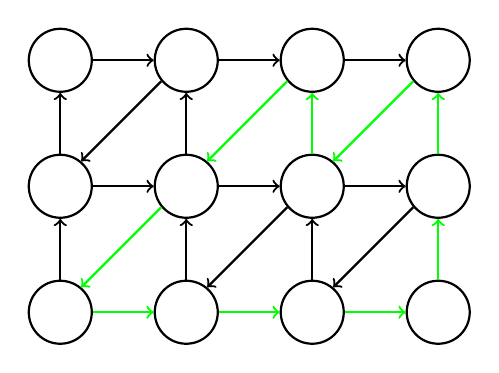
\begin{tikzpicture}[square/.style={regular polygon,regular polygon sides=4},thick,inner sep=0.1em,scale=0.8]
    \node (G11) at (0,0)[circle,draw,minimum size=0.8cm]{};
    \node (G21) at (2,0) [circle,draw,minimum size=0.8cm]{};
    \node (G31) at (4,0) [circle,draw,minimum size=0.8cm]{};
    \node (G41) at (6,0) [circle,draw,minimum size=0.8cm]{};
    \node (G12) at (0,-2)[circle,draw,minimum size=0.8cm]{};
    \node (G22) at (2,-2) [circle,draw,minimum size=0.8cm]{};
    \node (G32) at (4,-2) [circle,draw,minimum size=0.8cm]{};
    \node (G42) at (6,-2)[circle,draw,minimum size=0.8cm]{};
	\node (G13) at (0,-4)[circle,draw,minimum size=0.8cm]{};
    \node (G23) at (2,-4) [circle,draw,minimum size=0.8cm]{};
    \node (G33) at (4,-4) [circle,draw,minimum size=0.8cm]{};
    \node (G43) at (6,-4)[circle,draw,minimum size=0.8cm]{};
    
    \draw [<-] (G11.270) to (G12.90);
    \draw [<-] (G21.270) to (G22.90);
    \draw [<-,color=green] (G31.270) to (G32.90);
    \draw [<-,color=green] (G41.270) to (G42.90);
    \draw [<-] (G12.270) to (G13.90);
    \draw [<-] (G22.270) to (G23.90);
    \draw [<-] (G32.270) to (G33.90);
    \draw [<-,color=green] (G42.270) to (G43.90);
   
    \draw [->](G11.0) to (G21.180);
    \draw [->] (G21.0) to (G31.180);
    \draw [->] (G31.0) to (G41.180);
    \draw [->] (G12.0) to (G22.180);
    \draw [->] (G22.0) to (G32.180);
    \draw [->] (G32.0) to (G42.180);
    \draw [->,color=green] (G13.0) to (G23.180);
    \draw [->,color=green] (G23.0) to (G33.180);
    \draw [->,color=green] (G33.0) to (G43.180);

	\draw [<-,color=green] (G13.50) to (G22.220);
    \draw [<-] (G23.50) to (G32.220);
    \draw [<-] (G33.50) to (G42.220);
    \draw [<-,color=green] (G32.50) to (G41.220);
    \draw [<-,color=green] (G22.50) to (G31.220);
    \draw [<-] (G12.50) to (G21.220);
  \end{tikzpicture}
  \end{subfigure}\quad
  \begin{subfigure}[t]{0.45\textwidth}
  \centering
    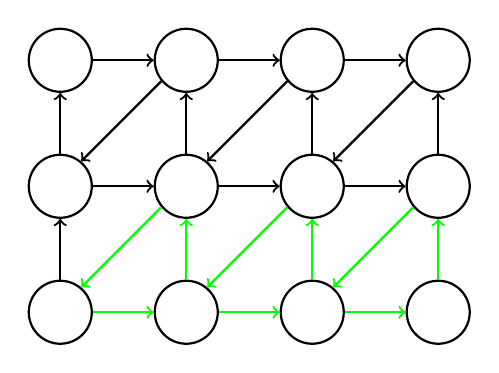
\begin{tikzpicture}[square/.style={regular polygon,regular polygon sides=4},thick,inner sep=0.1em,scale=0.8]
    %gaugenodes
    \node (G11) at (0,0)[circle,draw,minimum size=0.8cm]{};
    \node (G21) at (2,0) [circle,draw,minimum size=0.8cm]{};
    \node (G31) at (4,0) [circle,draw,minimum size=0.8cm]{};
    \node (G41) at (6,0) [circle,draw,minimum size=0.8cm]{};
    \node (G12) at (0,-2)[circle,draw,minimum size=0.8cm]{};
    \node (G22) at (2,-2) [circle,draw,minimum size=0.8cm]{};
    \node (G32) at (4,-2) [circle,draw,minimum size=0.8cm]{};
    \node (G42) at (6,-2)[circle,draw,minimum size=0.8cm]{};
	\node (G13) at (0,-4)[circle,draw,minimum size=0.8cm]{};
    \node (G23) at (2,-4) [circle,draw,minimum size=0.8cm]{};
    \node (G33) at (4,-4) [circle,draw,minimum size=0.8cm]{};
    \node (G43) at (6,-4)[circle,draw,minimum size=0.8cm]{};
    
    %down chirals phi1
    \draw [<-] (G11.270) to (G12.90);
    \draw [<-] (G21.270) to (G22.90);
    \draw [<-] (G31.270) to (G32.90);
    \draw [<-] (G41.270) to (G42.90);
    \draw [<-] (G12.270) to (G13.90);
    \draw [<-,color=green] (G22.270) to (G23.90);
    \draw [<-,color=green] (G32.270) to (G33.90);
    \draw [<-,color=green] (G42.270) to (G43.90);
    
    %right phi2
    \draw [->](G11.0) to (G21.180);
    \draw [->] (G21.0) to (G31.180);
    \draw [->] (G31.0) to (G41.180);
    \draw [->] (G12.0) to (G22.180);
    \draw [->] (G22.0) to (G32.180);
    \draw [->] (G32.0) to (G42.180);
    \draw [->,color=green] (G13.0) to (G23.180);
    \draw [->,color=green] (G23.0) to (G33.180);
    \draw [->,color=green] (G33.0) to (G43.180);

	\draw [<-,color=green] (G13.50) to (G22.220);
    \draw [<-,color=green] (G23.50) to (G32.220);
    \draw [<-,color=green] (G33.50) to (G42.220);
    \draw [<-] (G32.50) to (G41.220);
    \draw [<-] (G22.50) to (G31.220);
    \draw [<-] (G12.50) to (G21.220);
  \end{tikzpicture}
  \end{subfigure}
  \caption{\it Visualisation for the example of $p=3$.}
  \label{fig:pathexample}
\end{figure}
We can therefore write these operators as $m^p$. The other types of operators involve only $Q$'s, $\widetilde{Q}$'s or $\Phi$'s. They can be written as powers of
\begin{equation}
B_{\Phi_n}=\prod_{i=1}^{\ell}\Phi_{(i,n)}\,,\quad B_{Q_i}=\prod_{n=1}^{\ell}Q_{(i,n)}\,,\quad B_{\widetilde{Q}_i}=\prod_{j=1}^{\ell}\widetilde{Q}_{(i+j,i-j)}\,,
\end{equation}
they enter the Hilbert series with fugacity $\tau_1^{\ell}$, $\tau_2^{\ell}$ and $\tau_3^{\ell}$, respectively. In degree $\geq\min(k,\ell)$ there can be complicated relations and higher syzgies between $m$, $B_{Q_i}$, $B_{\widetilde{Q}_i}$ and $B_{\Phi_n}$, leading to a complicated structure for $\mathbf{M}$. However, the main point is that in the $\ell=k\to\infty$ limit the $B_{Q_i}$, $B_{\widetilde{Q}_i}$ and $B_{\Phi_n}$ operators all become infinity heavy and their dimensions $E=k=\ell$ tend to infinity, in particular $\lim_{\ell\to\infty}\tau_{1,2,3}^{\ell}\to0$ and their contribution to the Hilbert series vanishes. This also implies that the corresponding ring becomes freely generated, since there are no relations between the operators in degree smaller than $\min(k,\ell)\to\infty$. Only the dimension of $m$ remains finite in the limit. $m$ is a purely mesonic operator and therefore, in this limit, one indeed expects ${}^{\text{mes}}\mathbf{M}$ to coincide with $\mathbf{M}$. 

The above arguments can be simply extended to the case $N\geq2$ by taking traces. Each path with an equal number $p$ of $Q$, $\widetilde{Q}$ and $\Phi$'s now corresponds to $A=1,\dots,N$ operators of dimension $3pA$ corresponding to operators schematically of the form $\tr (Q^p\widetilde{Q}^p\Phi^p)^A$. As long as we consider the traces we can apply the same rules that we did for $N=1$, namely that the operations of moving right, up or diagonally commute. This again means any path of length $3p$ can be written as the loop given by $m^p$ with, say, $m=\widetilde{Q}_{(1,\ell)}Q_{(1,\ell)}\Phi_{(1,1)}$ which is now a $N\times N$ matrix. The $N$ operators corresponding to one of these closed paths can then be written  as $m_{(A)}^p$ with
\begin{equation}
m_{(A)}:=\tr m^A=\tr\left(\widetilde{Q}_{(1,\ell)}Q_{(1,\ell)}\Phi_{(1,1)}\right)^A\,.
\end{equation}
As before the $m_{(A)}$ can have complicated relations with the operators which are of the form $\tr B_{Q_i}^A$, $\tr B_{\widetilde{Q}_i}^A$ and $\tr B^A_{\Phi_i}$ but the dimensions of the latter are $Ak=A\ell\to\infty$. 

We therefore arrive at the conclusion that, in the deconstruction $k,\ell\to\infty$ limit $\mathbf{M}$ coincides with ${}^{\text{mes}}\mathbf{M}$ for all $N$.

For the $N=1$ case we can identify ${}^{\text{mes}}\mathbf{M}=\mathbb{C}^3/(\mathbb{Z}_{\ell}\times\mathbb{Z}_k)$, so the Hilbert series for the $N=1$ case is given by \eqref{eqn:moilen}. Therefore, the Hilbert series for general $N$ is given by
\begin{equation}
\label{eq:hsg}
N!\HS(\tau_1,\tau_2,\tau_3;{}^{\text{mes}}M) = \frac{\partial^{N}}{\partial\nu^{N}}\left.\PE\left[\nu M(\tau_1,\tau_2,\tau_3;\mathbb{C}^3/(\mathbb{Z}_{\ell}\times\mathbb{Z}_k))\right]\right|_{\nu=0}\, .
\end{equation}
Let us now consider the deconstruction limit. Taking the limit on the $N=1$ result, recalling that $|\tau_{1,2,3}|<1$, gives
\begin{equation}
\begin{aligned}
&\lim_{k,\ell\to\infty}M(\tau_1,\tau_2,\tau_3;\mathbb{C}^3/(\mathbb{Z}_{\ell}\times\mathbb{Z}_k))\\
&=\lim_{k\to\infty}\PE\left[\tau_1\tau_2\tau_3+\tau_1^k+\tau_2^k\tau_3^k-\tau_1^k\tau_2^k\tau_3^k\right]=\PE\left[\tau_1\tau_2\tau_3\right]=\PE[pq]\,.
\end{aligned}
\end{equation}
Therefore, for general $N$, we have
\begin{equation}\label{eqn:decon4d}
\lim_{\ell,k \to\infty}\HS(\tau_1,\tau_2,\tau_3;{}^{\text{mes}}M)= \PE\left[\sum_{p=1}^{N}(\tau_1\tau_2\tau_3)^{p}\right]=\frac{1}{(\tau_1\tau_2\tau_3;\tau_1\tau_2\tau_3)_N} \, .
\end{equation}
The coordinate-ring of $\mathbf{M}$ for this theory in the $k,\ell\to\infty$ limit is therefore simply $M=\mathbb{C}[m_{(1)},m_{(2)},\dots,m_{(N)}]$.
\subsubsection{Computation of the $\frac{1}{2}$-BPS Partition Function for $(1,1)$ LST}
Let us now move to the computation of the 6d quantity that we would like to match to the 4d quantity \eqref{eqn:decon4d}. We can use the fact that, at low energies, the $\mathcal{N}=(1,1)$ LST admits an effective description as 6d maximally supersymmetric SYM theory with gauge group $U(N)$.  
The on-shell degrees of freedom of the $(1,1)$ SYM theory contains a 2-form gauge field strength $F\in[0,1,1]_{2}^{(0,0)}$, scalars $X\in[0,0,0]_{2}^{(\frac{1}{2},\frac{1}{2})}$ and fermions $\lambda\in[0,1,0]_{\frac{5}{2}}^{(0,\frac{1}{2})}$, $\widetilde{\lambda}\in[0,0,1]_{\frac{5}{2}}^{(\frac{1}{2},0)}$ all in the adjoint of $\mathfrak{g}=\mathfrak{u}(N)$.
The supersymmetry transformations of interest to us are
\begin{equation}
\Qsix^{a}X^{b\dot b}=\frac{1}{\sqrt{2}}\epsilon^{ab}\lambda^{\dot b}\,,\quad \widetilde{\Qsix}^{\dot a}X^{b \dot b}=\frac{1}{\sqrt{2}}\epsilon^{\dot a \dot b}\widetilde{\lambda}^{b}\,.
\end{equation}
We can therefore construct $\frac{1}{2}$-BPS multiplets whose highest weight state is annihilated by both $\Qsix^1$ and $\widetilde{\Qsix}^{\dot1}$. The supersymmetric primary of these multiplets is given by
\begin{equation}
\mathcal{O}_A:=\tr\left(X^{1\dot1}\right)^A
\end{equation}
which are independent for $A=1,\dots,N$. These have
\begin{equation}
\text{$h_1=h_2=h_3=0$ and $E=4R_1=4R_2=2A$}\,.
\end{equation}
By acting with all possible supersymmetries $\Qsix,\widetilde{\Qsix}$ and $\mathfrak{so}(6)\oplus\mathfrak{su}(2)_{R_1}\oplus\mathfrak{su}(2)_{R_2}$ generators we can generate the entire $\frac{1}{2}$-BPS multiplet by acting on the highest weight state $\mathcal{O}_A$.
We can define a $\frac{1}{2}$-BPS partition function (Hilbert series) by passing to the scalar sector of the $\Qsix^1\cap\widetilde{\Qsix}^{\dot1}$ -cohomology
\begin{gather}\label{eqn:1comma1BPS}
Z^{(1,1)}_{\text{$\frac{1}{2}$-BPS}}=\Tr_{\mathcal{H}}x^{2R_1}\,,\\ \mathcal{H}=\left\{\mathbb{C}[\mathbf{\mathcal{O}}]^{\mathfrak{g}}\middle|E=4R_1=4R_2\,,h_1=h_2=h_3=0\right\}\,.
\end{gather}
With this definition we have constructed an object which is counting only the gauge invariant words comprised of scalar component $X^{1\dot1}$ in the $(1,1)$ SYM theory. Using letter counting we can compute
\begin{equation}
Z^{(1,1)}_{\text{$\frac{1}{2}$-BPS}}=\oint d\mu_{U(N)}\PE\left[x\,\chi_{\text{adj}}(\mathbf{z})\right]=\frac{1}{(x;x)_N}\,,
\end{equation}
this is the Hilbert series for $\mathbb{C}[\mathcal{O}_1,\mathcal{O}_2,\dots,\mathcal{O}_N]$. Identifying $x=\tau_1\tau_2\tau_3=pq$ we have matched $Z^{(1,1)}_{\text{$\frac{1}{2}$-BPS}}$ with \eqref{eqn:decon4d} and the map between the operators is just
\begin{equation}
m_{(A)}\xleftrightarrow[]{\text{4d:6d}}\mathcal{O}_A\,.
\end{equation}
These operators can be expected to be found as a subset of those counted by the $\mathbb{S}^1\times \mathbb{S}^5$ partition function. By the Nahm classification \cite{Nahm:1977tg}, there is no superconformal algebra associated to $\mathcal{N}=(1,1)$ SUSY in 6d so there is no superconformal index associated to this theory nevertheless we can define the $\mathbb{S}^1\times \mathbb{S}^5$ partition function of the theory
\begin{equation}\label{eqn:ZLST}
Z^{(1,1)}_{\mathbb{S}^1\times \mathbb{S}^5}(x,y,p_1,p_2)\propto\Tr_{\mathbb{S}^5}(-1)^Fe^{-\beta H}x^{E-R_1}y^{R_2}p_1^{h_1-h_3}p_2^{h_2-h_3}
\end{equation}
where $H=\{\Qsix,\Qsix^{\dagger}\}=E-h_1-h_2-h_3-4R_1$ with $\Qsix:=\Qsix_{---}^{1}$. The partition function \eqref{eqn:ZLST} can be computed using the elliptic genus method \cite{Kim:2015gha,Kim:2017xan,Kim:2018gak} or using the refined topological string \cite{Iqbal:2007ii,Lockhart:2012vp}. $Z^{(1,1)}_{\mathbb{S}^1\times \mathbb{S}^5}$ is expected to receive both perturbative contributions aswell as non-perturbative contributions from 6d SYM instanton string states.

If we consider taking $xy=p_1=p_2=1$ then
\begin{equation}\label{eqn:ZLSTunref}
Z^{(1,1)}_{\mathbb{S}^1\times \mathbb{S}^5}(x,x^{-1},1,1)\propto\Tr_{\mathbb{S}^5}(-1)^Fe^{-\beta H}x^{E-R_1-R_2}
\end{equation}
receives extra shortening and is annihilated by $\Qsix$ and $\widetilde{\Qsix}_{+--}^{\dot1}$ ,$\widetilde{\Qsix}_{-+-}^{\dot1}$, $\widetilde{\Qsix}_{--+}^{\dot1}$. Therefore the unrefined limit \eqref{eqn:ZLSTunref} receives non-zero contributions only from states with $h_1=h_2=h_3=E-4R_2$ and $E+2R_1=6R_2$. $\mathcal{H}$ is clearly contained as a subset of those states when $E=4R_2$. 

We also note that \eqref{eqn:1comma1BPS} is equal to the $\frac{1}{2}$-BPS limit of the index of the $\mathcal{N}=(2,0)$ theory of type $\mathfrak{g}=\mathfrak{u}(N)$, which we have computed in \eqref{eqn:12bps6dpart}. Our result therefore falls into the general result that, in all known examples, the $\frac{1}{2}$-BPS partition function seems to be a universal quantity in all maximally supersymmetric theories in $3$, $4$ and $6$ dimensions \cite{Kim:2016usy}. Additionally, 
the $(1,1)$ and $(2,0)$ LSTs are related by T-duality. T-duality exchanges winding and momentum modes along the temporal $\mathbb{S}^1$. Since, by definition, $Z^{(1,1)}_{\text{$\frac{1}{2}$-BPS}}$ and the analogous quantity $Z^{(2,0)}_{\text{$\frac{1}{2}$-BPS}}$ \cite{Bhattacharyya:2007sa,Kim:2013nva} defined for the $(2,0)$ theory count operators only in the zero winding and zero momentum sectors one naturally expects $Z^{(1,1)}_{\text{$\frac{1}{2}$-BPS}}=Z^{(2,0)}_{\text{$\frac{1}{2}$-BPS}}$.
It would be interesting to further investigate if it is possible to obtain the more general partition functions, such as \eqref{eqn:ZLST} and \eqref{eqn:ZLSTunref}, from 4d class $\mathcal{S}_k$ quantities using deconstruction \cite{Hayling:2017cva,Hayling:2018fmv,Hayling:2018fgy}.


\section{Interacting Trinion SCFTs}
\begin{figure}
\centering
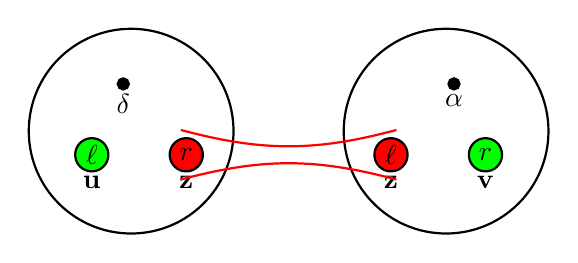
\begin{tikzpicture}[thick]
  \draw (0,0) ellipse (1.3cm and 1.3cm);
  \draw (4,0) ellipse (1.3cm and 1.3cm);
  \node (LU) at (0.5,0.05) {};
  \node (LD) at (0.5,-0.65) {};
  \node (RU) at (3.5,0.05) {};
  \node (RD) at (3.5,-0.65) {};
  \draw [black,fill=black] (-0.1,0.6) circle (2pt) node [below]{$\delta$};
  \draw [black,fill=black] (4.1,0.6) circle (2pt) node [below]{$\alpha$};
  \draw [black,fill=green] (-0.5,-0.3) circle (6pt) node [below=4pt]{$\mathbf{u}$} node{$\ell$};
  \draw [black,fill=green] (4.5,-0.3) circle (6pt) node [below=4pt]{$\mathbf{v}$} node {$r$};
  \draw [black,fill=red] (3.3,-0.3) circle (6pt) node [below=4pt]{$\mathbf{z}$} node {${\ell}$};
  \draw [black,fill=red] (0.7,-0.3) circle (6pt) node [below=4pt]{$\mathbf{z}$} node {$r$};
 \draw [red](LU) to [bend right=15] (RU); 
 \draw [red](LD) to [bend left=15] (RD);
\end{tikzpicture}\\
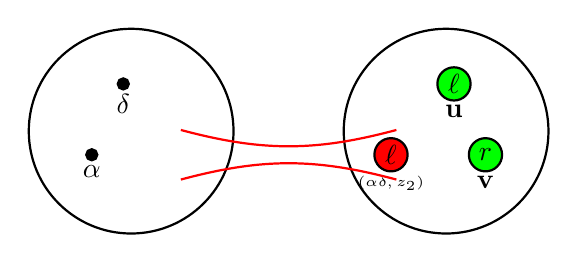
\begin{tikzpicture}[thick]
  \draw (0,0) ellipse (1.3cm and 1.3cm);
  \draw (4,0) ellipse (1.3cm and 1.3cm);
  \node (LU) at (0.5,0.05) {};
  \node (LD) at (0.5,-0.65) {};
  \node (RU) at (3.5,0.05) {};
  \node (RD) at (3.5,-0.65) {};
  \draw [black,fill=black] (-0.1,0.6) circle (2pt) node [below]{$\delta$};
  \draw [black,fill=green] (4.1,0.6) circle (6pt) node [below=4pt]{$\mathbf{u}$} node {$\ell$};
  \draw [black,fill=black] (-0.5,-0.3) circle (2pt) node [below]{$\alpha$};
  \draw [black,fill=green] (4.5,-0.3) circle (6pt) node [below=4pt]{$\mathbf{v}$} node {$r$};
  \draw [black,fill=red] (3.3,-0.3) circle (6pt) node [below=4pt]{\tiny $ (\alpha\delta,z_2)$} node {$\ell$};
 \draw [red] (LU) to [bend right=15] (RU); 
 \draw [red](LD) to [bend left=15] (RD);
\end{tikzpicture}\\
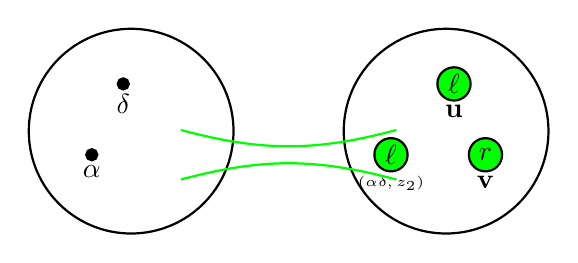
\begin{tikzpicture}[thick]
  \draw (0,0) ellipse (1.3cm and 1.3cm);
  \draw (4,0) ellipse (1.3cm and 1.3cm);
  \node (LU) at (0.5,0.05) {};
  \node (LD) at (0.5,-0.65) {};
  \node (RU) at (3.5,0.05) {};
  \node (RD) at (3.5,-0.65) {};
  \draw [black,fill=black] (-0.1,0.6) circle (2pt) node [below]{$\delta$};
  \draw [black,fill=green] (4.1,0.6) circle (6pt) node [below=4pt]{$\mathbf{u}$} node {$\ell$};
  \draw [black,fill=black] (-0.5,-0.3) circle (2pt) node [below]{$\alpha$};
  \draw [black,fill=green] (4.5,-0.3) circle (6pt) node [below=4pt]{$\mathbf{v}$} node {$r$};
  \draw [black,fill=green] (3.3,-0.3) circle (6pt) node [below=4pt]{\tiny $ (\alpha\delta,z_2)$} node {$\ell$};
 \draw [green](LU) to [bend right=15] (RU); 
 \draw [green](LD) to [bend left=15] (RD);
\end{tikzpicture}
\caption{\textit{Three `S-dual' frames of the basic $A_1$ four punctured sphere in class $\mathcal{S}_2$. On the top is the canonical weakly coupled frame with fluxes for $U(1)_{\beta}\times U(1)_{\gamma}\times U(1)_t$ given by $\mathcal{F}=(0,0,1)$. In the middle is the S-dual frame obtained by gluing a quiver tail to the $T_B$ theory with flux $\mathcal{F}_B=(-\frac{1}{4},\frac{1}{4},1)$. On the bottom is the S-dual frame obtained by gluing a quiver tail to the $T_A$ theory with fluxes $\mathcal{F}_A=(\frac{1}{4},\frac{1}{4},1)$. Green (red) circles indicate maximal punctures of colour $c=0$ ($c=1$). $o=l,r$ indicates the orientation of a maximal puncture. Dots indicate minimal punctures.}}
\label{fig:sduals}
\end{figure}
\begin{figure}
\centering
\begin{tikzpicture}[square/.style={regular polygon,regular polygon sides=4},thick,inner sep=0.1em,scale=0.9]
    %gaugenodes  
    \node (L1) at (0,0) [square,draw,minimum size=1.8cm]{$u_1$};
    \node (R1) at (10,0) [square,draw,minimum size=1.8cm]{$v_2$};
    \node (G1) at (5,0) [circle,draw,minimum size=1.3cm]{$b$};
    \node (G2) at (5,-3) [circle,draw,minimum size=1.3cm]{$a$};
    \node (L2) at (0,-3) [square,draw,minimum size=1.8cm]{$u_2$};
    \node (R2) at (10,-3) [square,draw,minimum size=1.8cm]{$v_1$};

    \draw [->] (L1.0) -- (G1.180) node[midway,above] {$ \scriptstyle{Q^-_{1}\,,\,\delta\gamma\sqrt{t}}$};
    \draw [->] (L2.0) -- (G2.180) node[midway,below] {$\scriptstyle{Q_2^-\,,\,\frac{\delta}{\gamma}\sqrt{t}}$};
    \draw [->] (G1.0) -- (R1.180) node[midway,above] {$\scriptstyle{{Q'_2}^+\,,\,\frac{\alpha}{\gamma}\sqrt{t}}$};
    \draw [->] (G2.0) -- (R2.180) node[midway,below] {$\scriptstyle{{Q'_1}^+\,,\,\alpha\gamma\sqrt{t}}$};
    
    \draw [->] (G1.225) -- (L2.45) node[near start,above,sloped] {$\scriptstyle{Q_2^+\,,\,\frac{1}{\delta\beta}\sqrt{t}}$};
       \draw [->] (R1.225) -- (G2.45) node[near end,below,sloped] {$\scriptstyle{{Q'_2}^-\,,\,\frac{1}{\alpha\beta}\sqrt{t}}$};
    \draw [->] (G2.135) -- (L1.315) node[near start,below,sloped] {$\scriptstyle{Q_1^+\,,\,\frac{\beta}{\delta}\sqrt{t}}$};
    \draw [->] (R2.135) -- (G1.315) node[near end,above,sloped] {$\scriptstyle{{Q'_1}^-\,,\,\frac{\beta}{\alpha}\sqrt{t}}$};
    
     \draw [<-] (G1.280) -- (G2.80) node[midway,right] {$\scriptstyle{\Phi_2\,,\,\gamma\beta\frac{pq}{t}}$};
     \draw [->] (G1.260) -- (G2.100) node[midway,left] {$\scriptstyle{\Phi_1\,,\,\frac{1}{\gamma\beta}\frac{pq}{t}}$};
         
 \end{tikzpicture}
  \caption{\it Quiver diagram of the theory associated to a sphere with two minimal punctures and two maximal punctures of colour $c_l=c_r=0$ in the canonical weakly coupled frame.}
  \label{fig:4puncspheretrin}
\end{figure}
As pictured in Figure \ref{fig:sduals} the basic $A_1$ four punctured sphere in class $\mathcal{S}_2$ admits three `S-dual' descriptions. The first is the most familiar, being the standard Lagrangian frame, and is given in Figure \ref{fig:4puncspheretrin}. The other descriptions involve strongly interacting SCFTs, associated to spheres with three maximal punctures, with an $SU(2)$ gauging to a quiver tail. These SCFTs, denoted $T_A$ \& $T_B$ in \cite{Razamat:2016dpl} carry global symmetries of, at least $\mathfrak{su}(2)_{z}^2\oplus \mathfrak{su}(2)_{v}^2\oplus \mathfrak{su}(2)_{u}^2\oplus \mathfrak{u}(1)_{\gamma}\oplus \mathfrak{u}(1)_{\beta}\oplus \mathfrak{u}(1)_{t}$. The field content of the $B$-type quiver tails is listed in Table \ref{tab:tailB}.
The superpotential for that theory is
\begin{equation}
\label{eqn:tailsuperpot}
W_B\supset\sum_{a=\pm}\left(q^{(a)}\Phi'^{(+)}B_{1,a+}+q^{(a)}\Phi'^{(-)}B_{2,a-}\right)+q^{(+)}q^{(-)}T_0\,,
\end{equation}
\begin{table}[ht!]
\centering
\begin{tabular}{|c |c|c|c|c|c|c|c|c| c|} 
 \hline
 Field(s) &$\mathfrak{su}(2)_{z_2}$&$\mathfrak{u}(1)_{\delta}$&$\mathfrak{u}(1)_{\alpha}$&$\mathfrak{u}(1)_{r}$&$\mathfrak{u}(1)_{\beta}$&$\mathfrak{u}(1)_{\gamma}$&$\mathfrak{u}(1)_{t}$&$\delta_{1\pm}$&$\widetilde{\delta}_{2\dot+}$\\[2pt] 
  \hline\hline
$q^{(\pm)}$&$\mathbf{2}$&$\pm1$&$\mp1$&$0$&$1$&$-1$&$0$&$0$&$0$\\
$\Phi'^{(\pm)}$&$\mathbf{2}$&$\mp1$&$\mp1$&$2/3$&$\mp1$&$\mp1$&$-1$&$2$&$0$\\
$B_{2,\pm-}$&$\mathbf{1}$&$-1\mp1$&$-1\pm1$&$4/3$&$-2$&$0$&$1$&$0$&$4$ \\
$B_{1,\pm+}$&$\mathbf{1}$&$1\mp1$&$1\pm1$&$4/3$&$0$&$2$&$1$&$0$ &$4$\\
$T_0$&$\mathbf{1}$&$0$&$0$&$2$&$-2$&$2$&$0$&$2$&$4$\\\hline
\end{tabular}
\caption{\textit{Field content associated to the type $B$ `quiver tail' in class $\mathcal{S}_2$ corresponding to a sphere with two minimal punctures $\alpha,\delta$ and a `pinched' maximal puncture $(z_1=\alpha\delta,z_2)$ which can be glued to a maximal puncture to convert it to two minimal punctures. Each field is an $\mathcal{N}=1$ chiral multiplet. In the final columns we firstly list the value of $\delta_{1\pm}=r+2j_2-\frac{4}{3}q_t\pm 2j_1$ and $\widetilde{\delta}_{2\dot+}=4j_2+2r+\frac{4}{3}q_t$ of the corresponding field.}}
\label{tab:tailB}
\end{table}
Similarly, the field content of the $A$-type quiver tails can be found in Table \ref{tab:tailA}. The superpotential is
\begin{equation}
W_A\supset\sum_{a,b=\pm}q^{(a)}\Phi'^{(b)}B_{1,ab}+q^{(+)}q^{(-)}T_0\,.
\end{equation}
\begin{table}[ht!]
\centering
\begin{tabular}{|c |c|c|c|c|c|c|c|c| c|} 
 \hline
 Field(s) &$\mathfrak{su}(2)_{z_2}$&$\mathfrak{u}(1)_{\delta}$&$\mathfrak{u}(1)_{\alpha}$&$\mathfrak{u}(1)_{r}$&$\mathfrak{u}(1)_{\beta}$&$\mathfrak{u}(1)_{\gamma}$&$\mathfrak{u}(1)_{t}$&$\delta_{1\pm}$&$\widetilde{\delta}_{2\dot+}$\\[2pt] 
  \hline\hline
$q^{(\pm)}$&$\mathbf{2}$&$\pm1$&$\mp1$&$0$&$-1$&$-1$&$0$&$0$&$0$\\
$\Phi'^{(\pm)}$&$\mathbf{2}$&$\mp1$&$\mp1$&$2/3$&$\pm1$&$\mp1$&$-1$&$2$&$0$\\
$B_{1,\pm\pm}$&$\mathbf{1}$&$0$&$\pm2$&$4/3$&$1\mp1$&$1\pm1$&$1$&$0$&$4$ \\
$B_{1,\mp\pm}$&$\mathbf{1}$&$\pm2$&$0$&$4/3$&$1\mp1$&$1\pm1$&$1$&$0$ &$4$\\
$T_0$&$\mathbf{1}$&$0$&$0$&$2$&$2$&$2$&$0$&$2$&$4$\\\hline
\end{tabular}
\caption{\textit{Field content associated to the type $A$ `quiver tail' in class $\mathcal{S}_2$ corresponding to a sphere with two minimal punctures $\alpha,\delta$ and a `pinched' maximal puncture $(z_1=\alpha\delta,z_2)$ which can be glued to a maximal puncture to convert it to two minimal punctures. Each field is an $\mathcal{N}=1$ chiral multiplet. In the final columns we firstly list the value of $\delta_{1\pm}=r+2j_2-\frac{4}{3}q_t\pm 2j_1$ and $\widetilde{\delta}_{2\dot+}=4j_2+2r+\frac{4}{3}q_t$ of the corresponding field.}}
\label{tab:tailA}
\end{table}
The respective $T_B$ \& $T_A$ SCFTs have mesonic operators $M^{u}_{\pm}, M^{v}_{\pm},M^{z}_{\pm}$ which are in the bifundamental representation of the corresponding $\mathfrak{su}(2)^{\oplus2}$ and in the $+1$ representation of $\mathfrak{u}(1)_t$. In the case of the $T_B$ theory $M^{u}_{\pm}, M^{v}_{\pm}$ have charge $\pm1$ under $\mathfrak{u}(1)_{\gamma}$ and $\mp1$ $\mathfrak{u}(1)_{\beta}$ while $M^{z}_{\pm}$ has $\pm1$, $\pm1$. In the case of the $T_A$ theory $M^{u}_{\pm}, M^{v}_{\pm},M^{z}_{\pm}$ all have charge $\pm1$ under $\mathfrak{u}(1)_{\gamma}$ and $\mp1$ $\mathfrak{u}(1)_{\beta}$.  The tails couple to their respective trinions through superpotentials
\begin{equation}\label{eqn:tailsuperpot2}
\Delta W_B=\sum_{a=\pm}\Phi'^{(a)}M^z_{a}\,,\quad \Delta W_A=\sum_{a=\pm}\Phi'^{(a)}M^z_{a}\,.
\end{equation}
Ultimately we have the following identity between the indices 
\begin{equation}\label{eqn:indequivtrin}
\mathcal{I} \indices{_{\mathbf{u}}_{\delta}_{\alpha}^{\mathbf{v}}}=\mathcal{I} \indices{_{\mathbf{u}}_{\delta}^{\mathbf{z}}}\cdot \mathcal{I} \indices{_{\mathbf{z}}_{\alpha}^{\mathbf{v}}}=\mathcal{I} ^{(B)\mathbf{z}}_{\delta\alpha}\cdot \mathcal{I}  ^{(T_B)\mathbf{v}}_{\mathbf{z}\mathbf{u}}= \mathcal{I}  ^{(A)\mathbf{z}}_{\delta\alpha}\cdot \mathcal{I}  ^{(T_A)\mathbf{v}}_{\mathbf{z}\mathbf{u}}
\end{equation}
and we set $\mathbf{z}=(\alpha\delta,z_2)$. The expression for $ \mathcal{I}  \indices{_{\mathbf{u}}_{\delta}_{\alpha}^{\mathbf{v}}}$ is given in \eqref{eqn:4puncsphereindex}.
The final two  expressions read \cite{Gaiotto:2015usa,Razamat:2016dpl}
\begin{equation}\label{eqn:4puncstrong}
\begin{aligned}
& \mathcal{I}  ^{(B)\mathbf{z}}_{\delta\alpha}\cdot \mathcal{I}  ^{(T_B)\mathbf{v}}_{\mathbf{z}\mathbf{u}}=\oint\frac{\kappa dz_2}{4\pi\iu z_2}\delta\left(z_2,s;\frac{\beta}{\gamma}\right)\frac{\Gamma_e\left(t\frac{\gamma}{\beta}(\beta\gamma z_1)^{\pm1}s^{\pm1}\right)}{\Gamma_e\left(t(\gamma\beta z_1)^{\pm1}z_2^{\pm1}\right)} \mathcal{I}  ^{(T_B)\mathbf{v}}_{\mathbf{z}\mathbf{u}}\,,\\
& \mathcal{I}  ^{(A)\mathbf{z}}_{\delta\alpha}\cdot \mathcal{I}  ^{(T_A)\mathbf{v}}_{\mathbf{z}\mathbf{u}}=\oint\frac{\kappa dz_2}{4\pi\iu z_2}\delta\left(z_2,s;\frac{1}{\beta\gamma}\right)\frac{\Gamma_e\left(t\beta\gamma\left(\frac{z_1\gamma}{\beta}\right)^{\pm1}s^{\pm1}\right)}{\Gamma_e\left(t\left(\frac{z_1\gamma}{\beta}\right)^{\pm1}z_2^{\pm1}\right)} \mathcal{I}  ^{(T_A)\mathbf{v}}_{\mathbf{z}\mathbf{u}}\,,
\end{aligned}
\end{equation}
where we have defined $s=\frac{\delta}{\alpha}$ and $z_1=\alpha\delta$ and the function $\delta(x,y;T)$ is defined in \eqref{eqn:deltafac}. We now need to apply the Spiridonov-Warnaar inversion formula \cite{2004math11044S} to invert the above integrals.

\subsection{\texorpdfstring{$T_B$}{TB} Theory}
\subsubsection{Hall-Littlewood and Coulomb Indices}
Applying \eqref{eqn:SWinversion} the index for the $T_B$ theory is
\begin{equation}\label{eqn:TBindex}
 \mathcal{I}  ^{(T_B)\mathbf{v}}_{\mathbf{z}\mathbf{u}}=\Gamma_e\left(t(\gamma\beta z_1)^{\pm1}z_2^{\pm1}\right)\oint_{C_{z_2}}\frac{\kappa ds}{4\pi\iu s}\frac{\delta\left(s,z_2;\frac{\gamma}{\beta}\right) \mathcal{I}  \indices{_{\mathbf{u}\sqrt{sz_1}\sqrt{\frac{z_1}{s}}}^{\mathbf{v}}}}{\Gamma_e\left(t\frac{\gamma}{\beta}(\beta\gamma z_1)^{\pm1}s^{\pm1}\right)}\,,
\end{equation}
where $C_{z_2}$ is a deformation of the unit circle which encloses $s=\frac{\gamma}{\beta}z_2^{\pm1}$ and excludes $s=\frac{\beta}{\gamma}z_2^{\pm1}$.
The same expression was also given in (A.1) and (5.20) of \cite{Razamat:2016dpl} so we will not analyse the full expression. But rather let us focus on the Hall-Littlewood limit $\frac{p}{\sqrt{t}},\frac{q}{\sqrt{t}}\to0$ of \eqref{eqn:TBindex}. We know that this limit is well defined for the original Lagrangian four punctured sphere theory. We can also see from Table \ref{tab:tailB} that each letter for the tail has $\delta_{1\pm}\geq0$, meaning that the limit is also well defined for the $B$-type tail theory; implying that the Hall-Littlewood limit of the index for the $T_B$ theory is also expected to be well defined. In this limit the three punctured sphere index becomes
\begin{equation}\label{eqn:HLTBindex}
\begin{aligned}
\HL^{(T_B)\mathbf{v}}_{\mathbf{z}\mathbf{u}}=&\frac{\left(1-\frac{\gamma^2}{\beta^2}\right)}{\left(1-\tau^2(\gamma\beta z_1)^{\pm1}z_2^{\pm1}\right)}\\&\times\oint_{C_{z_2}}\frac{ds}{4\pi\iu s}\left(1-s^{\pm2}\right)\frac{\left(1-\tau^2\frac{\gamma}{\beta}(\beta\gamma z_1)^{\pm1}s^{\pm1}\right)}{\left(1-\frac{\gamma}{\beta}s^{\pm1}z_2^{\pm1}\right)}\HL\indices{_{{\mathbf{u}}{\sqrt{sz_1}}{\sqrt{\frac{z_1}{s}}}}^{\mathbf{v}}}
\end{aligned}
\end{equation}
where $\HL\indices{_{{\mathbf{u}}{\sqrt{sz_1}}{\sqrt{\frac{z_1}{s}}}}^{\mathbf{v}}}$ is given in \eqref{eqn:4puncHL}. The global symmetry of this theory does not enhance from the expected one and is given by $\mathfrak{g}^{(T_B)}=\mathfrak{su}(2)_{\mathbf{z}}^2\oplus \mathfrak{su}(2)_{\mathbf{v}}^2\oplus \mathfrak{su}(2)_{\mathbf{u}}^2\oplus \mathfrak{u}(1)_{\gamma}\oplus \mathfrak{u}(1)_{\beta}\oplus \mathfrak{u}(1)_t$. In expansion around $\tau=0$ and $\frac{\gamma}{\beta}=0$
\begin{equation}
\HL^{(T_B)\mathbf{v}}_{\mathbf{z}\mathbf{u}}=1+P_1\tau^2+P_2\tau^4+\mathcal{O}(\tau^6,\frac{\gamma^6}{\beta^6})
\end{equation}
with
\begin{equation}
\begin{aligned}\label{eqn:P1TB}
P_1=&f_1^-([0;0;0;0;1;1]+[0;0;1;1;0;0])+f_1^+ [1;1;0;0;0;0]\\
&+\gamma ^2[0;1;1;0;1;0]+[1;0;0;1;1;0]+[1;0;1;0;0;1]\\
&+\frac{1}{\beta^2}[0;1;0;1;0;1]\,,
\end{aligned}
\end{equation}
\begingroup
\allowdisplaybreaks
\begin{equation}
\begin{aligned}
&P_2=1+f^-_2([0;0;0;0;2;2]+[0;0;2;2;0;0])+f^+_2[2;2;0;0;0;0]\\
&+\frac{\beta ^2}{\gamma ^2}+\left(f^-_2+1\right)
   [0;0;1;1;1;1]+f_1^+f_1^-[1;1;1;1;0;0]\\
   &+f_1^+f_1^-[1;1;0;0;1;1]+f_1^-([1;0;1;0;1;0]+[1;0;0;1;0;1])\\
   &+f_1^+([0;1;1;0;0;1]+[0;1;0;1;1;0])+[2;0;1;1;1;1]\\
   &+\frac{\gamma ^2}{\beta ^2}[0;2;1;1;1;1]+\frac{1}{\beta ^2}[1;1;1;1;0;2]+\gamma ^2[1;1;1;1;2;0]\\
   &+\gamma ^2[1;1;2;0;1;1]+\frac{1}{\beta ^2}[1;1;0;2;1;1]+\gamma^2f_1^-[0;1;2;1;1;0]\\
   &+f_1^- ([1;0;1;0;1;2]+[1;0;0;1;2;1]+[1;0;1;2;1;0])\\
   &+f_1^-[1;0;2;1;0;1]+\gamma^2f_1^-[0;1;1;0;2;1]+\frac{1}{\beta^2}f_1^-[0;1;1;2;0;1]\\
   &+\frac{1}{\beta^2}f_1^-+[0;1;0;1;1;2]+f_1^+ ([2;1;1;0;0;1]+[2;1;0;1;1;0])\\
&+\gamma^2f_1^+[1;2;1;0;1;0]+\frac{1}{\beta^2}f_1^+[1;2;0;1;0;1]+\gamma ^4[2;2;2;2;2;2]\\
   &+[2;0;2;0;0;2]+\frac{1}{\beta ^4}[0;2;0;2;0;2]+\left([2;0;0;0;0;0]+\text{perms.}\right)
\end{aligned}
\end{equation}
\endgroup
where we write the character of $SU(2)_{z_1}\times SU(2)_{z_2}\times SU(2)_{v_1}\times SU(2)_{v_2}\times SU(2)_{u_1}\times SU(2)_{u_2}$ as $[n_1;n_2;n_3;n_4;n_5;n_6]$. In order to condense the notation we have also defined $f^{\pm}_n\equiv\sum_{i=0}^{n}\gamma^{n-2i}\beta^{\pm (n-2i)}$. Note the appearance of the Mesonic generators $M^{u}_{\pm},M^{v}_{\pm},M^{z}_{\pm}$ in the first line of \eqref{eqn:P1TB}. We also have additional generators, in the second line of \eqref{eqn:P1TB}, in trifundamental representations of the corresponding $SU(2)^3$'s. 
The conformal R-symmetry of the $T_B$ theory is \cite{Razamat:2016dpl}
\begin{equation}
r_c=r+0.0985(q_{\gamma}-q_{\beta})-0.043523q_t\,,
\end{equation}
where $r$ denotes the free R-symmetry, for the Hall-Littlewood index this can be easily computed by using $r=-2j_2+\frac{4}{3}q_t$ from \eqref{eqn:HL}.
Operators contributing to the Hall-Littlewood limit of the index therefore have conformal dimension
\begin{equation}
E_c=2j_2+\frac{3}{2}r_c=-j_2+0.14775(q_{\gamma}-q_{\beta})+1.93472q_t\,.
\end{equation}
Recall for unitarity that $E_c\geq1$, this implies that the (bosonic) operators with $q_t=1$ appearing in \eqref{eqn:P1TB} must have $j_2=0$. This, in particular, implies that they all are the top components of $\overline{\mathcal{B}}_{r_c,(0,0)}$ multiplets and therefore are Higgs branch operators, in the definition of Section \ref{sec:hcbc}. Therefore, the Higgs branch of the $T_B$ theory contains at least the operators listed in Table \ref{tab:HBOpsTB}. It is tempting to conjecture that Table \ref{tab:HBOpsTB} is actually the complete list of operators on the Higgs branch. Expansion of the Plethystic Logarithm $\PLog\HL^{(T_B)}=1+L_1\tau^2+L_2\tau^4+\dots$, $P_1=L_1$ shows that every coefficient in $L_2$ is negative implying those operators are all fermionic and there are no new scalar operators appearing at order $\tau^4$. This of course does not rule out the possibility of the existence of additional scalar operators that are cancelled by fermionic operators due to the factor $(-1)^F$ or new operators appearing with $q_t\geq3$.
\begin{table}
\centering
\begin{tabular}{|c |c|c|c|c|c|c| c|} 
 \hline
 &$E_c$&$\mathfrak{su}(2)^2_{z}$&$\mathfrak{su}(2)_{v}^2$&$\mathfrak{su}(2)^2_{u}$&$q_{\gamma}$&$q_{\beta}$&$q_{t}$\\
  \hline\hline
$M^{u}_{+}$&$2.23022$&$(\mathbf{1},\mathbf{1})$&$(\mathbf{1},\mathbf{1})$&$(\mathbf{2},\mathbf{2})$&$+1$&$-1$&$1$\\
$M^{u}_{-}$&$1.63922$&$(\mathbf{1},\mathbf{1})$&$(\mathbf{1},\mathbf{1})$&$(\mathbf{2},\mathbf{2})$&$-1$&$+1$&$1$\\
$M^{v}_{+}$&$2.23022$&$(\mathbf{1},\mathbf{1})$&$(\mathbf{2},\mathbf{2})$&$(\mathbf{1},\mathbf{1})$&$+1$&$-1$&$1$\\
$M^{v}_{-}$&$1.63922$&$(\mathbf{1},\mathbf{1})$&$(\mathbf{2},\mathbf{2})$&$(\mathbf{1},\mathbf{1})$&$-1$&$+1$&$1$\\
$M^{z}_{\pm}$&$1.93472$&$(\mathbf{2},\mathbf{2})$&$(\mathbf{1},\mathbf{1})$&$(\mathbf{1},\mathbf{1})$&$\pm1$&$\pm1$&$1$\\
$B_{211}$&$2.23022$&$(\mathbf{1},\mathbf{2})$&$(\mathbf{2},\mathbf{1})$&$(\mathbf{2},\mathbf{1})$&$2$&$0$&$1$\\
$B_{121}$&$1.93472$&$(\mathbf{2},\mathbf{1})$&$(\mathbf{1},\mathbf{2})$&$(\mathbf{2},\mathbf{1})$&$0$&$0$&$1$\\
$B_{112}$&$1.93472$&$(\mathbf{2},\mathbf{1})$&$(\mathbf{2},\mathbf{1})$&$(\mathbf{1},\mathbf{2})$&$0$&$0$&$1$\\
$B_{222}$&$2.23022$&$(\mathbf{1},\mathbf{2})$&$(\mathbf{1},\mathbf{2})$&$(\mathbf{1},\mathbf{2})$&$0$&$-2$&$1$\\\hline
\end{tabular}
\caption{\textit{(Subset of) Higgs branch operators of the $T_B$ SCFT. We write \newline$\mathfrak{su}(2)^2_{z,v,u}=\mathfrak{su}(2)_{z_1,v_1,u_1}\oplus\mathfrak{su}(2)_{z_2,v_2,u_2}$.}}
\label{tab:HBOpsTB}
\end{table}
We can consider an unrefined $\mathbf{z}=\mathbf{u}=\mathbf{v}=\mathbf{1}$, $\gamma\beta=1$ limit. In this limit we were able to cast $\HL\indices{_{{\mathbf{1}}{\sqrt{s}}{\sqrt{\frac{1}{s}}}}^{\mathbf{1}}}$ into a relatively closed form and the three punctured sphere index becomes
\begin{equation}
\begin{aligned}
\left.\HL^{(T_B)\mathbf{1}}_{\mathbf{1}\mathbf{1}}\right|_{\gamma\beta=1}=&\oint_{C_1}\frac{ds}{2\pi\iu}\Bigg\{\frac{1}{\left(\frac{\beta}{\gamma}-s\right)^2 \left( \frac{s\beta}{\gamma}-1\right)^2}\\
&\times\frac{P(s,\gamma\beta^{-1},\tau)}{ \left(s-\tau ^2\right)^6 \left(s \tau ^2-1\right)^6 \left( \frac{\tau ^2\beta}{\gamma}-s\right)^2 \left(\frac{s \tau ^2\beta}{\gamma}-1\right)^2 }\Bigg\}
\end{aligned}
\end{equation}
where $P(s,\gamma\beta^{-1},\tau)$ is a polynomial in $s$ of degree $17$. We then have to collect the residues of the poles in the interior of $C_1$; located at $s=\frac{\gamma}{\beta},\tau^2,\frac{\tau^2\beta}{\gamma}$. The final result is given by
\begin{equation}
\left.\HL^{(T_B)\mathbf{1}}_{\mathbf{1}\mathbf{1}}\right|_{\gamma\beta=1}=\frac{\tau^{19}\gamma^2}{\beta^2}\frac{Q_B\left(\frac{\beta}{\gamma},\frac{1}{\tau}\right)-Q_B\left(\frac{\gamma}{\beta},\tau\right)}{\left(1-\frac{\beta}{\gamma}\tau^2\right)^{7}\left(1-\frac{\gamma}{\beta}\tau^2\right)^{9}\left(1-\tau^2\right)^{11}}\,,
\end{equation}
where $Q_B(\gamma\beta^{-1},\tau)$ is a degree $19$ polynomial in $\tau$. For brevity we relegate the full expression of $Q_B(\gamma\beta^{-1},\tau)$ to Appendix \ref{app:3puncHL} and quote only the result for $\gamma=\beta=1$
\begin{equation}
\begin{aligned}\label{eqn:gb1limHL}
&\left.\HL^{(T_B)\mathbf{1}}_{\mathbf{1}\mathbf{1}}\right|_{\gamma=\beta=1}=\frac{1}{(1-\tau^2)^{18}}\left(\tau ^{20}+38 \tau ^{18}+474 \tau ^{16}+2582 \tau ^{14}\right.\\
&\quad\left.+6895 \tau ^{12}+9516 \tau ^{10}+6895 \tau ^8+2582 \tau ^6+474 \tau ^4+38 \tau ^2+1\right)\,.
\end{aligned}
\end{equation}
Note that the numerator of \eqref{eqn:gb1limHL} possesses a palindromic symmetry.
We can also compute the Coulomb limit of the index ($p,q,t\to0$, $\frac{pq}{t}\to T$); this was originally given in \cite{Razamat:2018zus}. We have that
\begin{equation}\label{eqn:TBindexCoulomb}
\begin{aligned}
 {\mathcal{I}^C}  ^{(T_B)\mathbf{v}}_{\mathbf{z}\mathbf{u}}=&\left(1-T(\gamma\beta z_1)^{\pm1}z_2^{\pm1}\right)\\
&\times\oint_{C_{z_2}}\frac{ds}{4\pi\iu s}\frac{\left(1-\frac{\gamma^2}{\beta^2}\right)(1-s^{\pm2})}{\left(1-\frac{\gamma}{\beta}z_2^{\pm1}s^{\pm1}\right)}\frac{ {\mathcal{I}^C}  \indices{_{\mathbf{u}\sqrt{sz_1}\sqrt{\frac{z_1}{s}}}^{\mathbf{v}}}}{\left(1-T\frac{\beta}{\gamma}(\beta\gamma z_1)^{\pm1}s^{\pm1}\right)}\,.
 \end{aligned}
\end{equation}
The Coulomb index for the 4-punctured sphere was given in \eqref{eqn:hscbhfn} and is given by
\begin{equation}
{\mathcal{I}^C}  \indices{_{\mathbf{u}\sqrt{sz_1}\sqrt{\frac{z_1}{s}}}^{\mathbf{v}}}=\PE\left[\left(\gamma^2\beta^2+\frac{1}{\gamma^2\beta^2}+1\right)T^2\right]\,,
\end{equation}
notice that it is independent of $s$ and therefore we can easily compute the above integral by collecting the residues of the poles inside $C_{z_2}$ at \newline$s=T\beta^2 z_1,\frac{T}{\gamma^2 z_1},\frac{\gamma}{\beta}z_2^{\pm1}$. The final result is
\begin{equation}
 {\mathcal{I}^C}  ^{(T_B)\mathbf{v}}_{\mathbf{z}\mathbf{u}}=\PE\left[\left(\gamma^2\beta^2+\frac{1}{\gamma^2\beta^2}+\frac{\beta^2}{\gamma^2}\right)T^2\right]\,.
 \end{equation}
\subsubsection{Higgs and Coulomb Branch Hilbert Series}\label{sec:HBHSTB}
We would also like to apply the duality conjecture to compute the Hilbert series for the $T_B$ SCFT. We can write an expression similar to that of \eqref{eqn:indequivtrin}, the duality implies that
\begin{equation}
\begin{aligned}
\HS(\tau;HB_{\text{4-punc}})&=\oint \frac{dz_2}{4\pi\iu}(1-z_2^{\pm2})\,g_{z_2}\,\HS(\tau;HB_B)\,\HS(\tau;HB_{T_B})\label{eqn:HS4pTB}\\
&=\HL\indices{_{{\mathbf{u}}{\sqrt{sz_1}}{\sqrt{\frac{z_1}{s}}}}^{\mathbf{v}}}\,.
\end{aligned}
\end{equation}
Here, \eqref{eqn:HS4pTB} is the Hilbert series for the 4-punctured sphere theory which, as discussed in Section \ref{sec:HLeqHS}, is equal to the Hall-Littlewood limit of the index for that theory. $\HS(\tau;HB_B)\,,\HS(\tau;HB_{T_B})$ denote the Higgs branch Hilbert series for the $B$-type quiver tail and the $T_B$ theory, respectively. Finally $g_{z_2}$ denotes a possible gluing factor which takes into account the coupling between the tail and $T_B$ through the superpotential \eqref{eqn:tailsuperpot2}.

Firstly, we can compute the Coulomb/Higgs branch Hilbert series for the $B$-type quiver tail, this is particularly simple, we can simply enumerate all of the letters which satisfy the corresponding shortening condition from Table \ref{tab:tailB}, taking into account the $F$-terms generated by the superpotential $W_B$. Considering first the Hilbert series for the Higgs branch, we have
\begin{equation}\label{eqn:tailHBring}
HB_B=\frac{\mathbb{C}[q^{(\pm)},B_{2,\pm-},B_{1,\pm+}]}{\langle B_{1,-+}q^{(-)}+B_{1,++}q^{(+)},B_{2,--}q^{(-)}+B_{2,+-}q^{(+)},q^{(+)}q^{(-)}\rangle}\,.
\end{equation}
It's easy to check with \textit{Macaulay2} that the above list is not a regular sequence.
We then need to compute
\begin{equation}
\HS(\tau,\dots;HB_B):=\Tr_{HB_B}\tau^{2q_t}z_2^{j_{z_2}}\delta^{q_{\delta}}\alpha^{q_{\alpha}}\beta^{q_{\beta}}\gamma^{q_{\gamma}}\,.
\end{equation}
The above quantity can be computed using \textit{Macaulay2} and the full expression reads
\begin{equation}
\begin{aligned}
&\HS(\tau,\dots;HB_B)=\PE\left[e\frac{\beta}{\gamma}[1;1;0]+e\frac{\gamma}{\beta}[0;1;1]\tau^2\right]\left\{-\frac{\beta}{\gamma}  \tau ^4 e^5 [1;1;0] \right.\\
&\left.+\frac{\beta}{\gamma}  \tau ^2 e^3 [0;1;1]+\tau ^4 e^4 [2;0;0]-\tau ^2 e^2[1;0;1]+\frac{\beta ^2 }{\gamma
   ^2}\tau ^4 e^6-\frac{\beta ^2 }{\gamma ^2}e^2+1\right\}
\end{aligned}
\end{equation}
where, as before, $s=\delta/\alpha$ and $z_1=\alpha\delta$ and here $[n;m;l]\equiv\chi_n(z_2)\chi_m(s)\chi_l(\beta\gamma z_1)$. Note that we also made explicit the extra fugacity $e$ for the UV energy generator $E$ under which each of the letters of \eqref{eqn:tailHBring} have charge $+1$. This fugacity is simply counting the number of `letters' making up a given `word' and the above should be strictly speaking always be evaluated on $e=1$. Observe that
\begin{equation}
\begin{aligned}
\HL^{(B)\mathbf{z}}_{\delta\alpha}=&\PE\left[\frac{\beta}{\gamma}[1;1;0]+\frac{\gamma}{\beta}[0;1;1]\tau^2-\frac{\beta^2}{\gamma^2}-[1;0;1]\tau^2\right]\\
\neq &\HS(\tau;HB_B)\,,
\end{aligned}
\end{equation}
namely that for the $B$-type tail, associated to a sphere with two minimal and one maximal puncture, it Higgs-branch Hilbert series does not coincide with the Hall-Littlewood limit of its superconformal index. 

Now, we come across two problems in trying to fix the Hilbert series for the $T_B$ theory. The first problem that arises is that the form of \eqref{eqn:HS4pTB} does not lend itself to apply the elliptic inversion formula. Secondly, it is unclear how to compute the gluing factor $g_{z_2}$. In the, analagous to our case, Class $\mathcal{S}$ $T_3$ theory the gluing factor, on the Higgs branch, is simply taken into account by adding in the new F-term relations for $\phi$ arising due to the $\mathfrak{su}(2)$ gauging \cite{Benvenuti:2010pq}. These set a relation between the $U(1)$ hypermultiplet and $T_3$ mesonic operators $Q\widetilde{Q}\sim M$. In our current case, due to having only $\mathcal{N}=1$ supersymmetry, the superpotentials \eqref{eqn:tailsuperpot}, \eqref{eqn:tailsuperpot2} are more complicated.

However, we can try to follow the prescription that isolates the spectrum of $T_B$ theory within the 4-punctured sphere theory, given in \cite{Razamat:2016dpl,Gaiotto:2015usa}. This prescription was demonstrated to work at the level of the index.
The steps, starting with the $4$-punctured sphere theory, are as follows:
\begin{itemize}
\item {Add matter:- we add the following chiral fields to the 4-punctured sphere theory
\begin{table}[htb!]
\centering
\begin{tabular}{|c |c|c|c|c|c|c|c|c| c|} 
 \hline
 Field(s) &$\mathfrak{su}(2)_{z_2}$&$\mathfrak{u}(1)_{\delta}$&$\mathfrak{u}(1)_{\alpha}$&$\mathfrak{u}(1)_{r}$&$\mathfrak{u}(1)_{\beta}$&$\mathfrak{u}(1)_{\gamma}$&$\mathfrak{u}(1)_{t}$&$\delta_{1\pm}$&$\widetilde{\delta}_{2\dot+}$\\[2pt] 
  \hline\hline
$\widetilde{q}^{(\pm)}$&$\mathbf{2}$&$\pm1$&$\mp1$&$0$&$-1$&$1$&$0$&$0$&$0$\\
$b_{1,\pm-}$&$\mathbf{1}$&$1\pm1$&$1\mp1$&$2/3$&$2$&$0$&$-1$&$2$&$0$\\
$b_{2,\pm+}$&$\mathbf{1}$&$-1\pm1$&$-1\mp1$&$2/3$&$0$&$-2$&$-1$&$2$&$0$\\
$t_0$&$\mathbf{1}$&$0$&$0$&$2$&$2$&$-2$&$0$&$2$&$4$\\
${\phi'}^{(\pm)}$&$\mathbf{2}$&$\pm1$&$\pm1$&$4/3$&$\pm1$&$\pm1$&$1$&$0$&$4$\\\hline
\end{tabular}
\end{table}}
with superpotential \eqref{eqn:DeltaWB} where \newline$b_1=(b_{1,+-},b_{1,--})$, $b_2=(b_{2,++},b_{2,-+})$, $\widetilde{q}=(\widetilde{q}^{(+)},\widetilde{q}^{(-)})$ are $SU(2)_s$ doublets. We will use the notation $\det_s{}, \tr_s$ to distinguish between $\det,\tr$ taken over the original 4-punctured sphere gauge groups.
It is clear that the only gauge invariant operators in the Higgs branch sector are those made up of $Q_{l}^+,{Q'}_{l}^+,\widetilde{q}^{(\pm)},{\phi'}^{(\pm)}$. 
\item Go to the infinite coupling limit and gauge the enhanced $\mathfrak{su}(2)_s$, $s=\frac{\delta}{\alpha}$ symmetry (using the integration contour $C_{z_2}$)
\end{itemize}
\begin{equation}\label{eqn:DeltaWB}
\Delta W=b_{2}\cdot\begin{pmatrix}\det {Q'}_1^+\\\det Q_1^-\end{pmatrix}+b_{1}\cdot\begin{pmatrix}\det Q_2^+\\\det {Q'}_2^-\end{pmatrix}+t_0\det_s  \widetilde{q}+{\phi'}^{(+)}\widetilde{q}b_{2}+{\phi'}^{(-)}\widetilde{q}b_{1}
\end{equation}
By examining \eqref{eqn:TBindex} one can see that, at the level of the index, this prescription is precisely mirroring that of the Elliptic inversion formula and therefore this prescription is correct, atleast at the level of the protected spectrum of the theory. Since, by construction, our Hilbert series' are $\frac{1}{2}$-BPS objects, we also naively expect that this prescription should also yield the correct result for the Hilbert series. 
Therefore, all in all, the coordinate ring of the Higgs branch of the $T_B$ theory can be expected to be described as the following quotient
\begin{equation}
HB_{T_B}=({F_H}_{T_B})^G\,,\quad {F_H}_{T_B}=R/I\,,
\end{equation}
\begin{equation}
G=SU(2)_{a}\times SU(2)_{b}\times SU(2)_s\,,\quad R=\mathbb{C}[Q_{l}^{\pm},{Q'}_{l}^{\pm},\widetilde{q}^{(\pm)},{\phi'}^{(\pm)}]\,,
\end{equation}
\begin{equation}
\begin{aligned}I=\langle& Q_1^+Q_1^--{Q'}_1^+{Q'}_1^-,{Q'}_2^+{Q'}_2^--Q_2^+Q_2^-,\widetilde{q}^{(-)}\widetilde{q}^{(+)},\\
&\det Q_1^-+{\phi'}^{(+)}\widetilde{q}^{(+)},\det {Q'}_1^++{\phi'}^{(+)}\widetilde{q}^{(-)},\\
&\det Q_2^++{\phi'}^{(-)}\widetilde{q}^{(-)},\det {Q'}_2^-+{\phi'}^{(-)}\widetilde{q}^{(+)}\rangle\,. 
\end{aligned}
\end{equation}
The F-terms coming from the new fields have fugacities $\frac{\gamma^2}{\beta^2},\frac{z_1}{s}\gamma^2\tau,z_1s\gamma^2\tau$. We therefore have to compute
\begin{equation}
\HS(\tau,\dots;HB_{T_B})=\oint_{C_{z_2}} d\mu_{s}\oint d\mu_{a}\oint d\mu_{b}\,\HS(\tau,\dots;{F_H}_{T_B})\,,
\end{equation}
where the Hilbert series for $\mathbf{{F_H}_{T_B}}$ is
\begin{equation}
\HS(\tau,\dots;{F_H}_{T_B})=\Tr_{R/I}\tau^{2q_t}a^{2j_a}b^{2j_b}z_2^{2j_{z_2}}\delta^{q_{\delta}}\alpha^{q_{\alpha}}\beta^{q_{\beta}}\gamma^{q_{\gamma}}\prod_{i=1}^2u_i^{2j_{u_i}}v_i^{2j_{v_i}}\,.
\end{equation}
The expression for $\HS(\tau;{F_H}_{T_B})$ is rather complicated, however, it can be computed using \textit{Macaulay2}. In a series expansion around $\tau=0$, $\frac{\gamma}{\beta}=0$ it reads
\begin{equation}
\begin{aligned}
&\HS(\tau;HB_{T_B})=1+\left[\left(\frac{\beta }{\gamma }+\frac{\gamma }{\beta }\right)([0;0;0;0;1;1]+[0;0;1;1;0;0])\right.\\
&+\left(\beta  \gamma +\frac{1}{\beta  \gamma }\right) [1;1;0;0;0;0]+\gamma ^2[0;1;1;0;1;0]+[1;0;0;1;1;0]\\
&\left.+[1;0;1;0;0;1]+\frac{1}{\beta^2}[0;1;0;1;0;1]\right]\tau^2+\mathcal{O}(\tau^4,\frac{\beta^2}{\gamma^2})\,.
\end{aligned}
\end{equation}
At order $\tau^2$ our expression for the Hilbert series matches that of the Hall-Littlewood index \eqref{eqn:HLTBindex}, but the two expressions begin to differ at $\tau^{n\geq4}$. In particular, fractional coefficients begin to appear in the expansion for $\tau^{n\geq4}$. For example \newline$+\frac{7}{2}\frac{\beta}{\gamma}[1;0;1;0;1;0]\tau^4$. This can be attributed to the fact that $\HS(\tau,\dots;{F_H}_{T_B})$ does not actually exhibit the $SU(2)_s$ enhancement, namely that it is not invariant under the action of the Weyl group of $\mathfrak{su}(2)_s$ which acts by exchanging $s\to s^{-1}$ and therefore can not be expanded in $SU(2)_s$ characters. Thus the prescription, while true for the index, gives an incorrect result for the Hilbert series (where we would expect only positive integer coefficients to appear). One possible reason for this is that the index is insensitive to the precise form for the superpotentials, whereas the Hilbert series is highly dependent on such choices.

We can perform a similar analysis for the Coulomb branch. We count only scalar operators ($j_1=j_2=0$) and we impose the conditions $\widetilde{\delta}_{1\dot-}=\widetilde{\delta}_{2\dot+}=0$, therefore we have $r=-\frac{2}{3}q_t$. Let us first discuss the $B$-type tail theory. From Table \ref{tab:tailB} the Coulomb ring is simply $\mathbb{C}[q^{(\pm)},\Phi^{'{\pm}}]$, the F-terms ideal is 
\begin{equation}
\langle q^{(+)}{\Phi'}^{(+)},q^{(+)}{\Phi'}^{(-)},q^{(-)}{\Phi'}^{(+)},q^{(-)}{\Phi'}^{(-)},q^{(+)}{q}^{(-)}\rangle\,.
\end{equation}
The Hilbert series can be computed using \textit{Macaulay2} and, using the notation \newline$[n;m;l]\equiv\chi_n(z_2)\chi_m(s)\chi_l(\beta\gamma z_1)$, reads
\begin{equation}
\begin{aligned}
\HS(T;CB_{B})=&\PE\left[\frac{\gamma}{\beta}[1;1;0]e+[1;0;1]eT\right]\left\{-\frac{\beta ^3 e^5 }{\gamma ^3}[1;1;0]T^2\right.\\
&+1-\frac{\beta ^2 e^2}{\gamma ^2}-\frac{\beta  e^2
   T}{\gamma}[0;1;1]\\
&\left.+\frac{\beta ^4 }{\gamma ^4}e^6 T^2+\frac{\beta ^2 e^4 T^2}{\gamma ^2}[0;2;0]+\frac{\beta ^2 e^3 T}{\gamma ^2}[1;0;1]\right\}
\end{aligned}
\end{equation}
Using the prescription outlined in Section \ref{sec:HBHSTB} we can also compute the Coulomb branch Hilbert series for the $T_B$ theory. In total the coordinate ring is
\begin{gather}
CB_{T_B}=({F_C}_{T_B})^G\,,\quad F_{C_{T_B}}=\frac{\mathbb{C}[\Phi_i,\widetilde{q},b_1,b_2]}{\langle\det_s\widetilde{q},\widetilde{q}b_2,\widetilde{q}b_1\rangle}\,,
\end{gather}
The Hilbert series for $F_C$ can be easily computed using \textit{Macaulay2} and
\begin{align}
\HS(T;CB_{T_B})=&\oint_{C_{z_2}}d\mu_s\oint d\mu_{g_1}\oint d\mu_{g_2}\HS(T;{F_C}_{T_B})\\
=&\PE\left[\left(1+\beta^2\gamma^2+\frac{1}{\beta^2\gamma^2}+\frac{\beta^2}{\gamma^2}\right)T^2\right]\\
=&\PE[T^2]\, {\mathcal{I}^C}  ^{(T_B)\mathbf{v}}_{\mathbf{z}\mathbf{u}}\,.
\end{align}
The generators corresponding to $\left(1+\beta^2\gamma^2+\frac{1}{\beta^2\gamma^2}\right)T^2$ may be thought of as comping from the original 4-punctured sphere theory $\tr\Phi_1\Phi_2$, $\det\Phi_1$, $\det\Phi_2$. The the other possible $G$-invariant generators are $\det_s\widetilde{q}$, $\tr_s\widetilde{q}b_1$, $\tr_s\widetilde{q}b_2$, $\det_sb_1$, $\det_sb_2$ and $\tr_sb_1b_2$. The first three are set to zero by the F-terms while $\det_sb_1$, $\det_sb_2$ are not selected by the contour. Therefore
\newline$CB_{T_B}=\mathbb{C}[\tr\Phi_1\Phi_2,\det\Phi_1,\det\Phi_2,\tr_sb_1b_2]$.

\subsection{\texorpdfstring{$T_A$}{TA} Theory}
\subsubsection{Hall-Littlewood and Coulomb Indices}
Applying \eqref{eqn:SWinversion} the index for the $T_A$ theory is
\begin{equation}\label{eqn:TAindex}
\begin{aligned}
 \mathcal{I} ^{(T_A)\mathbf{v}}_{\mathbf{z}\mathbf{u}}=&\Gamma_e\left(t \left(\frac{\gamma z_1}{\beta}\right)^{\pm1}z_2^{\pm1}\right)\kappa\\
 &\times\oint_{C_{z_2}}\frac{ds}{4\pi\iu s}\delta\left(s,z_2;\beta\gamma\right)\frac{ \mathcal{I} \indices{_{\mathbf{u}\sqrt{sz_1}\sqrt{\frac{z_1}{s}}}^{\mathbf{v}}}}{\Gamma_e\left(t\beta\gamma\left(\frac{z_1\gamma}{\beta}\right)^{\pm1}s^{\pm1}\right)}\,,
 \end{aligned}
\end{equation}
where now $C_{z_2}$ encloses $s=\beta\gamma z_2^{\pm1}$ and excludes $s=\frac{1}{\beta\gamma}z_2^{\pm1}$.
The same expression was also given in (B.3) and (5.17) of \cite{Razamat:2016dpl}. As pointed out in \cite{Razamat:2016dpl} the flavour symmetry enhances $\mathfrak{su}(2)^2_{z}\oplus \mathfrak{su}(2)^2_{v}\oplus \mathfrak{su}(2)^2_{u}\oplus \mathfrak{u}(1)_{\gamma}\oplus \mathfrak{u}(1)_{\beta}\oplus \mathfrak{u}(1)_{t}\to \mathfrak{g}^{(T_A)}=\mathfrak{so}(8)_{w}\oplus \mathfrak{su}(2)_{z_2}\oplus \mathfrak{su}(2)_{v_1}\oplus \mathfrak{su}(2)_{u_1}\oplus \mathfrak{u}(1)_{\gamma\beta}\oplus \mathfrak{u}(1)_{t}$. The enhancement to $\mathfrak{so}(8)$ is made manifest by identifying $\mathbf{w}=(\frac{\gamma}{\beta}u_2 , \frac{\beta}{\gamma}\frac{1}{u_2}, \frac{\beta}{\gamma}u_2 , \frac{\gamma}{\beta}\frac{1}{u_2} , v_2z_1, \frac{1}{v_2z_1}, \frac{v_2}{z_1},\frac{z_1}{v_2})$ as the $SO(8)$ fugacities. We can again take the Hall-Littlewood limit. 
In an expansion around $\tau=0$, $\beta\gamma=0$ the Hall-Littlewood index reads
\begin{equation}
\begin{aligned}\label{eqn:HLTA}
&\HL^{(T_A)\mathbf{v}}_{\mathbf{z}\mathbf{u}}=\\
&1+\Big[[1,0,0,0;0;0;1]+[0,0,1,0;0;1;0]+[0,0,0,1;1;0;0]\\
&+\gamma^2\beta^2[0,0,0,0;1;1;1]\Big]\tau^2+\Big[\gamma^4\beta^4[0,0,0,0;2;2;2]\\
&+\gamma^2\beta^2([1,0,0,0;1;1;2]+[0,0,1,0;1;2;1]+[0,0,0,1;2;1;1])\\
&+[2,0,0,0;0;0;2]+[0,0,2,0;0;2;0]+[0,0,0,2;2,0,0]\\
&+[1,0,1,0;0;1;1]+[1,0,0,1;1;0;1]+[0,0,1,1;1;1;0]\\
&+[0,1,0,0;0;0;0]-\gamma^2\beta^2\Big]\tau^4+\mathcal{O}(\tau^6,\beta^6\gamma^6)
\end{aligned}
\end{equation} 
where we denote the character of $SO(8)_{\mathbf{w}}\times SU(2)_{z_2}\times SU(2)_{v_1}\times SU(2)_{u_1}$ by \newline$[d_1,d_2,d_3,d_4;d_5;d_6;d_7]$.
Notice the $-\gamma^2\beta^2\tau^4$ coefficient in the expansion of $\HL^{(T_A)\mathbf{v}}_{\mathbf{z}\mathbf{u}}$, we can see from Table \ref{tab:shorts}, Table \ref{tab:Conserved} and equations \eqref{eqn:HLmultiind1}-\eqref{eqn:HLmultiind2} that this multiplet (since the $T_A$ theory is interacting it can not have higher spin free fields) must be a $\overline{\mathcal{C}}_{\frac{2}{3}(0,0)}$ multiplet with $\mathfrak{u}(1)_t$ charge $q_t=2$ and $q_{\beta}=q_{\gamma}=2$. In particular the negative coefficient appearing in the expansion of the Hall-Littlewood index means that the Hall-Littlewood index for generic genus zero class $\mathcal{S}_k$ theories is, in general, \textit{not} equal to the Hilbert series for its Higgs branch (as per the definition of Section \ref{sec:hcbc}) whose expansion coefficients must all be positive.  

The expansion of the Hall-Littlewood limit of the index of the four punctured sphere theory has all positive coefficients, in particular it does not contain a $\overline{\mathcal{C}}_{\frac{2}{3}(0,0)}$ multiplet with $q_t=q_{\beta}=q_{\gamma}=2$. 
As we approach the complete decoupling limit where the $SU(2)_{z_2}$ is ungauged the four punctured sphere theory decomposes into the $T_A$ SCFT plus the $A$-type tail theory. As we approach that limit a long multiplet $\mathcal{A}^{3}_{\frac{2}{3},(0,0)}$ of the four-punctured sphere theory decomposes via the recombination rule \eqref{eqn:recomb1}
\begin{equation}
\mathcal{A}^{3}_{\frac{2}{3},(0,0)}\iso\overline{\mathcal{C}}_{\frac{2}{3},(0,0)}\oplus\overline{\mathcal{B}}_{\frac{8}{3},(0,0)} \, \ .
\end{equation}
The $\overline{\mathcal{B}}_{\frac{8}{3},(0,0)}$  with $q_t=q_{\beta}=q_{\gamma}=2$ lives in the $A$-type quiver theory. Going through the list of Hall-Littlewood ($\delta_{1\pm}=0$) operators with $(-1)^F=+1$, $q_t=q_{\beta}=q_{\gamma}=2$ in the tail theory Table \ref{tab:tailA} gives an operator in the $\mathbf{2}\otimes\mathbf{2}\iso\mathbf{3}\oplus\mathbf{1}$ of the enhanced $SU(2)_{s=\delta/\alpha}$ 
\begin{equation}
B_{IJ}:=\begin{pmatrix}
B_{1,++}B_{1,+-}&B_{1,++}B_{1,--}\\
B_{1,-+}B_{1,+-}&B_{1,--}B_{1,+-}
\end{pmatrix}_{IJ}=B_{(IJ)}+B_{[IJ]}
\end{equation}
with $I,J=1,2$ $SU(2)_{s}$ indices. Since the $T_A$ theory contains only $SU(2)_s$ singlets we are instructed to take the $\mathbf{1}$ in the decomposition and we conclude that the operator 
\begin{equation}
B_{[IJ]}=\frac{1}{2}(B_{1,++}B_{1,--}- B_{1,-+}B_{1,+-})\epsilon_{IJ}
\end{equation}
is the top component of the $\overline{\mathcal{B}}_{\frac{8}{3},(0,0)}$ multiplet in the above recombination rule.
The conformal R-symmetry of the $T_A$ theory is \cite{Razamat:2016dpl}
\begin{equation}
r_c=r+0.0689(q_{\gamma}+q_{\beta})-0.044777q_t\,.
\end{equation}
Therefore, operators contributing to the Hall-Littlewood limit of the index have conformal energy
\begin{equation}
E_c=2j_2+\frac{3}{2}r_c=-j_2 + 1.93283 q_t+ 0.10335 (q_{\gamma}+q_{\beta})\,.
\end{equation}
\begin{table}
\centering
\begin{tabular}{|c |c|c|c|c|c|c|c|} 
 \hline
 &$E_c$&$\mathfrak{so}(8)_{\mathbf{w}}$&$\mathfrak{su}(2)_{z_2}$&$\mathfrak{su}(2)_{v_1}$&$\mathfrak{su}(2)_{u_1}$&$q_{\gamma}+q_{\beta}$&$q_{t}$\\\hline\hline
$M^{v}$&$1.93283$&$\mathbf{8}_v$&$\mathbf{1}$&$\mathbf{1}$&$\mathbf{2}$&$0$&$1$\\
$M^{c}$&$1.93283$&$\mathbf{8}_c$&$\mathbf{1}$&$\mathbf{2}$&$\mathbf{1}$&$0$&$1$\\
$M^{s}$&$1.93283$&$\mathbf{8}_s$&$\mathbf{2}$&$\mathbf{1}$&$\mathbf{1}$&$0$&$1$\\
$B$&$2.34623$&$\mathbf{1}$&$\mathbf{2}$&$\mathbf{2}$&$\mathbf{2}$&$4$&$1$\\\hline
\end{tabular}
\caption{\textit{(Subset of) Higgs branch operators of the $T_A$ SCFT.}}
\label{tab:HBOpsTA}
\end{table}
By the same arguments as the ones made for the $T_B$ theory the operators with $q_t=1$ appearing in the expansion \eqref{eqn:HLTA} have $j_2=0$. Therefore the operators of Table \ref{tab:HBOpsTA} comprise, at least a subset of, the possible operators on the Higgs branch of the $T_A$ SCFT. In the notation of Table \ref{tab:HBOpsTB} we have combined $M^v=\{M_+^u,M_-^u,B_{121}\}$, $M^c=\{M_+^v,M_-^v,B_{112}\}$, $M^s=\{M_+^z,M_-^z,B_{222}\}$ and $B=\{B_{211}\}$. The expansion of $\PLog\HL^{(T_A)}=\tilde{L}_1\tau^2+\tilde{L}_2\tau^4+\dots$ with the coefficients of $\tilde{L}_2$ all being negative again does not rule out the possibility that Table \ref{tab:HBOpsTA} is in fact the complete list of Higgs branch generators for the $T_A$ theory and that new generators do not appear at higher orders.
We were able to obtain a closed expression in the unrefined $\mathbf{z}=\mathbf{v}=\mathbf{u}=\mathbf{1}$, $\gamma\beta^{-1}=1$ limit:
\begin{equation}\label{eqn:HLTAunref}
\begin{aligned}
\left.\HL^{(T_A)\mathbf{1}}_{\mathbf{1}\mathbf{1}}\right|_{\frac{\gamma}{\beta}=1}=&\oint_{C_1}\Bigg\{\frac{1}{(s-\beta  \gamma )^2 (\beta  \gamma  s-1)^2}\\
&\times\frac{\widetilde{P}(s,\gamma\beta,\tau)ds}{ \left(\beta  \gamma  s-\tau ^2\right)^5 \left(s \tau ^2-\beta  \gamma \right)^5 \left(s-\beta  \gamma  \tau ^2\right)^3 \left(\beta  \gamma  s \tau^2-1\right)^3}\\
=&\beta^5\gamma^5\tau^{15}\frac{Q_A(\tau,\beta\gamma)-Q_A(\tau^{-1},\beta^{-1}\gamma^{-1})}{(1-\tau^2)^{19}(1-\gamma^2\beta^2\tau^2)^4}
\end{aligned}
\end{equation}
where $\widetilde{P}(s,\gamma\beta,\tau)$ is a polynomial in $s$ and in the second line we took the residues at $s=\beta\gamma,(\beta\gamma)^{\pm1}\tau^2$ and $Q_A(\tau,\beta\gamma)$ is a polynomial of degree $15$ in $\tau$. We list the full expression for it in \eqref{eqn:QApolyn} and quote here only the result for $\gamma=\beta=1$ which reads
\begin{equation}
\begin{aligned}
&\left.\HL^{(T_A)\mathbf{1}}_{\mathbf{1}\mathbf{1}}\right|_{\gamma=\beta=1}=\frac{1}{(1 -\tau^2)^{18}}\left(\tau ^{20}+38 \tau ^{18}+474 \tau ^{16}+2582 \tau ^{14}\right.\\&\left.+6895 \tau ^{12}+9516 \tau ^{10}+6895 \tau ^8+2582 \tau ^6+474 \tau ^4+38 \tau ^2+1\right)\,,
\end{aligned}
\end{equation}
again, note the palindromic structure of the numerator.
Also note that in the fully unrefined limit $\left.\HL^{(T_A)\mathbf{1}}_{\mathbf{1}\mathbf{1}}\right|_{\gamma=\beta=1}=\left.\HL^{(T_B)\mathbf{1}}_{\mathbf{1}\mathbf{1}}\right|_{\gamma=\beta=1}$. This is expected since the $T_A$ \& $T_B$ SCFTs differ only by choices for fluxes for $U(1)_{\gamma}$ and $U(1)_{\beta}$. This equality no longer holds with refinement turned on, since $T_A$ and $T_B$ have different global symmetry algebras.


The Coulomb index for the $T_A$ theory can also be computed, the computation is identical to the $T_B$ case and it reads
\begin{equation}
{\mathcal{I}^C}  ^{(T_A)\mathbf{v}}_{\mathbf{z}\mathbf{u}}=\PE\left[\left(\beta^2\gamma^2+\frac{2}{\beta^2\gamma^2}\right)T^2\right]\,.
\end{equation}

\subsubsection{Higgs and Coulomb Branch Hilbert Series}
We can perform the analagous computation to the one that we performed for the $T_B$ theory. Let us compute the Higgs branch Hilbert series for the $A$-type tail theory. This coordinate ring can be described as
\begin{equation}\label{eqn:tailHAring}
HB_A=\frac{\mathbb{C}[q^{(\pm)},B_{1,\pm\pm'}]}{\langle B_{1,-+}q^{(-)}+B_{1,++}q^{(+)},B_{1,--}q^{(-)}+B_{1,+-}q^{(+)},q^{(+)}q^{(-)}\rangle}\,.
\end{equation}
At the level of the tail theory can can see that \eqref{eqn:tailHAring} and \eqref{eqn:tailHBring} are isomorphic as graded rings, where the isomorphism is made by $B_{1,--}\to B_{2,--}$ $B_{1,+-}\to B_{2,+-}$ while redefining the grading $\beta\to\frac{1}{\beta}$. Therefore, we have
\begin{equation}
\HS(\tau,\beta,\gamma,s,z_1;HB_A)=\HS(\tau,\beta^{-1},\gamma,s,z_1;HB_B)\,.
\end{equation}

To obtain an expression for the Hilbert series for the $T_A$ SCFT we again follow the prescription of \cite{Razamat:2016dpl}
\begin{itemize}
\item {Add matter:- we add the following chiral fields to the 4-punctured sphere theory
\begin{table}[htb!]
\centering
\begin{tabular}{|c |c|c|c|c|c|c|c|c| c|} 
 \hline
 Field(s) &$\mathfrak{su}(2)_{z_2}$&$\mathfrak{u}(1)_{\delta}$&$\mathfrak{u}(1)_{\alpha}$&$\mathfrak{u}(1)_{r}$&$\mathfrak{u}(1)_{\beta}$&$\mathfrak{u}(1)_{\gamma}$&$\mathfrak{u}(1)_{t}$&$\delta_{1\pm}$&$\widetilde{\delta}_{2\dot+}$\\[2pt] 
  \hline\hline
$\widetilde{q}^{(\pm)}$&$\mathbf{2}$&$\pm1$&$\mp1$&$0$&$1$&$1$&$0$&$0$&$0$\\
$b_{1,\pm\pm}$&$\mathbf{1}$&$0$&$\mp2$&$2/3$&$-1\pm1$&$-1\mp1$&$-1$&$2$&$0$\\
$b_{1,\mp\pm}$&$\mathbf{1}$&$\mp2$&$0$&$2/3$&$-1\pm1$&$-1\mp1$&$-1$&$2$&$0$\\
$t_0$&$\mathbf{1}$&$0$&$0$&$2$&$-2$&$-2$&$0$&$2$&$4$\\
${\phi'}^{(\pm)}$&$\mathbf{2}$&$\pm1$&$\pm1$&$4/3$&$\mp1$&$\pm1$&$1$&$0$&$4$\\\hline
\end{tabular}
\end{table}}
with superpotential \eqref{eqn:DeltaWA} where $b'_1=(b_{1,++},b_{1,-+})$, \newline$b_1=(b_{1,+-},b_{1,--})$, $\widetilde{q}=(\widetilde{q}^{(+)},\widetilde{q}^{(-)})$ are $SU(2)_s$ fundamental doublets. We again use the notation $\det_s, \tr_s$ to distinguish between $\det,\tr$ taken over the original 4-punctured sphere gauge groups.
It is clear that the only gauge invariant operators in the Higgs branch sector are those made up of $Q_{l}^+,{Q'}_{l}^+,\widetilde{q},{\phi'}^{(\pm)}$. 
\item Go to the infinite coupling limit and gauge the enhanced $\mathfrak{su}(2)_s$, $s=\frac{\delta}{\alpha}$ symmetry (using the integration contour $C_{z_2}$)
\end{itemize}
\begin{equation}\label{eqn:DeltaWA}
\Delta W=b'_1\cdot\begin{pmatrix}\det {Q'}_1^+\\\det {Q}_1^-\end{pmatrix}+b_{1}\cdot\begin{pmatrix}\det Q_1^+\\\det {Q'}_1^-\end{pmatrix}+t_0\det_s  \widetilde{q}+{\phi'}^{(+)}\widetilde{q}b'_{1}+{\phi'}^{(-)}\widetilde{q}b_{1}
\end{equation}
Therefore, the coordinate ring of Higgs branch of the $T_A$ SCFT can be expected to be described as the following quotient
\begin{equation}
HB_{T_A}=({F_H}_{T_A})^G\,,\quad {F_H}_{T_A}=R/I\,,
\end{equation}
\begin{equation}
G=SU(2)_{a}\times SU(2)_{b}\times SU(2)_s\,,\quad  R=\mathbb{C}[Q_{l}^{\pm},{Q'}_{l}^{\pm},\widetilde{q},{\phi'}^{(\pm)}]\,,
\end{equation}
\begin{equation}
\begin{aligned}I=\langle& Q_1^+Q_1^--{Q'}_1^+{Q'}_1^-,{Q'}_2^+{Q'}_2^--Q_2^+Q_2^-,\widetilde{q}^{(-)}\widetilde{q}^{(+)},\\
&\det {Q'}_1^++{\phi'}^{(+)}\widetilde{q}^{(-)},\det Q_1^-+{\phi'}^{(+)}\widetilde{q}^{(+)},\\
&\det Q_1^++{\phi'}^{(-)}\widetilde{q}^{(-)},\det {Q'}_1^-+{\phi'}^{(-)}\widetilde{q}^{(+)}\rangle\,. \end{aligned}
\end{equation}
We can perform a similar analysis for the Coulomb branch. The computation is the same as that for the $T_B$ theory of the previous section. The Coulomb ring for the $A$-type tail is the same as for the $B$-type tail simply with $\beta\to\frac{1}{\beta}$ while leaving everything else fixed. So,
\begin{equation}
\HS(T,\gamma,\beta,s,z_1;CB_{A})=\HS(T,\gamma,\beta^{-1},s,z_1;CB_{B})\,.
\end{equation}
Using the prescription outlined in the previous section we can also compute the Coulomb branch Hilbert series for the $T_A$ theory. In total
\begin{gather}
CB_{T_A}=({F_C}_{T_A})^G\,,\quad {F_C}_{T_A}=\frac{\mathbb{C}[\Phi_i,\widetilde{q},b_1,b'_1]}{\langle\det_s\widetilde{q},\widetilde{q}b_1,\widetilde{q}b'_1\rangle}\,.
\end{gather}
It is not too difficult to see that $CB_{T_A}\iso CB_{T_B}$ as graded rings. Here, the isomorphism is made by $b'_1\to b_2$, however, we also have to exchange the grading $\beta\to\frac{1}{\beta}$ of $\widetilde{q}$, $b_1,b_1'$ while keeping the gradings of the four-punctured sphere fields $\Phi_i$ fixed. Therefore, we simply have that \newline$CB_{T_A}=\mathbb{C}[\tr\Phi_1\Phi_2,\det\Phi_1,\det\Phi_2,\tr_sb_1b'_1]$ and the Hilbert series is
\begin{equation}
\HS(T,\dots;CB_{T_A})=\PE\left[\left(1+\gamma^2\beta^2+\frac{2}{\beta^2\gamma^2}\right)T^2\right]=\PE[T^2]\,{I^C}  ^{(T_A)\mathbf{v}}_{\mathbf{z}\mathbf{u}}\,.
\end{equation}

\section{Outlook and Open Problems}
In this chapter we have defined Higgs and Coulomb branches for $\mathcal{N}=1$ theories of class $\mathcal{S}_k$. As we have stressed, for generic $\mathcal{N}=1$ theories these branches generally cannot be distinguished and are merged into one another. On the other hand, theories of class $\mathcal{S}_k$ inherit the Higgs and Coulomb branch definitions from the $\mathcal{N}=2$ theory from which they arise as orbifolds from.
We were also able to compute the Hilbert series for the Higgs and Coulomb branches for a large variety of class $\mathcal{S}_k$ theories. Such quantities have been integral to the study the reductions to three dimensions of class $\mathcal{S}$ theories, in particular, when one dimensionally reduces theories of class $\mathcal{S}$ on a circle a three dimensional $\mathcal{N}=4$ theory is obtained. These theories often lack a Lagrangian description, however the 3d mirror is a Lagrangian theory \cite{Benini:2010uu}. Under 3d mirror symmetry the Higgs and Coulomb branches are exchanged. Since the Higgs branch is invariant under circle reduction the Higgs branch Hilbert series for the 4d class $\mathcal{S}$ theory is equal to Coulomb branch Hilbert series of the 3d mirror, hence the Hilbert series can be a very useful tool to check the mirror theory. It would be very interesting to investigate this story for theories of class $\mathcal{S}_k$.

Additionally, we have also been able to define analogues of the Hall-Littlewood, Coulomb, Macdonald and Schur limits of the superconformal index for theories of class $\mathcal{S}_k$. For theories of class $\mathcal{S}$ the TQFT structure constants in the given limit are diagonalised by the corresponding polynomials \cite{Gadde:2011uv}. For class $\mathcal{S}_k$ this is no longer true, and an explicit description for the polynomials that diagonalise the structure constants is not known. It would be very useful to have such an explicit description, knowing this would allow one to write down the superconformal index for any class $\mathcal{S}_k$ theory, in the given limit.

It would be interesting to further study the theories of $\mathcal{S}_{\Gamma=D,E}$. However, in this case, a direct generalisation of the work carried out in this chapter is not immediate. The basic reason is that, integral to our work defining the Higgs and Coulomb branches and the unrefined limits of the superconformal index for the $\Gamma=A$ theories was the existence of the intrinsic $\mathfrak{u}(1)_t$ symmetry; in addition to the $\mathfrak{u}(1)_r$ R-symmetry. For the case $\Gamma=D,E$ such symmetry typically is not present. The geometric interpretation is that the space $\mathbb{C}^2/A_{k-1}$ has an additional $U(1)$ holomorphic isometry (for $k=1,2$ this enhances to $SU(2)$). This can be seen from the defining equations $xy=w^{k}$ and we see that we can give $U(1)$ charges $+1,-1,0$ to $x,y,w$. This symmetry is identified with $U(1)_t$. On the other hand, when $\Gamma=DE$ we have no such $U(1)$. For example the defining equations for $\mathbb{C}^2/D_{k+2}$ is $x^2+y^2w=w^{k+1}$ and has empty isometry group.
\end{document}
